
\documentclass[11pt,a4paper,german]{report}                                   

\usepackage[T1]{fontenc}
\usepackage{kpfonts}
\usepackage[utf8]{inputenc}
\usepackage[hyphens]{url}
\usepackage{graphicx}
\usepackage{a4}
\usepackage[german]{babel}
\usepackage{subfiles}
\usepackage{acronym}
\usepackage{tocbibind}
\usepackage{cmap}
\usepackage{listingsutf8}
\usepackage{color}
\usepackage[dvipsnames]{xcolor}
\usepackage[hypcap=false]{caption}
\usepackage{amsfonts}
\usepackage{multicol}
\usepackage{microtype}

\newcommand{\thema}{Architektur für ein webbasiertes graphisches Modellierungsframework}
\newcommand{\schlagworte}{Modelgetriebene Softwareentwicklung, Webapplikation, Architektur}
\newcommand{\zusammenfassung}{Diese Arbeit befasst sich mit der Fragestellung wie kann die Architektur für ein webbasiertes graphisches Modellierungsframework aussehen? Zu diesem Zweck wird die Architektur einer schon bestehenden Lösung vorgestellt. Das generische Werkzeuge für domänenspezifische Grafische Sprachen namens Zeta ist diese schon bestehende Lösung. Speziell wird auch auf die Konfiguration der allgemeinen Laufzeitumgebung von Zeta und die Isolierung der benutzerdefinierten Generatoren über eine Containervirtualisierung eingegangen. Im weiteren Verlauf dieser Arbeit wird die Architektur samt Laufzeitumgebung tiefergehender anhand von Entwurfsmustern und Best Practices bewertet und auf etwaige problematische Lösungen eingegangen. Abschließend wird eine überarbeitete Lösung für die Architektur von Zeta vorgestellt. }
\newcommand{\ausgabedatum}{01.10.2017}
\newcommand{\abgabedatum}{01.04.2018}
\newcommand{\autor}{Philipp Daniels}
\newcommand{\autorStrasse}{Rheingutstraße 30}
\newcommand{\autorPLZ}{78462}
\newcommand{\autorOrt}{Konstanz}
\newcommand{\autorGeburtsort}{Mannheim}
\newcommand{\autorGeburtsdatum}{03.02.1989}
\newcommand{\prueferA}{Prof. Dr. Marko Boger}
\newcommand{\prueferB}{Prof. Dr. Markus Eiglsperger}
\newcommand{\firma}{HTWG}
\newcommand{\studiengang}{Master of Science Informatik}

%PDF linking package
\usepackage[hidelinks,breaklinks=true]{hyperref}
% hyperref customization
\hypersetup{
    pdftitle    ={\thema}, % title
    pdfsubject	={\thema}, % subject of the document
    pdfauthor	={\autor}, % author
    pdfkeywords	={}, % list of keywords
    pdfcreator	={}, % creator of the document
    pdfproducer	={}, % producer of the document
    colorlinks=true, % false: boxed links; true: colored links
    linkcolor=blue, % color of internal links (change box color with linkbordercolor)
    citecolor=blue, % color of links to bibliography
    filecolor=magenta, % color of file links
    urlcolor=cyan, % color of external links
    unicode=true, % non-Latin characters in Acrobat’s bookmarks
    pdftoolbar=true, % show Acrobat’s toolbar?
    pdfmenubar=true, % show Acrobat’s menu?
    pdffitwindow=false, % window fit to page when opened
    pdfnewwindow=true % links in new PDF window
}

\definecolor{lightgray}{rgb}{.9,.9,.9}
\definecolor{darkgray}{rgb}{.4,.4,.4}
\definecolor{purple}{rgb}{0.65, 0.12, 0.82}
\definecolor{light-gray}{gray}{0.95}

\lstdefinelanguage{JavaScript}{
  keywords={break, case, catch, class, continue, const, constructor, debugger, default, delete, do, else, export, false, finally, for, function, get, if, import, in, instanceof, let, new, null, return, switch, this, throw, true, try, typeof, var, void, while},
  morecomment=[l]{//},
  morecomment=[s]{/*}{*/},
  morestring=[b]',
  morestring=[b]",
  keywordstyle=\color{blue}\bfseries,
  identifierstyle=\color{black},
  commentstyle=\color{purple}\ttfamily,
  stringstyle=\color{red}\ttfamily,
  sensitive=true
}

\lstset{
    basicstyle=\footnotesize,
    backgroundcolor=\color{light-gray},
    breakatwhitespace=false,
    breaklines=true,
    captionpos=b,
    frame=single,
    keepspaces=true,
    numbers=left,
    numbersep=5pt,
    showspaces=false,
    showstringspaces=false,
    showtabs=false,
    stepnumber=1,
    tabsize=2,
    inputencoding=utf8/latin1,
    extendedchars=true
}

\lstdefinelanguage{docker-compose}{
  keywords={version, volumes, services,image, environment, ports, container_name, ports, links, build, command},
  keywordstyle=\color{blue}\bfseries,
  keywords=[2]{\:},
  keywordstyle=[2]\color{olive}\bfseries,
  identifierstyle=\color{black},
  sensitive=false,
  comment=[l]{\#},
  commentstyle=\color{purple}\ttfamily,
  stringstyle=\color{red}\ttfamily,
  morestring=[b]',
  morestring=[b]"
}
\lstdefinelanguage{dockerfile}{
  keywords={FROM, RUN, COPY, ENTRYPOINT, CMD,  ENV, WORKDIR, EXPOSE, LABEL, USER, VOLUME, STOPSIGNAL, ONBUILD, MAINTAINER},
  keywordstyle=\color{blue}\bfseries,
  identifierstyle=\color{black},
  sensitive=false,
  comment=[l]{\#},
  commentstyle=\color{purple}\ttfamily,
  stringstyle=\color{red}\ttfamily,
  morestring=[b]',
  morestring=[b]"
}

\newcommand{\theHchoice}{\arabic{question}.\arabic{choice}}

\begin{document}

\hypersetup{pageanchor=false}


\begin{titlepage}

\vspace*{-3.5cm}

\begin{flushleft}
\hspace*{-1cm} 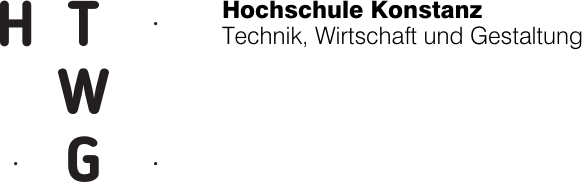
\includegraphics[width=10cm]{htwg-logo.png}
\end{flushleft}

\vspace{2.5cm}

\begin{center}
	\huge{
		\textbf{\thema} \\[5cm]
	}
	\Large{
		\textbf{\autor}} \\[6.5cm]
	\large{
		\textbf{Konstanz, \abgabedatum} \\[2.3cm]
	}
	
	\Huge{
		\textbf{{\sf MASTERARBEIT}}
	}
\end{center}

\end{titlepage}

\thispagestyle{empty}
{
\setlength{\parskip}{0.5cm}
        \begin{center}
        \textbf{\huge MASTERARBEIT}

        \textbf{zur Erlangung des akademischen Grades}

        \textbf{\Large Master of Science (M. Sc.)}

        \textbf{an der}

        \textsf{\huge Hochschule Konstanz}\\
        {\small Technik, Wirtschaft und Gestaltung}

        \textsf{\Large Fakultät Informatik} \\
        Studiengang \studiengang
        \end{center}
}
\begin{center}

\vspace*{2cm}

\begin{tabular}{p{3cm}p{10cm}}
Thema: & \textbf{\large \thema} \\[15ex]
Masterkandidat: & \autor, \autorStrasse, \autorPLZ\ \autorOrt \\[15ex]
1. Prüfer: & \prueferA \\
2. Prüfer: & \prueferB \\[25ex]
Ausgabedatum: & \ausgabedatum \\
Abgabedatum: & \abgabedatum \\
\end{tabular}
\end{center}


\hypersetup{pageanchor=true}
\pagenumbering{Roman} 
\setcounter{page}{1}


\chapter*{
  \begin{center}
  {\Large{Zusammenfassung (Abstract)}}
  \addcontentsline{toc}{chapter}{Abstract}
  \end{center}
}

\bigskip

\begin{center}
	\begin{tabular}{p{2.8cm}p{10cm}}
		Thema: & \thema \\
		 & \\
		Masterkandidat: & \autor \\
		 & \\
		Firma: & \firma \\
		 & \\
		Betreuer: & \prueferA  \\[.5ex]
		 &  \prueferB \\
		 & \\
		Abgabedatum: & \abgabedatum \\
		 & \\
		Schlagworte: & \schlagworte \\
		 & \\
	\end{tabular}
\end{center}

\bigskip

\noindent
\zusammenfassung

%
% TABLE OF CONTENTS
%
\renewcommand{\contentsname}{Inhaltsverzeichnis}
\tableofcontents
\thispagestyle{plain}
\newpage

\chapter*{Abkürzungsverzeichnis}
\label{chap:ACRONYM}
\addcontentsline{toc}{chapter}{Abkürzungsverzeichnis}

\begin{acronym}[Bash]
  \acro{lxc}[LXC]{Linux Container}
  \acro{vm}[VM]{Virtual Machine}

\end{acronym}

\newpage

\label{chap:FIGURES}
\renewcommand\listfigurename{Abbildungsverzeichnis}
\listoffigures
\newpage


\label{chap:LIST_OF_LISTINGS}
\renewcommand\lstlistlistingname{Quelltextverzeichnis}
\lstlistoflistings
\newpage



%Content
\pagenumbering{arabic} 
\setcounter{page}{1}
\setlength{\parindent}{0em}
\setlength{\parskip}{1em}
\renewcommand{\baselinestretch}{1}
\renewcommand\chaptername{Kapitel}
\renewcommand{\figurename}{Abbildung}
\renewcommand{\lstlistingname}{Programmcode}
\chapter{Einleitung}
\label{sec:INTRO}

\section{Problemstellung}
\label{sec:INTRO_PROBLEM}

\section{Wissenschaftliche Fragestellung}
\label{sec:INTRO_SCIENTIFIC_QUESTION}

\section{Aufbau}
\label{sec:INTRO_STRUCTURE}


\chapter{Grundlagen}
\label{sec:FUNDAMENTALS}

In diesem Kapitel werden die Grundlagen für diese Arbeit vorgestellt. Zu diesen Grundlagen gehört zuerst einmal die Einordnung des Begriffs Softwarearchitektur. Des Weiteren wird noch auf die Technologie der Containervirtualisierung eingegangen.

\section{Softwarearchitektur}
\label{sec:FUNDAMENTALS_ARCHITECTURE}

Der Vorgang zur Erstellung der Architektur einer Software, auch Softwarearchitektur genannt, wird definiert als Prozess des Entwerfens, Definierens, Ausdrucks, Dokumentierens, Kommunizierens, Zertifizierens der korrekten Implementierung, Wartung und Verbesserung einer Architektur während des gesamten Lebenszyklus eines Systems \cite{ISO_IEC_42010}. Dabei besteht die Softwarearchitektur aus den grundlegenden Konzepten oder Eigenschaften eines Systems in seiner Umgebung, verkörpert in seinen Elementen, Beziehungen und in den Prinzipien seines Designs und seiner Entwicklung. Weiterhin ist die Umgebung eines Systems ein Kontext, der die Einstellung und die Umstände aller Einflüsse auf ein System bestimmt. Die Umgebung eines Systems umfasst entwicklungspolitische, technologische, betriebswirtschaftliche, betriebliche, organisatorische, politische, ökonomische, rechtliche, regulatorische, ökologische und soziale Einflüsse.

Die Softwarearchitektur gehört zum Themenfeld des Softwareentwurfs. Jedoch ist nicht alles in einem Softwareentwurf auch gleichzeitig ein Teil der Softwarearchitektur. Vereinfacht dargestellt, bietet die Softwarearchitektur eine strukturelle Übersicht einer Software und beinhaltet Lösungen für strukturelle Entscheidungen, die sich im nachhinein nur mit sehr viel Aufwand ändern lassen. Die Softwarearchitektur ist somit ein grober Entwurf und lässt sich von einem Detailentwurf einer Software abgrenzen. Formal lässt sich eine genaue Trennung der Entwürfe jedoch nur schwer definieren.

\section{Modellgetriebene Softwareentwicklung}
\label{sec:FUNDAMENTALS_MDSD}

Die Anwendung von Modellen in der Softwareentwicklung hat eine lange Tradition und ist seit der Entwicklung der \ac{uml} noch populärer geworden, die Beziehung zwischen Modell und Softwareimplementierung ist nur bewusst, aber nicht formal \cite[S. 3-4]{mdsd}. Sie hat zwei gravierende Nachteile: Zum einen sind Softwaresysteme nicht statisch und unterliegen insbesondere in den ersten Phasen ihres Lebenszyklus erheblichen Veränderungen. Die Dokumentation muss daher akribisch angepasst werden, was eine komplexe Aufgabe sein kann - je nachdem, wie detailliert sie ist - oder sie wird inkonsistent. Andererseits fördern solche Modelle nur indirekt den Fortschritt, da es die Interpretation des Software-Entwicklers ist, die schließlich zu implementierten Programmcode führt. Das sind die Gründe, warum - verständlicherweise - viele Programmierer Modelle als Overhead und bestenfalls als Zwischenergebnisse betrachten. \ac{mdsd} hat einen ganz anderen Ansatz: Modelle stellen keine Dokumentation dar, sondern sind dem Code gleichgestellt, da ihre Implementierung automatisiert ist. \ac{mdsd} zielt daher darauf ab, domänenspezifische Abstraktionen zu finden und durch formale Modellierung zugänglich zu machen. Dieses Verfahren schafft ein großes Potenzial für die Automatisierung der Softwareproduktion, was wiederum zu einer Steigerung der Produktivität führt. Darüber hinaus steigt sowohl die Qualität als auch die Wartbarkeit von Softwaresystemen. Modelle können auch von Fachleuten verstanden werden. Um das domänenspezifische Modellkonzept erfolgreich anwenden zu können, müssen drei Voraussetzungen erfüllt sein: Domänenspezifische Sprachen sind erforderlich, um die eigentliche Formulierung von Modellen zu ermöglichen, Sprachen, die die notwendigen \ac{m2t} Transformationen ausdrücken können, und Compiler, Generatoren oder Transformatoren, die die Transformationen ausführen können, um auf verfügbaren Plattformen ausführbaren Code zu erzeugen.

Eine \ac{dsl} dient dazu, die wesentlichen Aspekte einer Domain - aber nicht alle denkbaren Inhalte - formal ausformulierbar und modellierbar zu machen \cite[S. 58]{mdsd}. Dazu besitzt es ein Metamodell einschließlich seiner statischen Semantik und eine entsprechende konkrete Syntax. Das allein reicht nicht aus: Die dynamische Semantik, die notwendig ist, um den Konstrukten des Metamodells einen Sinn zu geben, fehlt noch. Die Semantik eines \ac{dsl} ist in mehrfacher Hinsicht relevant: Einerseits muss der Modellierer die Bedeutung der ihm zur Verfügung stehenden Sprachelemente kennen, um sinnvolle Modelle erstellen zu können, andererseits müssen automatische Transformationen der Modelle genau diese Semantik ausführen. \acp{dsl} können in ihrer Leistung und Komplexität variieren. Einfache textuelle Konfigurationsmöglichkeiten mit Gültigkeitstests können eine \ac{dsl} bilden, während am anderen Ende des Spektrums grafische Sprachen mit entsprechenden sprachspezifischen Editoren sein können.

\section{Webapplikation}
\label{sec:FUNDAMENTALS_WEB}

Webapplikationen laufen nicht wie eine klassische Desktopanwendung lokal auf dem eigenen PC, sondern wird auf einem Server ausgeführt und können über das Internet in einem Web Browser zugegriffen werden \cite{web_application}. Die Datenverarbeitung und -persistierung findet auf dem Server statt und die Darstellung findet wiederum im Webbrowser als Client statt. Dabei werden Daten und der Programmcode über \ac{http} übertragen. Eine Webapplikation entspricht somit einer Client-Server Architektur.

In \ac{ria} reagiert die Webseite dynamisch auf Benutzereingaben \cite{rich_internet_application}. Dies wird entweder durch proprietäre Lösung auf Basis von z.B. \textit{Flash} oder \textit{Microsoft Silverlight} oder durch den starken Einsatz von JavaScript wie z.B. mit der Bibliotheken \textit{jQuery} ermöglicht. Inzwischen kommen die proprietären Lösungen immer seltener zum Einsatz und werden nach und nach eingestellt, da \ac{html} immer mehr dieselben Funktionen von sich aus anbietet \cite{flash_end_of_life}.

\ac{spa} ist einer spezielle Art von Webapplikationen, die noch stärker einer Desktopanwendung ähnelt, da nicht mehr wie sonst eine Webseite aus untereinander referenzierten Dokumenten besteht, sondern nur noch aus einem einzigen Dokument \cite[S.~497]{javascript_definitive_guide}. Bei einer Benutzerinteraktion werden die Inhalte entsprechend dynamisch im Hintergrund nachgeladen. Dieser Ansatz ermöglicht die Entwicklung von Fat-Clients durch eine immer stärker werdende Verschiebung von Logik aus dem Server zum Client. Dies führt entsprechend zu Entlastung des Servers und gleichzeitig größeren Belastung des Web Browsers auf Seiten des Clients.

\section{Containervirtualisierung}
\label{sec:FUNDAMENTALS_CONTAINER}

In der Informatik bezeichnet der Begriff Virtualisierung ein Framework zur Trennung der Ressourcen eines Computers in mehrere Ausführungsumgebungen \cite{virtualization}. Dies kann durch Konzepte oder Technologien wie Hard- oder Software-Partitionierung, Time-Sharing, teilweise oder gänzliche Maschinensimulation oder auch -emulation realisiert werden. Dabei existieren verschiedene Arten der Virtualisierung. Bei der Hardwarevirtualisierung oder Emulation geht es um den Computers als gesamte Hardware Plattform \cite{wiki:hardware_virtual}. Dadurch ist es möglich parallel neben einem fest installiertem Betriebssystem, auch Hostsystem genannt, auf einem Computer weitere simulierte Computerumgebungen mit einem Betriebssystem als Gastsystem auszuführen. Diese werden allgemein auch als \ac{vm} bezeichnet. Dabei besteht keine Einschränkung hinsichtlich des genutzten Betriebssystems als Gastsystem. Somit ist es möglich z.B. auf einem Hostsystem mit Windows ein Gastsystem mit einem Linux basiertem Betriebssystem zu betreiben. Der umgekehrte Fall ist entsprechend auch möglich. Des Weiteren sind aufgrund der Abstraktionsschicht durch die Virtualisierung die einzelnen \acp{vm} vom Hostsystem und anderen Gastsystemen isoliert und ein Zugriff auf diese wird unterbunden. Die vollständige Isolierung konnte jedoch selbst in der jüngsten Vergangenheit nicht immer zu 100\% sichergestellt werden \cite{CVE-2017-4934}.

Eine weitere Art der Virtualisierung wird als Software- oder auch Containervirtualisierung bezeichnet \cite{software_container}. Historisch hat sich die Containervirtualisierung aus der Unix-System Operation \textit{chroot} entwickelt. Die \textit{chroot} ermöglicht die Zugriffe eines Prozesses auf ein Unterverzeichnis zu limitieren. Aus den Konzepten der \textit{chroot} Operation haben sich die heutigen \ac{lxc} entwickelt. \ac{lxc} bauen auf Standardfunktionalitäten des Linux Kernels auf und isolieren anhand von Kernel Namespaces und \textit{cgroups} die Ausführung eines Programms. Kernel Namespaces isolieren dabei mit eigenen Prozess-IDs, Dateisystem, Netzwerk und Benutzer-IDs ein Programm vom Hostsystem. Wiederum limitieren und priorisieren \textit{cgroups} die Ressourcen eines Computers wie z.B. CPU, Arbeitsspeicher oder Netzwerk. Anders als bei einer \ac{vm} wird nicht ein ganzes Betriebssystem in einer virtualisierten Umgebung ausgeführt, sondern, wie in Abbildung~\ref{fig:DOCKER_VS_VM} auf Seite~\pageref{fig:DOCKER_VS_VM} zusehen, nur einzelne Programme. Dabei kann ein Programm aus einem Hauptprozess und mehreren Subprozessen bestehen. Die virtuelle Umgebung eines einzelnen Programms wird als Container bezeichnet. Container haben in vielen Szenarien signifikante Geschwindigkeitsvorteile gegenüber \acp{vm} \cite{performance_container}. Neben den Ressourcen eines Computers nutzen alle Container denselben Betriebssystem Kernel. Jedoch können verschiedene Linux Distributionen unabhängig vom Hostsystem innerhalb der Container zur Verfügung gestellt werden. Somit findet die Virtualisierung der Container auf der Ebene des Betriebssystems statt und ist im Fall von \ac{lxc} von bestimmten Funktionalitäten des Linux Kernels abhängig. Dank \ac{lxc} ist die Containervirtualisierung auf allen Linux basierten Distributionen möglich, aber es ist auch genau auf diese limitiert und die Portabilität auf andere Kernel bedingt die Unterstützung einer ähnlichen Funktionalität zur Virtualisierung auf Ebene des Betriebssystems.

\begin{figure}
    \centering
    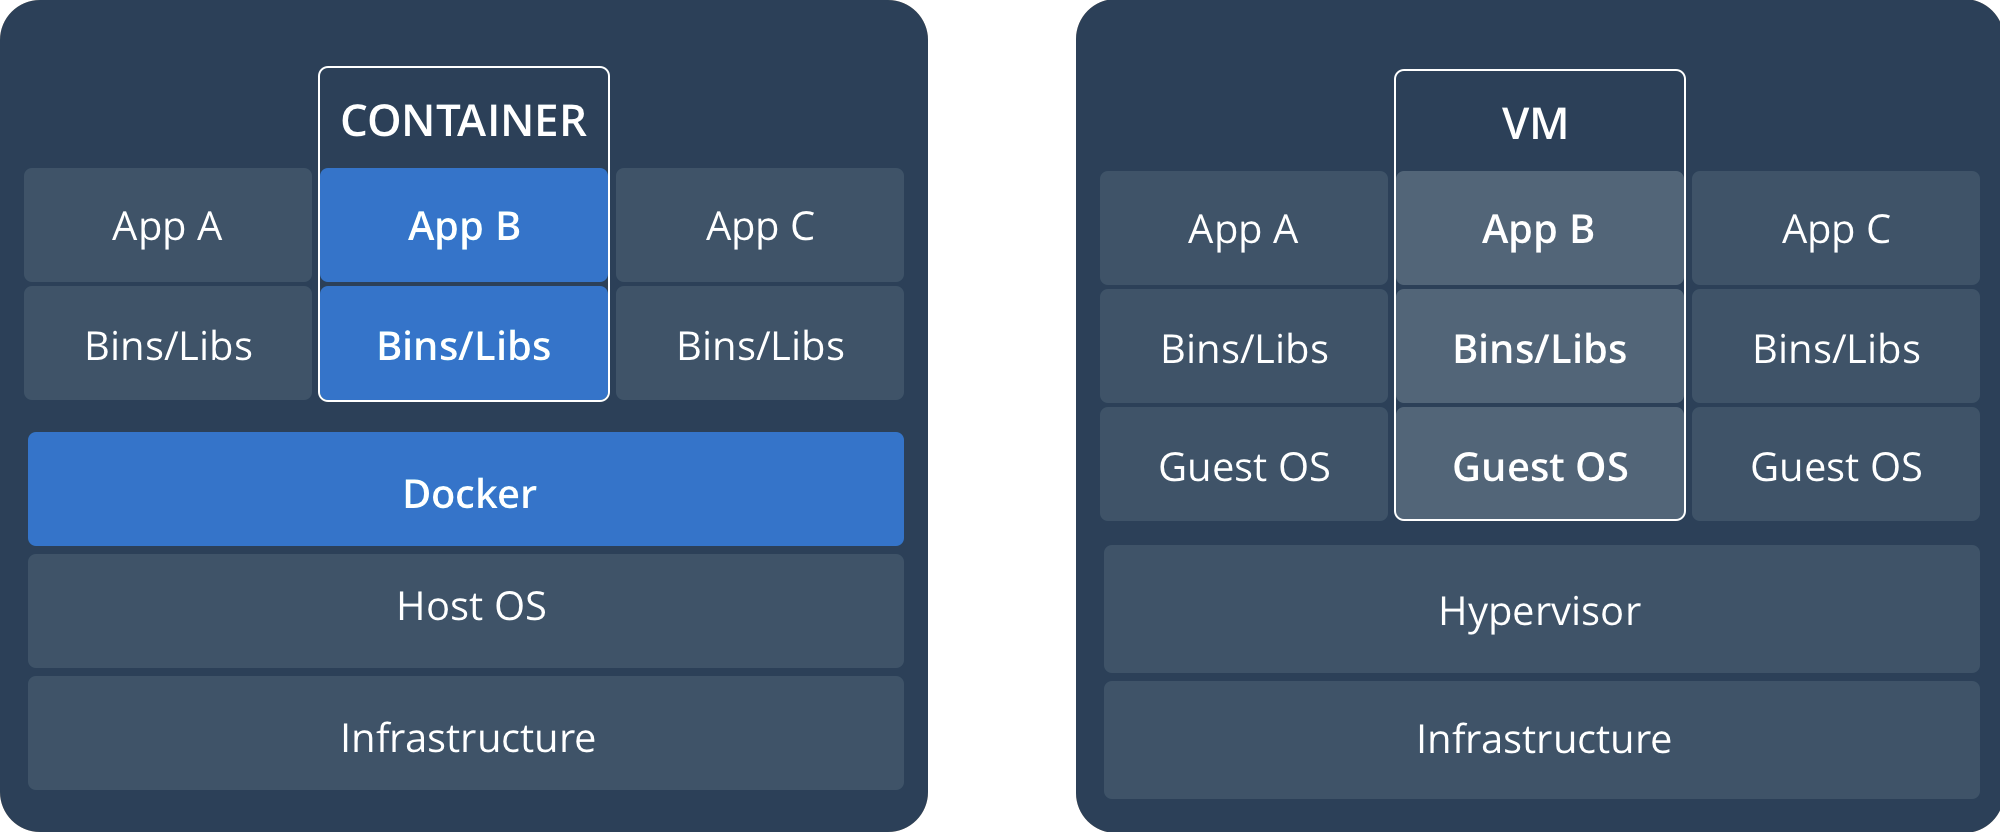
\includegraphics[width=4in]{figures/docker-vs-vm.png}
    \caption[Docker VS VM]
    {Docker VS VM \cite{what_container}}
    \label{fig:DOCKER_VS_VM}
\end{figure}

Die Open Source Plattform \textit{Docker} ist neben vielen anderen Lösungen einer der bekanntesten Vertreter der Containervirtualisierung und ist Gründer der \textit{Open Container Initiative} \cite{about_docker}. Erstmals wurde \textit{Docker} von seinem Erfinder Solomon Hykes im Jahr 2013 der Öffentlichkeit vorgestellt und hat inzwischen die Art und Weise, wie Anwendungen besonders bei Firmen mit vielen Hosts betrieben werden, revolutioniert \cite{docker_adoption}. Durch einen modularen Aufbau und einer Kooperation mit Microsoft unterstützt \textit{Docker} neben einer Variante mit einer Linux \ac{vm} inzwischen eine native Containervirtualisierung auf Windows \cite{docker_for_windows}. Über den kostenlosen \textit{Docker Compose} Client lassen sich mehrere unterschiedliche Container zu einem Bundle zusammenfassen \cite{docker_compose} und ermöglichen somit komplexe Anwendungen mit verschiedenen Diensten, die jeweils ihren eigenen Ausführungsumgebungen haben. Die verschiedenen Dienste können dabei über das Netzwerk isoliert vom Hostsystem miteinander kommunizieren. Dabei muss diese Kommunikation zwischen den Containern so wie die externe Kommunikation jeweils einzeln freigegeben werden und verfolgt somit das Prinzip Secure-by-Default. \textit{Docker} ist jedoch nicht bei einer reinen Containervirtualisierung geblieben. Mit der in den \textit{Docker} Client integrierten Erweiterung \textit{Docker Swarm} können mehrere \textit{Docker} Hosts zu einem einzigen virtuellen Host vereint werden und stellt somit ein Cluster an \textit{Docker} Hosts zur Verfügung \cite{docker_swarm}. Dabei wird per Default die Kommunikation zwischen den \textit{Docker} Hosts mit TLS verschlüsselt. Für einen \textit{Docker} Client ist es dabei unerheblich, ob nun \textit{Docker} auf demselben Host oder in einem Cluster läuft. Die API bleibt in beiden Szenarien dieselbe und führt zu einem leichten Einstieg mit \textit{Docker Swarm}.

\section{Alternative Ansätze}

Der Bereich der graphischen Modellierung ist bei weitem kein neues Themengebiet und hat schon eine über mehrere Jahrzehnte lange Geschichte \cite{paper_metaedit}. Die \textit{Eclipse Foundation} bietet z.B. mit dem \ac{gmf} die Infrastruktur zur Entwicklung von graphischen Editoren auf Basis des \textit{Eclipse Modeling Frameworks} und des \textit{Graphical Editing Frameworks} \cite{eclipse_gmf}. Das \ac{gmf} dient als Grundlage für eine ganze Reihe von Lösungen im Rahmen der graphischen Modellierung wie z.B. \textit{Sirius} oder auch \textit{Graphiti} \cite{sirius,graphiti}. Eine von \textit{Eclipse Foundation} unabhängige Lösung bietet z.B. das Produkt \textit{MetaEdit+} \cite{metaedit}. Dabei unterstützt \textit{MetaEdit+} zum einen die Erstellung einer eigenen graphischen \ac{dsl} mit entsprechenden Generatoren und zum anderen einen Editor mit dem ein Benutzer auf Basis der eigenen \ac{dsl} Modelle erstellen kann. 

Alle diese Lösungen haben eine Gemeinsamkeit. Egal, ob basierend auf dem \ac{gmf} oder nicht, alle laufen als Anwendung innerhalb eines Desktops. Webbasierte Lösungen im Bereich der graphischen Modellierungsframeworks sind bis zum jetzigen Zeitpunkt noch keine veröffentlich worden. Im Bereich der webbasierten graphischen Editoren mit einer festen \ac{dsl} existieren aber Projekte wie z.B. \textit{Node-RED} von IBM zur Flow-basierten Programmierung für Geräten des Internet of Things \cite{node_red}.

Ein weiteres Thema bei webbasierten graphischen Modellierungsframeworks ist die Ausführung von Benutzer erstellten Programmen auf einem Server im Rahmen der Generatoren. Speziell für Modellierungsframeworks wurde in diesem Bereich noch nichts veröffentlicht. Außerhalb von Modellierungsframework existieren jedoch Projekte die eine große Menge von Benutzer erstellten Programmen regelmäßig ausführen und diese in einer Art und Weise isoliert haben. Ohne dabei Ihre Infrastruktur zu gefährden. Eines dieser Projekte ist z.B. \textit{Travis CI} eine Cloud basierte Lösung für automatisierte Builds von Open Source Projekten \cite{tracis_ci}.


\chapter{Ausgangsarchitektur}
\label{ch:INITIAL}

\begin{figure}
    \centering
    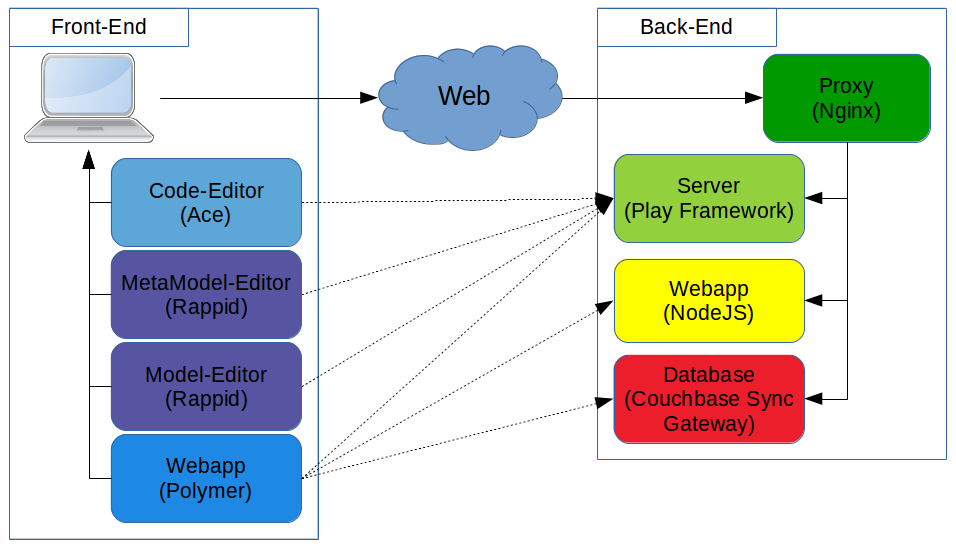
\includegraphics[width=5in]{figures/overview-before.png}
    \caption{Ausgangszustand - Übersicht}
    \label{fig:ZETA_OVERVIEW_OLD}
\end{figure}

Dieses Kapitel beschäftigt sich mit der Beschreibung des Ausgangzustands von \textit{Zeta}. Dabei wird im speziellen auf die Architektur von \textit{Zeta} und ihre Besonderheiten eingegangen. Als Ausgangszustand von \textit{Zeta} wird der Stand aus dem Git-Tag 'AktorSystem-generatorScaling' vom 11.03.2017 \cite{zeta_tag_old} verwendet.

\textit{Zeta} ist eine Webapplikation und besteht aus diesem Grund primär aus einer Client-Server Architektur. Dabei ist der Browser auf dem Computer eines Benutzers in diesem Fall der Client und ein Webserver oder Proxy entsprechend der Server. Dabei wird sämtlicher Code einer Webapplikation der im Client interpretiert und ausgeführt wird im weiteren Verlauf als Front-End und sämtlicher Code der serverseitig ausgeführt wird als Back-End bezeichnet. Eine Übersicht der Client-Server Architektur von \textit{Zeta} wird in Abbildung~\ref{fig:ZETA_OVERVIEW_OLD} auf Seite~\pageref{fig:ZETA_OVERVIEW_OLD} dargestellt. Das Front-End von \textit{Zeta} kommuniziert zentral über einen Reverse Proxy mit dem Back-End. Dabei ist das Front-End in mehrere Unteranwendungen und das Back-End in mehrere Dienste zur eigentlichen Verarbeitung der Anfragen aufgeteilt.

\section{Front-End}
\label{sec:INITIAL_FRONTEND}

Das Front-End umfasst zum einen Teil primär statische Seiten für eine Benutzer-Verwaltung mit Funktionen wie Registrieren, Anmelden und Abmelden. Des Weiteren können neue Projekte angelegt werden. In wenigen Fällen wie im  Beispiel der Projektübersicht oder der Registrierung wird per JavaScript dynamisch auf die Interaktion eines Benutzers reagiert. Die weiteren Teile des Front-Ends umfassen angefangen mit \ac{ria} bis zu \ac{spa} Anwendungen und werden im weiteren Verlauf im Detail betrachtet. Innerhalb eines Projekts wird zuerst ein Modell beschrieben. Dabei wird ein \textit{Code-Editor} zur Definition einiger Teile des Modells per textueller \acp{dsl} benutzt. Darauf folgt der graphische Editor für den \textit{MetaModel-Editor} und den \textit{Model-Editor}. Mit dem \textit{MetaModel-Editor} kann die zugrundeliegende Datenstruktur für die spätere Modell Instanz definiert werden. Aus diesen Informationen kann nun über das Back-End ein \textit{Model-Editor} generiert werden. Dieser \textit{Model-Editor} kommt beim nächsten Schritt zum Anlegen und Bearbeiten von Modell Instanzen zum Einsatz. Als nächstes wird noch die \textit{Webapp} zur Verwaltung von Generatoren benötigt. Dabei werden innerhalb der \textit{Webapp} Transformationsregeln zur \ac{m2t} Transformation angelegt. Aus den Daten der Modell Instanz und den Transformationsregeln kann nun im Back-End über Generatoren schlussendlich jegliche textuelle Form wie z.B. Programmcode in einer beliebigen Programmiersprache erzeugt werden. Im weiteren Verlauf dieses Abschnitts wird noch mal genauer auf die technischen Details des \textit{Code-Editors}, des graphischen Editors für den \textit{MetaModel-} und \textit{Model-Editor} und der \textit{Webapp} eingegangen.

\subsection{Code-Editor}

Wie zuvor erwähnt werden textuelle \acp{dsl} in Teilen zur Beschreibung des Modells genutzt und zu diesem Zweck wird ein \textit{Code-Editor} benötigt. Der \textit{Code-Editor} von \textit{Zeta} ist eine \ac{ria} Anwendung und baut auf den Open Source und selbst ernannten High Performance Code Editor für das Web namens \ac{ace} auf \cite{zeta_ace_html} \cite{zeta_ace_scala}. \ac{ace} ist der primäre Editor der webbasierten \textit{Cloud9 IDE}, welche inzwischen von Amazon unter dem Namen \textit{AWS Cloud9} vertrieben wird \cite{ace_about} \cite{ace_aws}. Die erste Version von \ac{ace} wurde 2010 veröffentlicht und wird bis heute unter anderem von Mozilla gewartet. Die Funktionen von \ac{ace} umfassen unter anderem Syntax-Highlighting mit verschiedenen Themes, automatisches Einrücken, flexible anpassbare Tastaturkürzel, eine Suche, Aus- und Einblenden einzelner Blöcke eines Programmcodes, einen \textit{Live Syntax Checker} und eine einfache Autovervollständigung.

Initial werden die Ressourcen des \textit{Code-Editors} wie \ac{html}-, \ac{css}- und JavaScript-Dateien vom \textit{Play Server} über den \textit{Proxy} Dienst an den Browser eines Benutzers ausgeliefert. Zur Laufzeit  nutzt \textit{Zeta} zur Beschreibung der Grammatik für die einzelnen textuellen \ac{dsl} die Open Source Bibliothek \textit{Ace-Grammar} \cite{ace_grammar}. Dabei wird aus einem \ac{json} Schema ein Syntax-Highlighting Parser für \ac{ace} erzeugt. Zusätzlich verbindet sich der \textit{Code-Editor} über einen Websocket mit dem \textit{Play Server}. Über diesen Websocket wird bei jeder Änderung der aktuelle Inhalt des \textit{Code-Editors} vom Browser an das Back-End übermittelt. Des Weiteren wird aber auch der \textit{Code-Editor} über den Websocket vom Back-End über den initialen und über Änderungen am Inhalt informiert, damit \ac{ace} entsprechend eine neue Sitzung mit dem aktuellen Inhalt und dem Syntax Highlighting Parser erstellt. Mit diesem Mechanismus ist es möglich, kollaborativ mit mehreren Benutzern an den Definitionen einer textuellen \ac{dsl} zu arbeiten, da der Stand zwischen den in mehreren Web Browser geöffeneten \textit{Code-Editoren} synchronisiert wird. Abschließend wird auch bei jeder Änderung des Inhalts im \textit{Code-Editor} noch der aktuelle Stand über einen Webservice des \textit{Play Servers} zusätzlich im Back-End persistiert.

\subsection{Graphischer Editor}

Der \textit{MetaModel-} und \textit{Model-Editor} in \textit{Zeta} ist eine \ac{ria} Anwendung und besteht primär aus einem graphischer Editor. \textit{Zeta} setzt hierbei auf das proprietäre \textit{Rappid Diagramm Framework} oder kurz \textit{Rappid} genannt. Der \textit{Rappid} wird von der Firma \textit{client IO} entwickelt und basiert auf der Open Source Diagramm Bibliothek \textit{JointJS} derselbigen Firma. Während \textit{JointJS} grundlegende Funktionen zur Erstellung von \acp{svg} bietet, erweitert \textit{Rappid} dieses Grundgerüst um einen vollwertigen webbasierten graphischen Editor. Hierbei kann \textit{Rappid} im Browser aus einer Palette einzelner Diagrammelemente per Drag \& Drop neue Elemente auf einer Arbeitsfläche erstellen. \textit{Rappid} unterstützt weiterhin Funktionen wie ein Backroll oder das Wiederholen von Änderungen, Realtime Kollaboration, Export als raster- oder vector-basierter Grafik und einem Inspektor zur erweiterten Bearbeitung der Inhalte eines Diagrammelements.

Der \textit{MetaModel-Editor} in \textit{Zeta} wird zur Definition eines Meta Modells eingesetzt. Dabei werden die Ressourcen für den \textit{MetaModel-Editor} vom \textit{Play Server} über den \textit{Proxy} Dienst an den Browser des Benutzers übermittelt. Der Stand des Editors wird initial beim Laden des Editors per Browser über das \ac{html} Dokument als \ac{json} in einer globalen JavaScript Variable mitgesendet und muss nicht zusätzlich über einen Webservice geladen werden. Zur Laufzeit wird \textit{Rappid} mit den zuvor definierten Diagrammelementen mit entsprechenden Inspektoren und einigen eigens für \textit{Zeta} entwickelten Erweiterungen initialisiert. Eine dieser Erweiterungen z.B. synchronisiert den aktuellen Stand des \textit{MetaModel-Editors} über mehrere im Browser geöffnete Instanzen und ermöglicht somit kollaboratives Arbeiten mehrerer Benutzer an ein und demselben Meta Modell. Eine andere Erweiterung erzeugt beim Speichern aus dem aktuellen Stand die Datenstruktur des Meta Modells und sendet diese zusammen mit weiteren Information des \textit{UI-State} wie z.B. Position, Hintergrundfarbe und etc. einzelner Diagrammelemente über einen Webservice \ac{api} an den \textit{Play Server}.

Der \textit{Model-Editor} wird dazu genutzt, um die Inhalte einer Modell Instanz zu definieren. Auch hier werden die Ressourcen des Editors über den \textit{Play Server} ausgeliefert und auch der initiale Stand des Editors wird über eine globale JavaScript Variable im \ac{html} Dokument mitgeliefert. Während im \textit{MetaModel-Editor} nur zwei Diagrammelemente benötigt werden, muss der \textit{Model-Editor} mit Diagrammelementen auf Basis der Definitionen aus den \textit{Code-Editoren} arbeiten und muss die Inhalte aus den Inspektoren auf die Datenstruktur des Meta Modells mappen. Zu diesem Zweck wird über den \textit{Generate-Button} in der Projektübersicht die Erzeugung von JavaScript Dateien für den \textit{Model-Editor} angestoßen. Anhand der Definition aus dem \textit{Code-Editor} und dem \textit{MetaModel-Editor} werden nun innerhalb des \textit{Play Servers} einzelne JavaScript Dateien zur späteren Konfiguration von \textit{Rappid} im Browser erzeugt. Bei jeder Änderung über den \textit{Code-Editor} oder \textit{MetaModel-Editor} müssen diese JavaScript Dateien erneut erzeugt werden. Auch für den \textit{Model-Editor} wurden eigens für \textit{Rappid} einige Erweiterungen programmiert. Zum Speichern werden wie auch im \textit{MetaModel-Editor} mit einem Exporter aus dem aktuellen Stand des Editors die Daten in ein bestimmtes Schema \ac{json} Schema überführt und zusammen mit dem \textit{UI-State} per Webservice \ac{api} an den \textit{Play Server} zur Persistierung übermittelt. Zusätzlich ist der \textit{Model-Editor} noch an einen Websocket des \textit{Play Servers} angebunden. Dabei wird beim Speichern das Back-End per Websocket über dieses Ereignis informiert und parallel wird der Browser bei Änderungen über die aktuelle Liste an sogenanntem und nicht näher beschriebenem \textit{BondedTask} informiert. Die Liste an \textit{BondedTask} wird im \textit{Model-Editor} dargestellt und per Klick auf einen Eintrag wird das Back-End per Websocket über das Ausführen eines \textit{Bonded-Task} beauftragt. Entsprechend informiert das Back-End den Browser per Websocket über den Start und Abschluss eines \textit{Bonded-Tasks}. Diese \textit{Bonded-Tasks} können nicht im \textit{Model-Editor} erstellt werden, sondern werden über die \textit{Webapp} erzeugt.

\subsection{Webapp}

Die \textit{Webapp} ist eine \ac{spa} mit entsprechend clientseitigem Routing und wird parallel neben dem \textit{Play Server} über einen \textit{Node.js} Server ausgeliefert. Die \textit{Webapp} basiert auf der \textit{Polymer} Bibliothek für Web Components. \textit{Polymer} wird von Google entwickelt und wurde unter anderem beim Redesign von \textit{Youtube} eingesetzt. Die \textit{Webapp} von \textit{Zeta} bietet zum einen eine Oberfläche zur Erstellung bzw. zum Anpassen eines Generators mit seinen \ac{m2t} Transformationsregeln. Zum anderen können die Generatoren gestartet und gestoppt werden. Zusätzlich können die erstellten Generatoren noch über programmierbare Filter gruppiert werden. Aufbauend auf den Generatoren und den Filtern können noch verschiedene Task wie z.B. einen \textit{Bonded-Task} oder einen \textit{Timed-Task} erstellt werden.

Dabei ist die \textit{Webapp} größtenteils unabhängig von Back-End und nutzt nur einen einzigen Websocket, um mit dem \textit{Play Server} zu kommunizieren. Über den Websocket auf der \ac{url} \textit{/socket/developer} wird der Browser zum einen in regelmäßigen Abständen über laufende Generatoren informiert und zum anderen über die Ausgaben des einzelnen Generators. Die \textit{Webapp} beauftragt wiederum das Back-End über den Websocket z.B. das Starten oder Stoppen eines Generators. Zum Teil persistieren die Generatoren während ihrer Ausführung die Daten selbstständig zum \textit{Couchbase Sync Gateway}. Die restlichen Daten werden clientseitig im Browser zum \textit{Couchbase Sync Gateway} persistiert. Dabei greift die \textit{Webapp} nicht direkt, sondern entsprechend über den \textit{Proxy} Dienst auf das \textit{Sync Gateway} zu. Die notwendige Sitzung für die Authentifizierung am \textit{Sync Gateway} wurde zuvor bei der Anmeldung des Benutzers am \textit{Play Server} initiiert. Des Weiteren ist die \textit{Webapp} über ein Websocket an einen \textit{Live Change Feed} des \textit{Sync Gateways} angeschlossen. Falls nun Dokumente der Datenbank über das \textit{Sync Gateway} angepasst werden, wird die \textit{Webapp} über diese Änderung informiert und aktualisiert entsprechend die vorgehaltenen Daten.

\section{Back-End}

Das Back-End von \textit{Zeta} besteht aus einer Reihe von auf ihren Anwendungsfall spezialisierten Diensten. Jeder Dienst wird isoliert von den anderen Diensten des Betriebssystems und den einzelnen Diensten von \textit{Zeta} in einem \textit{Docker Container} ausgeführt. Dabei sind die verschiedenen \textit{Docker Container} bei \textit{Zeta} zu einem Verbund zusammengefasst. Dieser Verbund ist per \textit{Docker Compose} definiert \cite{zeta_docker_compose}. Eine Übersicht dieser Dienste mit ihren Kommunikationskanälen können in Abbildung~\ref{fig:ZETA_ARCH_OLD} auf Seite~\pageref{fig:ZETA_ARCH_OLD} eingesehen werden. Dabei wird in der Abbildung zwischen den initial gestarteten Containern von \textit{Docker Compose} und den Containern des \textit{Docker Compose} Netwerks unterschieden, da \textit{Zeta} zur Laufzeit je Generator einen Container über den \textit{Docker Daemon} startet und diesen zusätzlich dem Netzwerk der \textit{Docker Compose} Instanz beitreten lässt. Die \textit{Docker Container} der Generatoren müssen dem \textit{Docker Compose} Netzwerk von \textit{Zeta} beitreten, da das private Netzwerk der \textit{Docker Compose} Instanz nur ganz gezielt externen Zugriff zulässt und die Generatoren einen Zugriff auf den einen oder anderen Dienst von \textit{Zeta} benötigen.

\begin{figure}
    \centering
    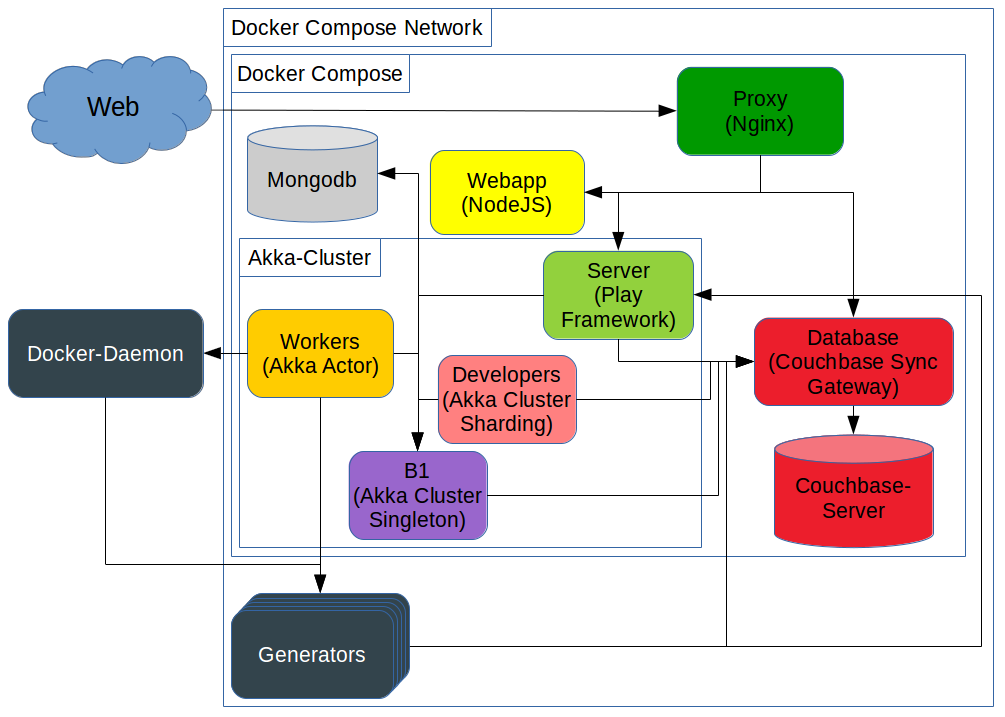
\includegraphics[width=5in]{figures/docker-compose-before.png}
    \caption{Ausgangszustand - Dienste}
    \label{fig:ZETA_ARCH_OLD}
\end{figure}

Auf der höchsten Ebene der Dienste fungiert im Back-End von \textit{Zeta} ein \textit{Nginx} Server als Reverse Proxy und ist somit die öffentliche \ac{api} für sämtliche Anfragen der Benutzer aus dem \ac{www}. Von dem Reverse Proxy aus werden die Anfragen entsprechend der genutzten \ac{url} an den \textit{Webapp} Dienst, das \textit{Couchbase Sync Gateway} oder den \textit{Play Server} verteilt. Der \textit{Webapp} Dienst ist ein auf \textit{Node.js} basierender Webserver und seine primäre Aufgabe ist es, die Ressourcen der \textit{Webapp} auszuliefern. Zusätzlich fungiert die Erweiterung \textit{Browsersync} als Proxy innerhalb des \textit{Webapp} Diensts und umfasst unter anderem Funktionen wie automatischer Pagereload bei Änderungen am Programmcode der \textit{Webapp} oder synchronisiertes Ausführen von Scroll und Klick Events über mehrere Browser Instanzen. \textit{Browsersync} wird hauptsächlich zu Testzwecken z.B. von verschiedenen Geräten auf Entwicklersystemen eingesetzt. Als zweites leitet der Reverse Proxy die Anfragen an die \ac{rest} \ac{api} oder die Websockets des \textit{Couchbase Sync Gateways} weiter. Zum einen fungiert das \textit{Sync Gateway} als Proxy zu einem Cluster aus einem oder mehreren \textit{Couchbase Servern} und zusätzlich wird z.B. über den \textit{Sync Endpoint} per Websocket ein \textit{Change Feed} zur Verfügung gestellt. Als letztes werden die Anfragen noch an den \textit{Play Server} weitergeleitet. Der \textit{Play Server} basiert auf dem in Scala geschriebenen \textit{Play Web Framework} und ist die ehemalige Kernkomponente von \textit{Zeta}. Der \textit{Play Server} umfasst eine Reihe an unterschiedlichen Funktionalitäten und ist nur ein Unterprojekt unter mehreren innerhalb eines größeren Scala Projekts. Zum einen bietet der \textit{Play Server} die webbasierte Oberfläche zur Benutzer- und Projektverwaltung, den \textit{Code-Editor}, den \textit{MetaModel-} und \textit{Model-Editor}. Zum anderen bietet er eine Reihe von Webservice \acp{api} und Websockets an. Dabei werden im Besonderen einige Anfragen der Websockets zu den Microservices zur Generatorverwaltung innerhalb des \textit{Akka Clusters} weitergereicht.

Im weiteren Verlauf dieses Abschnitts wird zuerst auf das Build System von \textit{Zeta} eingegangen. Dabei wird zum einen der Build Vorgang der eigens für \textit{Docker Compose} erzeugten \textit{Docker Images} betrachtet und zum anderen die Konfiguration von \ac{sbt} für die einzelnen Unterprojekte des Scala Projekts. Danach folgt eine genauere Betrachtung der Webservice \ac{api} und Websockets des \textit{Play Server} und der Teilkomponenten des \textit{Play Servers} wie dem \textit{SprayParser} mit seiner Notwendigkeit für die drei textuellen \acp{dsl}. Weitergehend werden die Aufgaben des \textit{Akka Clusters} mit der \ac{m2t} Transformation betrachtet. Abschließend wird die Rolle der \textit{Mongodb} und des \textit{Couchbase Servers} mit seinem \textit{Sync Gateway} im Detail beschrieben.

\subsection{Build-System}
\label{sec:INITIAL_BUILD}

\begin{figure}
    \centering
    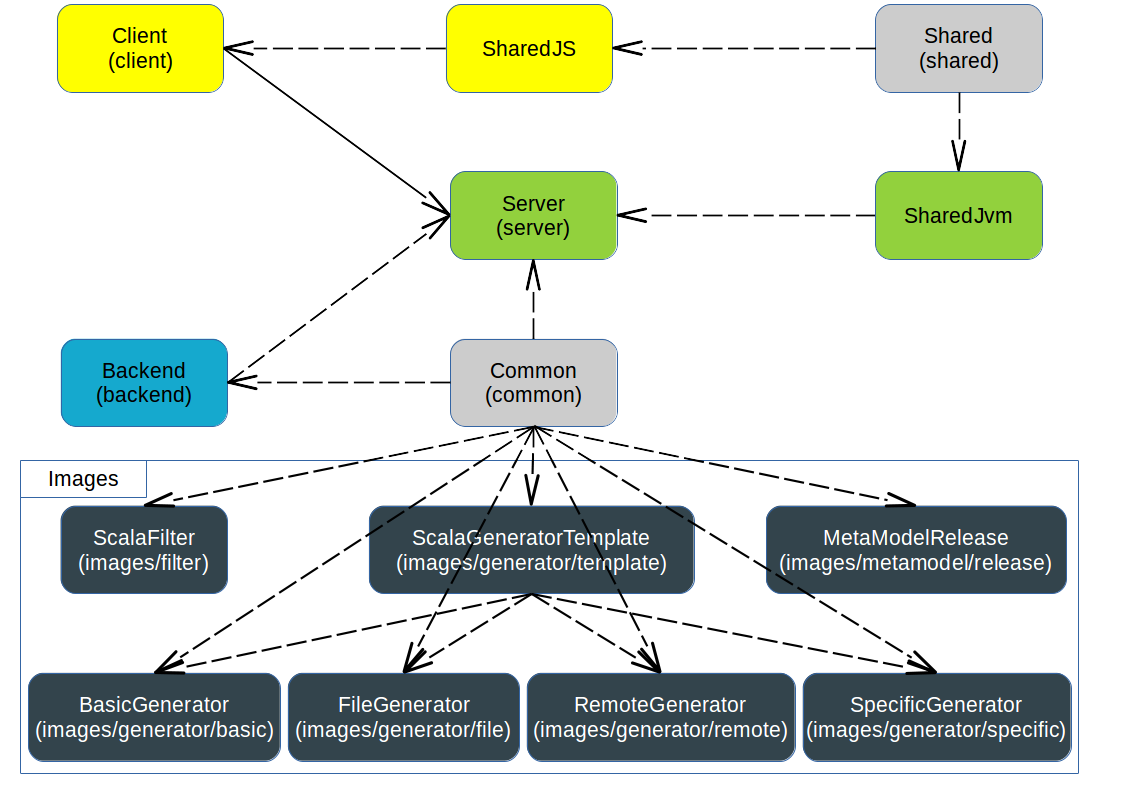
\includegraphics[width=5in]{figures/sbt-modules-before.png}
    \caption{Ausgangszustand - SBT Unterprojekte}
    \label{fig:ZETA_SBT_OLD}
\end{figure}

In diesem Unterabschnitt geht es zuerst um den Build Vorgang für die \textit{Docker Images} der einzelnen Dienste von \textit{Zeta} und darauf folgt ein tieferer Einblick in die \ac{sbt} Konfiguration des Scala Projekts. Die Laufzeitumgebung für ganz \textit{Zeta} mit den verschiedenen Diensten ist über \textit{Docker Compose} definiert \cite{zeta_docker_compose}. Für die einzelnen Dienste werden auf ihre Laufzeitumgebung optimierte \textit{Docker Images} verwendet. Dabei sind die \textit{Docker Images} nicht von Grund auf neu definiert, sondern erweitern schon bestehende öffentliche \textit{Docker Images}. Bevor die Container für die einzelnen Dienste gestartet werden können, müssen die Images in einem Build Vorgang von \textit{Docker} erzeugt werden. Dieser Vorgang wird automatisch von \textit{Docker Compose} beim Starten ausgeführt, falls die \textit{Docker Images} nicht vorhanden sind oder die genutzten Dateien für das Image sich geändert haben. Der \textit{Proxy} Dienst baut auf dem offiziellen Image für \textit{Nginx} auf und fügt zusätzlich noch eine Konfigurationsdatei zur Weiterleitung des Traffic an den entsprechenden Dienst hinzu. Der Zugriff auf diese Dienste wird beim Starten des Containers über sogenannte Links ermöglicht. Zusätzlich wird noch der Standard Port für \ac{http} des Webservers öffentlich für alle Netzwerkschnittstellen freigegeben. Beim Image für den \textit{Couchbase Server} Dienst wird auch auf dem offiziellen Image aufgebaut. Dabei wird der reguläre \textit{ENTRYPOINT} des Image mit einem eigenen ausgetauscht. Dieser neue \textit{ENTRYPOINT} erweitert den regulären \textit{ENTRYPOINT} mit der Funktionalität beim ersten Start eine Datenbank mit einem Benutzer und Passwort zu erstellen. Zur Laufzeit des \textit{Docker Containers} werden noch der Name der Datenbank, der Benutzer und das Password übergeben und einige Ports des \textit{Couchbase Servers} für den öffentlichen Zugriff freigegeben. Alle Dateien eines \textit{Docker Containers}, die zur Laufzeit erstellt worden sind, werden beim Löschen des Containers entfernt und aus diesem Grund wird der Ordner mit Daten der Datenbank per \textit{Bind Mount} persistiert. Beim \textit{Database} Dienst baut das Image auf dem offiziellen \textit{Sync Gateway} Image von Couchbase auf. Dabei wird für das Image eine eigene Konfigurationsdatei zum \textit{Couchbase Server} und ein \textit{ENTRYPOINT} hinzugefügt. Der eigene \textit{ENTRYPOINT} wartet zu Beginn auf die Erreichbarkeit des \textit{Couchbase Servers} und startet anschließend das \textit{Sync Gateway} mit dem Pfad zur eigenen Konfigurationsdatei. Beim \textit{Webapp} Dienst wird beim Image entsprechend auf dem  offiziellen \textit{Node.js} Image aufgebaut. Für das Image kommt zuerst \ac{npm} zum Auflösen der Abhängigkeiten wie den Webserver für \textit{Polymer}, die \textit{Browsersync} Erweiterung und \textit{Bower} zum Einsatz. Nachfolgend wird noch \textit{Polymer} mit seinen Abhängigkeiten per \textit{Bower} heruntergeladen. Zum Schluss wird einmal der gesamte Programmcode der \textit{Webapp} in das Image kopiert. Zur Laufzeit wird zusätzlich nochmal der gesamte Programmcode der \textit{Webapp} in den Container per \textit{Bind Mount} gemapped und die Ordner mit den heruntergeladenen Abhängigkeiten auf ein Volume gemapped. Auch für den \textit{Webapp} Dienst werden verschiede Ports des Webservers und des \textit{Browsersync} Proxys für den öffentlichen Zugriff freigegeben. Für den \textit{Mongodb} Dienst wird nur das offizielle Image benutzt und kein eigenes. Zur Laufzeit wird der Port des \textit{Mongodb} Servers freigegeben und die Daten per \textit{Bind Mount} persistiert. Für die weiteren Dienste wie dem des \textit{Play Servers} werden auch eigene Docker Images benötigt, doch diese werden nicht von \textit{Docker Compose} erzeugt, sondern müssen zuvor über ein Setupscript per \ac{sbt} wie im Programmcode~\ref{lst:ZETA_SETUP} auf Seite~\pageref{lst:ZETA_SETUP} erzeugt werden. Innerhalb dieses Setupscript wird neben den \textit{Docker Images} der \ac{sbt} Unterprojekte noch ein Image zum initialen Befüllen der Datenbank über ein \textit{Node.js} Script erzeugt. Nachdem die Datenbanken von \textit{Docker Compose} gestartet worden sind, muss einmalig ein \textit{Docker Container} mit diesem Image gestartet werden.

\bigskip
\begin{lstlisting}[caption={[Zeta Setupscript]Zeta Setupscript \cite{zeta_setupscript}},label={lst:ZETA_SETUP}]
pushd api
sbt 'project backend' 'docker:publishLocal'
sbt 'project server' 'docker:publishLocal'
sbt 'project scalaFilter' 'docker:publishLocal'
sbt 'project basicGenerator' 'docker:publishLocal'
sbt 'project fileGenerator' 'docker:publishLocal'
sbt 'project specificGenerator' 'docker:publishLocal'
sbt 'project remoteGenerator' 'docker:publishLocal'
popd

docker-compose build

pushd data
docker build -t modigen:data .
popd
\end{lstlisting}
\smallskip

Der \textit{Play Server} ist wie zuvor erwähnt nur eines von mehreren Unterprojekten innerhalb eines Scala Projekts und eine Übersicht aller Scala Unterprojekte mit ihrena Abhängigkeiten untereinander kann in Abbildung~\ref{fig:ZETA_SBT_OLD} auf Seite~\pageref{fig:ZETA_SBT_OLD} eingesehen werden. Dabei steht unterhalb jedes Unterprojekts der entsprechende Ordner innerhalb des Scala Projekts. \textit{Zeta} nutzt \ac{sbt} für den Build Vorgang des Scala Projekts. \ac{sbt} ist ein Buildtool für Java, Scala und mehr \cite{sbt}. Die Funktionalitäten von \ac{sbt} umfassen zum einen das Auflösen der zuvor definierte \ac{sbt} Version und die Abhängigkeiten der verschiedenen Scala Unterprojekte von Zeta \cite{zeta_api_built}. Zum anderen kann \ac{sbt} noch durch sogenannte Plugins erweitert werden. Eine Liste der genutzten Plugins für \textit{Zeta} kann in der Tabelle~\ref{tab:ZETA_SBT_OLD} auf Seite~\pageref{tab:ZETA_SBT_OLD} gefunden werden. Die ersten beiden \ac{sbt} Plugins namens \textit{sbt-revolver} und \textit{sbt-scalariform} sollen allgemein die Entwicklung unterstützen. Das nächste \ac{sbt} Plugin ist primär für die Einbindung des \textit{Play Frameworks} in \ac{sbt} zuständig. Neben einigen Funktionalitäten zur Vereinfachung der Entwicklung, baut es auch auf \textit{SbtWeb} auf. \textit{SbtWeb} ist für die Verwaltung und Auflösung von Assets zuständig und war ursprünglich Teil des \textit{Play Frameworks} \cite{sbtweb}. Zusätzlich erkennt \textit{SbtWeb} noch \textit{WebJars}. \textit{WebJars} enthalten den Programmcode bekannter Frontend Bibliotheken, wie z.B. \textit{jQuery} oder auch \textit{Bootstrap}, und können als reguläre Abhängigkeit per \ac{sbt} zu einem Scala Projekt hinzugefügt werden. Neben den \textit{WebJars} enthält der \textit{Play Server} von \textit{Zeta} noch Kopien einiger der genutzten JavaScript Bibliotheken wie z.B. \ac{ace} oder auch \textit{Rappid}. Mit \textit{SbtWeb} werden zur Laufzeit des \textit{Play Server} der Inhalt der \textit{WebJars} sowie die weiteren Dateien von Assets über den Webserver öffentlich zur Verfügung gestellt. Bei den sogenannten Assets handelt es sich bei \textit{SbtWeb} um Ressourcen für den Browser wie z.B. Datei mit JavaScript, \ac{css} oder auch um Bilder. Damit \textit{SbtWeb} die Existens dieser Assets erkennen kann, müssen diese in entsprechenden Ordnern vorhanden sein. Alle weiteren \ac{sbt} Plugins für \textit{Zeta} erweitern nur noch die Funktionalität von \textit{SbtWeb}, wie z.B. das \textit{sbt-cofffeescript} Plugin als CoffeeScript zu JavaScript Compiler.

\begin{table}[ht]
    \smallskip
    \centering
    \begin{tabular}{| l | l | c | l |}
    \hline
    \bf GroupID & \bf ArtifactID & \bf SbtWeb & \bf Beschreibung \\ \hline
    io.spray & sbt-revolver & & Restart bei Änderung \\ \hline
    org.scalariform & sbt-scalariform & & Programmcode Formatierung \\ \hline
    com.typesafe.play & sbt-plugin & \checkmark & Dev Featues für Play \\ \hline
    com.typesafe.sbt & sbt-coffeescript & \checkmark & CoffeeScript Compiler  \\ \hline
    com.typesafe.sbt & sbt-gzip & \checkmark & Gzipped Web Assets \\ \hline
    com.vmunier & sbt-play-scalajs & \checkmark & ScalaJS für Play Framework\\ \hline
    org.scala-js & sbt-scalajs & & ScalaJS \\ \hline
    \end{tabular}
    \caption{Ausgangszustand - SBT Plugins \cite{zeta_sbt_plugins}}
    \label{tab:ZETA_SBT_OLD}
\end{table}

Wie in der Abbildung~\ref{fig:ZETA_SBT_OLD} auf Seite~\pageref{fig:ZETA_SBT_OLD} zusehen, hängt der \textit{Play Server} von einigen anderen Unterprojekten ab. Eines davon ist das \textit{Client} Projekt. Das \textit{Client} Projekt baut auf \textit{ScalaJS} und dem \textit{sbt-play-scalajs} Plugin zur Zusammenarbeit zwischen \textit{ScalaJS} und dem \textit{Play Framework} auf. Alle \textit{ScalaJS} Projekte sind in der Abbildung~\ref{fig:ZETA_SBT_OLD} auf Seite~\pageref{fig:ZETA_SBT_OLD} mit einer grauen Hintergrundfarbe markiert. Die Aufgabe von \textit{ScalaJS} ist es, als Scala zu JavaScript Compiler zu fungieren. Innerhalb von \textit{ScalaJS} können schon bestehende JavaScript Bibliotheken wie z.B. \textit{jQuery} genutzt werden. Damit während des Build Prozesses die Referenzen zu der \acp{api} der in JavaScript geschriebenen Bibliotheken aufgelöst werden können, müssen sogenannte \textit{Facades} vorhanden sein. Die \textit{Facades} bieten einen Mechanismus um die nicht vorhandenen Typ Informationen für die JavaScript Bibliotheken innerhalb von Scala zu definieren. Für ein paar der bekannteren JavaScript Bibliotheken wie z.B. \textit{jQuery} werden Pakete mit den Typ Informationen für \textit{ScalaJS} angeboten. Dabei enthalten diese Pakete aber nicht den Programmcode der JavaScript Bibliotheken. Sondern dieser muss noch z.B. über \textit{WebJars} in das \textit{Play Framework} eingebunden werden. Eingebunden wird das \textit{Client} Projekt in den \textit{Play Server} über die \textit{Pipeline Stages} von \textit{SbtWeb} und einer Reference als \textit{ScalaJS} Projekt. Dabei kann über die \textit{Pipeline Stages} von \textit{SbtWeb} noch die Form des generierten JavaScript zwischen einer stark optimierten Variante für den Produktivbetrieb oder einer deutlich lesbareren Variante für ein Entwicklersystem entschieden werden. Inhaltlich geht es bei \textit{Client} Projekt um die Konfiguration und Initialisierung des \textit{Code-Editors} und die eigentliche Einbindung erfolgt dabei, wie in Programmcode~\ref{lst:PLAY_CODE_EDITOR} auf Seite~\pageref{lst:PLAY_CODE_EDITOR} zusehen, innerhalb eines Templates im \textit{Play Server}.

\bigskip
\begin{lstlisting}[caption={[Lade und initialisiere Client]Lade und initialisiere Client \cite{zeta_load_client}},label={lst:PLAY_CODE_EDITOR}]
@playscalajs.html.selectScript("client", "/assets")

<script type="text/javascript">
  client.Main().main("@uuid", "@dslType");
</script>
\end{lstlisting}
\smallskip

Das \textit{Client} Projekt besitzt zusätzlich noch als einziges Scala Projekt eine interne Abhängigkeit auf das \textit{SharedJS} Projekt. Dabei ist das \textit{SharedJS} Projekt ein \textit{ScalaJS} Projekt und zusätzlich kein vollwertiges \ac{sbt} Projekt im eigentlichen Sinn. Stattdessen wird das \textit{SharedJS} Projekt aus dem \textit{Shared} Projekt erzeugt. Das \textit{Shared} Projekt wiederrum ist ein sogenanntes \textit{CrossProject} und ermöglicht es, dieselbe Codebase zum einen als \textit{ScalaJS} Projekt und zum anderen als ein reguläres \ac{sbt} Projekt als Abhängigkeit einzubinden. Aus diesem Grund werden aus dem \textit{Shared} Projekt die beiden Projekte \textit{SharedJS} und \textit{SharedJvm} erzeugt. Das \textit{SharedJvm} Projekt wird wiederum vom \textit{Play Server} als Abhängigkeit eingebunden. Das \textit{Shared} Projekt besteht nur aus zwei Scala Dateien und diese beinhalten zum einen das Kommunikationsobjekte für den Websocket des \textit{Code-Editors} und den Actor für das sogenannte \textit{DataVis} Feature des \textit{Model-Editors}.

Während die oberen Projekte auf der Abbildung~\ref{fig:ZETA_SBT_OLD} auf Seite~\pageref{fig:ZETA_SBT_OLD} primäre dem \textit{Play Server} zuarbeiten, handelt es sich bei den unteren Projekten um die späteren Generatoren. Dabei benötigen diese Unterprojekte sowie das Back-End Projekt keine \ac{sbt} Plugins. Diese Generatoren werden zur Laufzeit als \textit{Docker Container} vom \textit{Akka Cluster} des Back-End Projekts gestartet und verwenden dazu die zuvor erzeugten \textit{Docker Images}. Innerhalb der Generatoren werden die zuvor über die \textit{Webapp} erstellten und in Scala geschriebenen Transformationsregeln zur \ac{m2t} Transformation ausgeführt. Dazu werden die Transformationsregeln über die \textit{Toolbox} des Scala Compilers geparst, kompiliert und schlussendlich ausgeführt.

\subsection{Webservice API}

Für das Meta Modell und dem Modell werden von \textit{Play Server} entsprechend der Operationen zum Erstellen, Ändern, Löschen oder Auflisten \ac{rest} \acp{api} bereitgestellt. Eine Liste der verschiedenen \ac{rest} Endpoints für das Meta Modell kann in der Tabelle~\ref{tab:ZETA_REST_META_MODEL_OLD} auf Seite~\pageref{tab:ZETA_REST_META_MODEL_OLD} eingesehen werden. Für das Modell sind die verschiedenen Endpoints in der Tabelle~\ref{tab:ZETA_REST_MODEL_OLD} auf Seite~\pageref{tab:ZETA_REST_MODEL_OLD} zu finden. Dabei sind in den Tabellen die innerhalb von \textit{Zeta} genutzten Endpoints grün und die ungenutzten Endpoints mit rot markiert. Die \ac{rest} \ac{api} verwendet für die Ein- und Rückgabe jeweils eigene \ac{json} Schemata. Dabei kommen aufseiten des \textit{Play Servers} Formatierer, zur Umwandlung des internem Modells zum \ac{json} Schema und wieder zurück, zum Einsatz.

\begin{table}[ht]
    \smallskip
    \centering
    \begin{tabular}{| l | l |}
    \hline
    \bf Method & \bf Route \\ \hline
    \colorbox{red}{GET},\colorbox{LimeGreen}{POST} & /metamodels \\ \hline
    \colorbox{red}{GET},\colorbox{red}{PUT},\colorbox{LimeGreen}{DELETE} & /metamodels/\emph{:id} \\ \hline
    \colorbox{LimeGreen}{GET},\colorbox{LimeGreen}{PUT} & /metamodels/\emph{:id}/definition \\ \hline
    \colorbox{LimeGreen}{GET} & /metamodels/\emph{:id}/definition/mclasses \\ \hline
    \colorbox{LimeGreen}{GET} & /metamodels/\emph{:id}/definition/mreferences \\ \hline
    \colorbox{red}{GET} & /metamodels/\emph{:id}/definition/mclasses/\emph{:name} \\ \hline
    \colorbox{red}{GET} & /metamodels/\emph{:id}/definition/mreferences/\emph{:name} \\ \hline
    \colorbox{red}{GET},\colorbox{LimeGreen}{PUT} & /metamodels/\emph{:id}/shape \\ \hline
    \colorbox{red}{GET},\colorbox{LimeGreen}{PUT} & /metamodels/\emph{:id}/style \\ \hline
    \colorbox{red}{GET},\colorbox{LimeGreen}{PUT} & /metamodels/\emph{:id}/diagram \\ \hline
    \end{tabular}
    \caption{Ausgangszustand - Rest Meta Modell Endpoints}
    \label{tab:ZETA_REST_META_MODEL_OLD}
\end{table}

Neben der \ac{rest} \ac{api} wird über einen weiteren Endpoint für jedes, über die Oberfläche angelegte, Projekt noch eine Reihe, von zuvor generierten, JavaScript Dateien zur Verfügung gestellt. Diese Dateien sind zur Konfiguration des graphischen Editors einer Modell Instanz notwendig. Die Konfiguration basiert auf den zuvor per \textit{Code-} und \textit{MetaModel-Editor} erstellten Definitionen aus dem Modell des Projekts. Zu diesem Zweck werden innerhalb des \textit{Play Server} diese Definitionen geparst und über einen internen Generator die einzelnen JavaScript Dateien erzeugt. Dabei muss die Erzeugung der JavaScript Dateien initial und bei jeder Änderung am Modell von Hand über den \textit{Generate-Button} in der Projektübersicht angestoßen werden.

\begin{table}[ht]
    \smallskip
    \centering
    \begin{tabular}{| l | l |}
    \hline
    \bf Method & \bf Route \\ \hline
    \colorbox{red}{GET},\colorbox{LimeGreen}{POST} & /models \\ \hline
    \colorbox{LimeGreen}{GET},\colorbox{red}{PUT},\colorbox{LimeGreen}{DELETE} & /models/\emph{:id} \\ \hline
    \colorbox{red}{GET},\colorbox{LimeGreen}{PUT} & /models/\emph{:id}/definition \\ \hline
    \colorbox{red}{GET} & /models/\emph{:id}/definition/nodes \\ \hline
    \colorbox{red}{GET} & /models/\emph{:id}/definition/nodes/\emph{:name} \\ \hline
    \colorbox{red}{GET} & /models/\emph{:id}/definition/edges \\ \hline
    \colorbox{red}{GET} & /models/\emph{:id}/definition/edges/\emph{:name} \\ \hline
    \end{tabular}
    \caption{table}{Ausgangszustand - Rest Modell Endpoints}
    \label{tab:ZETA_REST_MODEL_OLD}
\end{table}

\subsection{Websockets}

Um für bestimmte Anwendungsfälle für den \textit{Code-}, \textit{MetaModel-}, \textit{Meta-Editor} oder die Generator Verwaltung in der \textit{Webapp} in Echtzeit über Veränderungen informiert zu werden, bietet \textit{Zeta} über eine Reihe von Endpoints im \textit{Play Server} Websockets an. Dabei werden die Websockets im \textit{Play Server} per \textit{Akka Actoren} implementiert, um eine bidirektionale Kommunikation und eine asynchronen Workflow während der offenen Socket Verbindung zu ermöglichen. Wie in Abbildung~\ref{fig:ZETA_WS_OLD} auf Seite~\pageref{fig:ZETA_WS_OLD} dargegestellt lassen sich die Websockets grob in zwei Kategorien einteilen. Die Actoren der oberen Websockets sind Teil des Back-End Projekts und kommunizieren mit dem \textit{Akka Cluster} der Generatoren. Die Actoren der unteren Websockets sind wiederum Teil des \textit{Play Servers} und ermöglichen so z.B. eine Synchronisation desselben Stands eines über mehrere Browser geöffneten \textit{Code-Editors}. Somit lässt sich kollaboratives Arbeiten für den \textit{Code-Editor} über einen Websocket ermöglichen. Des Weiteren wird auch für den graphischen Editor des Meta Modells ein Mechanismus zum kollaborativen Arbeiten über einen Websocket bereitgestellt. Abschließend wird der letzte Websocket des \textit{Play Server} im graphischen Editor für die Modell Instanz zur Aktualisierung eines sogenannten \textit{DataVis-Editors} genutzt, wobei diese Funktion zum Zeitpunkt der Betrachtung in der Oberfläche des \textit{Model-Editors} nicht mehr genutzt wurde.

\begin{figure}
    \centering
    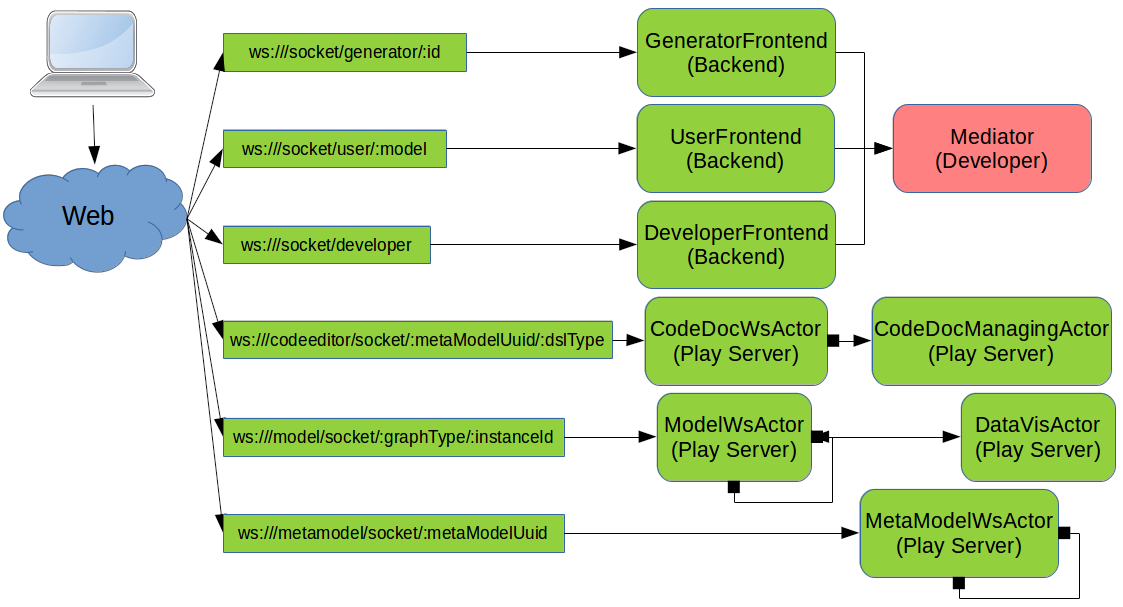
\includegraphics[width=5in]{figures/actor_play_before.png}
    \caption{Ausgangszustand - Websockets}
    \label{fig:ZETA_WS_OLD}
\end{figure}

\subsection{SprayParser}

Der \textit{SprayParser} ist Teil des \textit{Play Servers} und ist verantwortlich dafür die Definitionen der textuellen \acp{dsl} aus dem \textit{Code-Editor} in ein internes Modell zu überführen. Dieses Modell wird genutzt um in einem internen Generator die Konfiguration in JavaScript für den graphischen Editor der Modell Instanzen zu erzeugen. Die Klasse des \textit{SprayParser} besteht im Wesentlichen aus drei verschiedenen aufeinander aufbauenden Parsern für die textuellen \acp{dsl} \textit{Style}, \textit{Spray} und \textit{Diagram}. Weitere deutlich kleinere Parser befinden sich in den unterschiedlichen Modell Klassen des \textit{SprayParsers}. Die textuellen \acp{dsl} sind intern aber auch untereinander hierarchisch aufgebaut. Dabei hängt die \textit{Spray} Sprache von der \textit{Style} Sprache und die \textit{Diagram} Sprache von der \textit{Spray} Sprache und dem Meta Modell ab. Aus diesem Grund benötigen die unterschiedlichen Parser des \textit{SprayParsers} die Ergebnisse der anderen Parser. Somit müssen die Parser in einer bestimmten Reihenfolge aufgerufen werden. Außerdem wird zu diesem Zweck innerhalb des \textit{SprayParsers} ein Cache mit dem Ergebnis der einzelnen Parser vorgehalten. Dieser Cache hat auch noch die Aufgabe die Hierarchien einzelner Elemente innerhalb der textuellen \acp{dsl} aufzulösen. Der Cache wird aber auch noch zusätzlich für die kleineren Parser in den Modell Klassen des \textit{SprayParsers} und dem Generator für die JavaScript Dateien des graphischen Editors verwendet.

\subsection{Generator}
\label{sec:INITIAL_GENERATOR}

In dem Scala Projekt existieren neben dem \textit{Play Server} auch eine Reihe von weiteren Diensten, die unter dem \textit{backend} Unterprojekt zusammengefasst sind. Die Hauptaufgabe des \textit{Backend} Unterprojekts ist es, die Ausführung der Generatoren zu verwalten. Zum \textit{Backend} gehört wie in Abbildung~\ref{fig:ZETA_ARCH_OLD} auf Seite~\pageref{fig:ZETA_ARCH_OLD} zu sehen der \textit{B1}, \textit{Developers} und \textit{Workers} Dienst. Diese Dienste kommunizieren über ein \textit{Actor System} miteinander und sind zusätzlich als \textit{Akka Cluster} konfiguriert. Ein \textit{Akka Cluster} ermöglicht es, die \textit{Akka Aktoren} angefangen über mehrere Prozesse, über mehreren Computern und bis zu mehreren Regionen (wie z.B. Rechenzentren) zu skalieren. Das \textit{Akka Framework} mit den \textit{Akka Actoren} und dem \textit{Akka Cluster} sind Teil der \textit{Lightbend Plattform} \cite{akka}. Innerhalb des \textit{Actor Clusters} kommt eine Vielzahl von \textit{Akka Actoren} in den jeweiligen Diensten zum Einsatz. Eine Übersicht der einzelnen Actoren und ihre Kommunikationswege kann in Abbildung~\ref{fig:ZETA_ACTOR_OLD} auf Seite~\pageref{fig:ZETA_ACTOR_OLD} eingesehen werden. Dabei haben die Actoren, die innerhalb des \textit{Play Servers} ausgeführt werden, eine grüne Hintergrundfarbe und die Actoren der verschiedenen Dienste aus dem \textit{Backend} Unterprojekt haben entsprechend ihrem Dienst eine Hintergrundfarbe. Zusätzlich steht noch bei den Actoren des \textit{Backend} Unterprojekts in Klammern der entsprechende Unterordner bzw. Dienst. Die durchgezogenen Linien bei den Verbindungen zwischen den Actoren repräsentieren eine neu gesendete Nachricht. Währenddessen eine gestrichelte Linie die Weiterleitung einer Nachricht repräsentiert. Zusätzlich hat der \textit{WorkQueue} und der \textit{Master} Actor ein anderes Symbol aufgrund ihrer Sonderfunktion als \textit{Persistent Actor}.

\begin{figure}
    \centering
    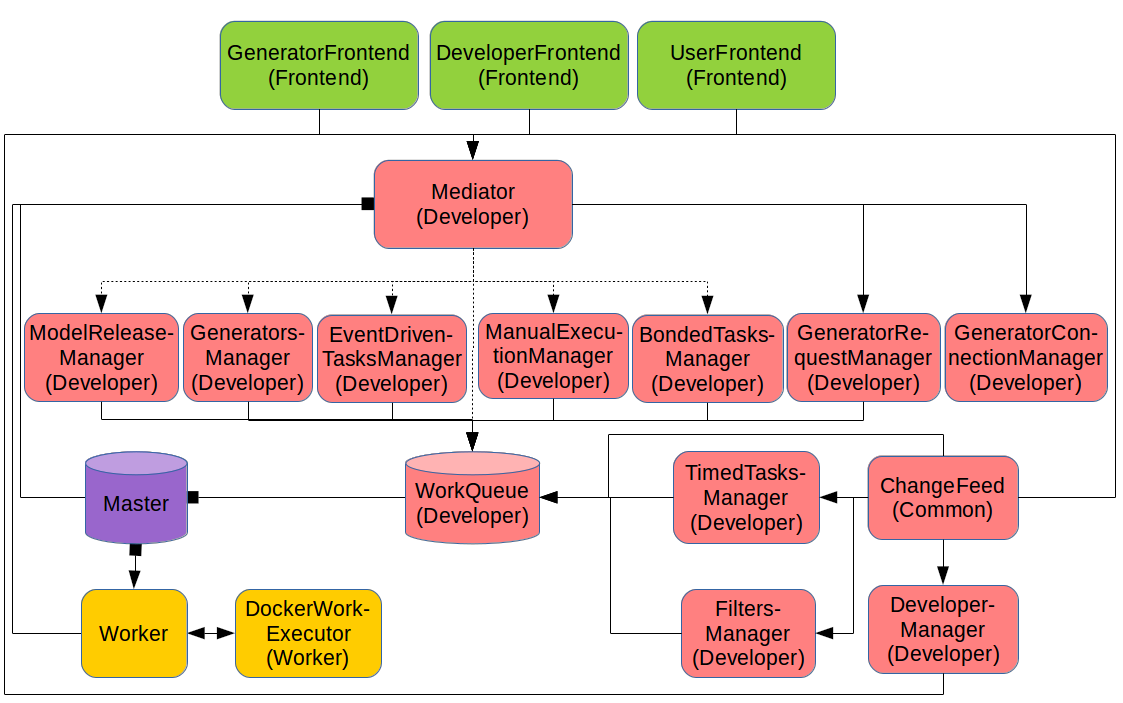
\includegraphics[width=5in]{figures/actor_backend_before.png}
    \caption{Ausgangszustand - Actor Kommunikation}
    \label{fig:ZETA_ACTOR_OLD}
\end{figure}

\begin{sloppypar}
Eine wichtige Funktion der \textit{Akka Actoren} ist ihre Fehlertoleranz \cite{akka_fault_tolerance}. Dabei fungiert ein Actor als \textit{Supervisor} für seine gestarteten Actoren und diese Actoren werden auch Kind Actoren genannt. Somit ergibt sich für die Aktoren zwingend eine hierarchische Struktur, wobei die Actoren auf Exceptions ihrer Kind Actoren reagieren. Die Standard Strategie für Actoren sieht vor, bis auf ein paar Akka interne \textit{Exceptions} den Kind Actor bei einer \textit{Exception} neu zu starten. Alle weiteren Möglichkeiten, wie z.B. ein \textit{Error}, werden auf die nächst höhere Ebene der Hierarchie eskaliert. Die Hierarchie der Actoren in den verschiedenen Diensten des \textit{Actor Clusters} von \textit{Zeta} kann in Abbildung~\ref{fig:ZETA_HIERACHY_OLD} auf Seite~\pageref{fig:ZETA_HIERACHY_OLD} eingesehen werden. Dabei startet z.B. der \textit{Developers} Dienst nur den \textit{Mediator} und den \textit{DeveloperManager} als Top-Level Actor und sämtliche Manager und die \textit{WorkQueue} Actoren werden als Kind Actoren gestartet. Beim \textit{Workers} Dienst wiederum werden alle Actoren als Top-Level Actor gestartet und zusätzlich hat der \textit{Worker} Actor noch eine angepasste \textit{Supervisor Strategy}.
\end{sloppypar}

Ein \textit{Akka Cluster} besteht im Wesentlichen aus \textit{Seed} Nodes und den regurlären \textit{Akka Nodes} \cite{akka_cluster}. Dabei übernehmen die \textit{Seeds} die Aufgabe neue Teilnehmer des Clusters entgegenzunehmen und auch die \textit{Seeds} selbst nutzen die \textit{Seeds} um dem \textit{Akka Cluster} beizutreten. Eine Node ist ein logischer Teilnehmer des Clusters und wird über die Kombination aus Hostname, Port und \textit{UID} identifiziert. Ein \textit{UID} wird einmalig beim Starten einer Node erstellt und verhindert, dass bei einem \textit{Remote Death} eine Node erneut dem Cluster beitreten kann. Das Konzept hinter den Verteilten Workern von \textit{Zeta} basiert auf einem \textit{Worker-Pull} Pattern \cite{akka_worker_pull}. Dabei nehmen die Master die eigentlichen zu bearbeitenden Aufgaben entgegen und die Worker fragen beim Master nach Arbeit. Bei \textit{Zeta} übernimmt der\textit{B1} Dienst zum einen die Aufgabe der \textit{Seed} Node und des Masters. Zusätzlich kommt noch ein \textit{Developers} Dienst zum Einsatz. Innerhalb des \textit{Developers} Dienstes werden sämtliche Anfragen der Websockets des \textit{Play Servers} über die Frontend Actoren entgegen genommen. Dabei wandeln verschiedenen Actoren wie z.B. \textit{GeneratorManager} innerhalb des \textit{Developers} Diensts die Anfragen in sogenannte \textit{Jobs} um und befüllen damit die Warteschlange des \textit{WorkQueue} Actors. Neben den Anfragen aus den Websockets des \textit{Play Servers} nimmt innerhalb des \textit{Developers} Dienstes der \textit{ChangeFeed} Actor Datenbank Änderungen über den \textit{Change Feed} des \textit{Couchbase Sync Gateways} entgegen. Daraufhin sendet der \textit{ChangeFeed} Actor die über den Websocket empfangenen Datenbank Änderungen an sämtliche Actoren des \textit{Developers} Dienstes. Jedoch werden die Nachrichten nur von einem Bruchteil der Actoren auch wirklich verarbeitet und aus diesem Grund sind in Abbildung~\ref{fig:ZETA_ACTOR_OLD} auf Seite~\pageref{fig:ZETA_ACTOR_OLD} auch nur wenige Actoren mit dem \textit{ChangeFeed} Actor verbunden.

\begin{figure}
    \centering
    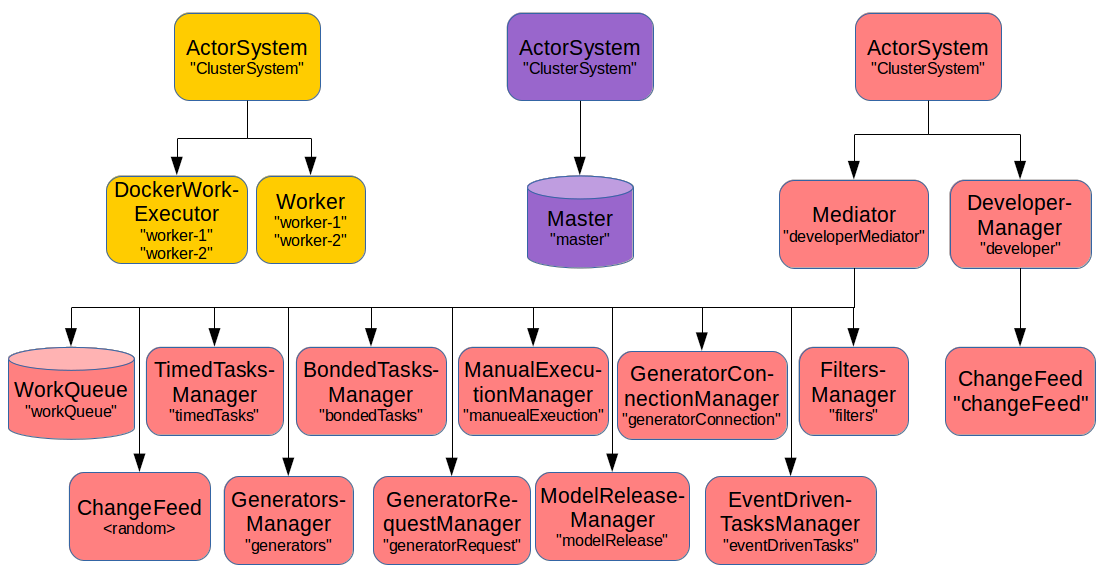
\includegraphics[width=5in]{figures/actor_hierachy_before.png}
    \caption{Ausgangszustand - Actor Hierachie}
    \label{fig:ZETA_HIERACHY_OLD}
\end{figure}

Der \textit{Workers} Dienst ist schlussendlich für die Ausführung der verschiedenen Generatoren per \textit{Docker} zuständig. Dabei wird entsprechend für einen Generator ein neuer \textit{Docker Container} aus den zuvor gebauten \textit{Docker Images} erzeugt und gestartet. Der Generator Container wird beim Start mit in das \textit{Docker Compose} Netzwerk aufgenommen. Mit diesem Zugriff und den übergebenen Parametern wie z.B. dem \textit{Sync Gateway} Sitzungsschlüssel ist der Generator in der Lage, bei der ersten Ausführung sich mit einem Beispiel Programmcode für den entsprechenden Generator zu erstellen. Danach kann der eigentliche Generator in einer separaten Ausführung eines neuen \textit{Docker Containers} ausgeführt werden. Zu diesem Zweck werden innerhalb des Generators über die ID des Generators die Dateien mit den Transformationsregeln von der \textit{Couchbase Datenbank} geladen. Der Inhalt der Dateien wird nun per \textit{Toolbox} des Scala Compilers zur Laufzeit zu einem Transformer kompiliert und mit den Daten einer Modell Instanz ausgeführt. Dabei werde die Daten der Modell Instanz in Form der Datenbank \textit{Entity} an den Transformer übergeben. Grundsätzlich sind die Generatoren in \textit{Zeta} in \textit{Basic-}, \textit{Specific-}, \textit{File-} und \textit{Remote-Generator} unterteilt. Der \textit{Basic-Generator} ist ein vom Meta Modell unabhängiger Generator und der \textit{Specific-Generator} ist für ein bestimmtes Meta Modell. Der \textit{File-Generator} demonstriert das Erstellen von Dateien innerhalb eines Generators und der \textit{Remote-Generator} demonstriert das Ausführen eines weiteren Generators per Websocket vom \textit{Play Server}. Neben diesen Generatoren werden auch der \textit{Filter} und das \textit{MetaModelRelease} vom \textit{Workers} Dienst als eigenständiger \textit{Docker Container} ausgeführt. Beim \textit{Filter} werden in Scala erstellte Regeln zur Filterung der Modell Instanzen wie bei den Generatoren über die Scala \textit{Toolbox} ausgeführt. Das Ergebnis wird zusammen mit dem \textit{Filter} gespeichert. Beim \textit{MetaModelRelease} wird der aktuelle Stand aus \textit{Code-Editor} und \textit{MetaModel-Editor} genommen und unter einer neuen Version abgespeichert.

\subsection{Datenbanken}

Aktuell werden innerhalb von \textit{Zeta} mehrere Datenbanken eingesetzt. Zum einen eine \textit{MongoDB}, aber auch eine \textit{Couchbase Server} mit davor geschaltetem \textit{Sync Gateway}. Beide Datenbank Systeme sind \textit{NoSQL} Datenbanken und arbeiten mit \ac{json} Dokumente. Dabei bieten beide Datenbank Systeme nicht wie z.B. bei relationalen Datenbanken eine offen gehaltene Verbindung, sondern eine über \ac{http} laufende \ac{rest} \acp{api}. Auf der einen Seite wurde die \textit{MongoDB} in der Vergangenheit primär in \textit{Zeta} verwendet. Wie in der Abbildung~\ref{fig:ZETA_ARCH_OLD} auf Seite~\pageref{fig:ZETA_ARCH_OLD} zu sehen ist, wird die \textit{MongoDb} nur vom \textit{Play Server} verwendet und ist nicht öffentlich über den \textit{Proxy} Dienst zugänglich. Inzwischen wird die \textit{Mongodb} innerhalb des \textit{Play Servers} nur noch für die Persistierung der Daten aus dem Websocket des \textit{Code-Editors} verwendet.

Auf der anderen Seite wird die \textit{Couchbase Datenbank} mit dem \textit{Sync Gateway}, wie in Abbildung~\ref{fig:ZETA_ARCH_OLD} auf Seite~\pageref{fig:ZETA_ARCH_OLD} zusehen, von fast allen Diensten innerhalb von \textit{Zeta} verwendet. Zudem erfolgen auch während der Ausführung der Generatoren mehrere Zugriffe auf die Datenbank. Dadurch ist die \textit{Couchbase Datenbank} primär für die Persistierung der angefallenen Daten innerhalb von \textit{Zeta} zuständig. Zum Teil haben die Daten aus dem \textit{Couchbase Server} Überlappungen mit den Daten in der \textit{Mongodb}. Das vor der \textit{Couchbase Datenbank} geschaltete \textit{Sync Gateway} ist zusätzlich auch öffentlich über den \textit{Proxy} Dienst erreichbar. Dieser externe Zugriff auf das \textit{Sync Gateway} wird dazu genutzt um vom Browser aus innerhalb der \textit{Webbapp} auf die Datenbank zuzugreifen. Speziell der \textit{Change Feed} des \textit{Sync Gateways} wird einmal innerhalb der \textit{Webapp} im Browser und zudem mehrfach von den Actoren des \textit{Akka Clusters} des \textit{Backend} Projekts genutzt.


\chapter{Review}
\label{ch:REVIEW}

Nachdem im Kapitel~\ref{ch:INITIAL} zuvor die Architektur von \textit{Zeta} im Ausganszustand beschrieben worden ist, werden in diesem Kapitel die einzelnen Teile der Architektur kritisch betrachtet. Dabei werden die vorhandenen Lösungen auf die Nutzung von Entwurfsmustern oder auch Design Prinzipien bewertet. Aber auch die Nutzung weiterer Entwurfsmuster wird evaluiert. Die Architektur wird zusätzlich auf das vorhanden sein von Anti-Pattern untersucht. Für etwaige kritische Teile werden jeweils unterschiedliche Lösungsvarianten erörtert.

Dieses Kapitel beginnt mit der \textit{Docker Compose} Umgebung und der Konfiguration der einzelnen Dienste. Drauf folgt eine Betrachtung der verschiedenen Unterprojekte innerhalb des Scala Projekts. Abgeschlossen wird das Ganze mit der Datenbank von Couchbase.

\section{Docker Compose Umgebung}

In diesem Abschnitt wird genauer auf die Konfiguration der Laufzeitumgebung für \textit{Zeta} per \textit{Docker Compose} eingegangen \cite{zeta_docker_compose}. Entsprechend werden die Konfiguration der jeweiligen Dienste innerhalb von \textit{Docker} Compose analysiert, aber auch die eigens für \textit{Zeta} definierten \textit{Docker Images}. Grundlage dieser Analyse sind die offiziellen Guidelines für \textit{Docker Compose} im Produktivbetrieb, die Best Practices zur Software Entwicklung mit \textit{Docker}, die Best Practices zur Erstellung eines \textit{Dockerfiles} und die Security by Design Prinzipien von \ac{owasp} \cite{docker_best_practices,docker_compose_production,dockerfile_best_practices,owasp_security_by_design}. Die Security by Design Prinzipien von \ac{owasp} kommen bei der Betrachtung der \textit{Docker Compose} Umgebung zum Einsatz, da diese Sammlung an Prinzipien sich zum Ziel gesetzt hat, sichere Architektur bei Erstellung von Webapplikation zu erreichen.

\subsection{Maßgeschneidertes Proxy Image}

Beginnend mit dem \textit{Proxy} als ersten Dienst in der \textit{Docker Compose} Konfiguration. Beim \textit{Proxy} Dienst wird eigens ein \textit{Docker Image} über ein \textit{Dockerfile} definiert. Entsprechend der Best Practices von \textit{Docker} sollte eine genaue Version beim genutzten Image von \textit{Nginx} angegeben werden, anstelle sich auf neusten Stand über das latest als Standard Tag zu verlassen. Somit wird eine Inkompatibilität durch Breaking Changes bei einer neuen Hauptversion verhindert und alle Entwickler nutzen dieselbe Version von \textit{Nginx} um auf allen Systemen die gleiche Umgebung zu haben.

Einer der Best Practises besagt die Gesamtgröße von \textit{Docker Images} und die Anzahl der Layer innerhalb eines Image sollten möglichst klein gehalten werden. Zu diesem Zweck sollten über die Definitionen in einem \textit{Dockerfile} nur die nötigsten Abhängigkeiten enthalten sein und auf unnötige Pakete sollte verzichtet werden. Zusätzlich ist auch die Größe eines \textit{Docker Image} immer ein relevanter Punkt. Der \textit{Proxy} Dienst nutzt das Standard \textit{Nginx} Image. Jedoch ist \textit{Nginx} auch in einer minimallen Variante mit \textit{Alpine} als Basis Image vorhanden und hat im Vergleich zum Standard Image nur ein Bruchteil der Größe. Die \textit{Alpine} Variante ist nicht mit sämtlich möglichen Szenarien kompatibel. Dennoch sollte die \textit{Alpine} Variante aufgrund kürzerer Downloadzeiten, Schonung der Bandbreite, schnelleres Starten von \textit{Docker Containern} und allgemein weniger Ressourcenverbrauch des Computers bevorzugt werden.

Weiterhin wird im \textit{Dockerfile} nur eine einzige Datei in das Image kopiert. Bei dieser Datei handelt es sich um die Konfigurationsdatei der \textit{Virtual Hosts} innerhalb von \textit{Nginx}. Die Konfigurationsdatei von \textit{Nginx} kann auf einem lokalen Entwicklungssystem auch direkt per \textit{Bind Mount} eingebunden werden. Somit würde das Erzeugen des \textit{Docker Images} für den \textit{Proxy} Dienst überflüssig. Auch bei Änderungen müsste im äußersten Fall der Dienst nur neugestartet werden oder im Fall von \textit{Nginx} würde ein Steuersignal zum erneuten Laden der Konfigurationsdateien ausreichen. Für den produktiven Betrieb sollten jedoch \textit{Bind Mounts} nicht genutzt werden, um die Konfigurationsdatei vor Veränderung zu schützen. Zur Laufzeit von \textit{Docker Compose} werden die Abhängigkeiten zu den anderen Diensten wie z.B. dem \textit{Play Server} über \textit{Docker Links} aufgelöst. Zusätzlich wird noch der Treiber für das Logging der Ausgaben deaktiviert. \textit{Docker Compose} ermöglich es jedoch zur Laufzeit die Logs gezielt auf einen einzigen oder mehrere ausgewählte Dienste zu filtern und somit ist eine Deaktivierung des Logging Treibers nicht notwendig.

\subsection{Couchbase Server und Sync Gateway}

Beim dem nächsten Dienst, dem \textit{Couchbase Server}, sieht die Konfiguration mit extra \textit{Dockerfile} ähnlich wie beim \textit{Proxy} Dienst aus. Beim Verweis auf \textit{Docker Image} des \textit{Couchbase Servers} wird keine Version angegeben und somit wird immer die aktuellste Enterprise Variante des \textit{Couchbase Servers} bei der ersten Ausführung bezogen. Ein Wechsel auf die Community Variante mit der genauen \textit{Couchbase Server} Version würde sich hier anbieten. Die Nutzung einer \textit{Alpine} Variante ist aktuell nicht möglich, da offiziell eine solche Variante von Couchbase nicht angeboten wird und auch zukünftig nicht geplant ist \cite{couchbase_alpine}. Auch scheint eine \textit{Alpine} Variante kein triviales Unterfangen zu sein, da bis zum aktuellen Zeitpunkt noch kein Image mit dieser Variante aus der Community zu Verfügung gestellt wurde. In diesem \textit{Dockerfile} wird anstelle einer Konfigurationsdatei wie im \textit{Proxy} Dienst jedoch ein Shell-Script in das eigene \textit{Docker Image} kopiert. Dies ist notwendig damit die Datenbank und ein Benutzer mit einem Passwort initialisiert wird, da das offizielle Image diese Funktion von sich aus nicht bietet.

Anstelle das Ganze mit einem \textit{Dockerfile} zu lösen, kann der ursprüngliche \textit{ENTRYPOINT} in \textit{Docker Compose} z.B. durch einen \textit{Bind Mount} überschrieben werden und die einhergehende Anpassung des Pfads zum \textit{ENTRYPOINT} könnte ganz weggelassen werden. Damit lässt sich auch beim Dienst für den \textit{Couchbase Server} der zusätzliche Build Vorgang für das \textit{Docker Image} umgehen. Des Weiteren ist eine Datenbank von Natur aus zustandsbehaftet und auch der \textit{Couchbase Server} schreibt die Daten der Datenbanken in ein bestimmtes Verzeichnis. Aus diesem Grund wird in \textit{Docker Compose} zur Persistierung das Verzeichnis mit den Daten auf das Hostsystem gemapped. Dabei wird dieses Verzeichnis global in das Hauptverzeichnis gemapped, anstelle es auf das lokale Verzeichnis von \textit{Docker Compose} zu mappen. Auch einige Ports des \textit{Couchbase Servers} sind für den Zugriff vom Hostsystem und extern freigegeben. Für den Betrieb von \textit{Zeta} ist dies nicht notwendig, da die Zugriffe von den verschiedenen Diensten über die internen Links von \textit{Docker} erfolgen und der Rest über den Reverse-Proxy erreichbar ist. Zum Debuggen oder zu Testzwecken kann ein Zugriff über das Hostsystem erfolgen, aber ein externer Zugriff sollte aufgrund des Prinzip Secure-by-Default untersagt sein, um nicht schlussendlich diese Konfiguration für den produktiven Betrieb zu übernehmen.

Beim \textit{Database} Dienst wird für das \textit{Couchbase Sync Gateway} auch wieder ein \textit{Dockerfile} mit einer Konfigurationsdatei, einem eigenen \textit{ENTRYPOINT} und der lokalen sowie externen Freigabe einiger Ports per \textit{Docker Compose} gearbeitet. Dazu sei zu erwähnen, dass beim \textit{Docker Image} die Community Variante mit einer spezifischen Version genutzt wird. Auch beim \textit{Sync Gateway} wird keine \textit{Alpine} Variante, weder von offizieller Seite, noch aus der Community angeboten. Außerdem werden die freigegebenen Ports aufgrund der Links per \textit{Docker Compose} nicht für den Betrieb von \textit{Zeta} benötigt und der Zugriff sollte entsprechend auf das Hostsystem begrenzt sein. Auch um einen externen Zugriff auf den Port der Admin \ac{rest} \ac{api} in jedem Fall zu unterbinden.

\subsection{Node.js Server der Webapp mit Bower}

Der \textit{Webapp} Dienst nutzt auch ein eigens erstelltes \textit{Dockerfile} und ist ein \ac{npm} Projekt für \textit{Node.js}. Dabei wird auf das offizielle \textit{Node.js} Image mit einer bestimmten Version aufgebaut. Bei der Version wird entsprechend des Semantic Versionings aber nur ein Minor Release angeben und nicht einschließlich des Patch Release \cite{semver}. Für das offizielle \textit{Node.js} Image steht auch eine minimalisierte \textit{Alpine} Variante zur Verfügung. Im weiteren Verlauf des \textit{Dockerfiles} geht es primär um den Download der über \ac{npm} und \textit{Bower} definierten Abhängigkeiten. Zum einen sollte statt \ac{npm} der \textit{Yarn} Pakete Manager genutzt werden. \textit{Yarn} nutzt die offiziellen Server von \ac{npm} und unterstützt auch dasselbe Format zum Definieren der Abhängigkeiten. Aber der Prozess des Auflösen und Downloaden der Abhängigkeiten wurde gegenüber \ac{npm} stark verbessert und \textit{Yarn} steht inzwischen sogar in der \textit{Alpine} Variante des \textit{Node.js} Images zur Verfügung. Zum anderen verursacht die Nutzung von \textit{Bower} als weiterer Pakete Manager aufgrund der \textit{Polymer} Bibliothek eine höhere Komplexität. Inzwischen sind immer mehr Pakete direkt per \ac{npm} verfügbar und die Nutzung eines weiteren Paket Managers speziell für webbasierte Bibliotheken oder Frameworks ist immer seltener von Nöten. Auch das \textit{Polymer} Projekt hat diesen Veränderung inzwischen wahrgenommen und wird in naher Zukunft mit der nächsten Major Version von einem \textit{Bower} Projekt auf ein \ac{npm} Projekt wechseln \cite{polymer3_preview}. Somit lässt sich hier auch die Komplexität nach dem \ac{kiss} Prinzip weiter verringern. Eine alternativer Ansatz der jetzt schon möglich ist, ist das Auflösen per \textit{Bower} über einen \textit{Hook} in den regulären Installationsprozess von \ac{npm} bzw. \textit{Yarn} zu integrieren. Des Weiteren sind die genauen Befehle und ihre Reihenfolge der Pakete Manager nur im \textit{Dockerfile} definiert und es muss für jede Änderung an den Abhängigkeiten erneut ein \textit{Docker Image} erzeugt werden. Durch die Lösung mit dem \textit{Hook} kann nach dem \ac{soc} Prinzip das Auflösen der Abhängigkeiten zurück in das \ac{npm} Projekt verlagert werden und nun sogar ohne die Nutzung von \textit{Docker} ausgeführt werden. Somit müsste auch das Image während der Entwicklung von \textit{Zeta} nicht bei jeder Änderung an den Abhängigkeiten neu erzeugt werden und könnte durch einen Neustart des \textit{Webapp} Diensts erfolgen. Schlussendlich werden im \textit{Dockerfile} noch alle Dateien der \textit{Webapp} in das Image kopiert.

Zur Laufzeit wird dann per \textit{Docker Compose} erneut der Inhalt der \textit{Webapp} in den \textit{Docker Container} per \textit{Bind Mount} gemapped. Das Mapping der \textit{Webapp} ist notwendig um nicht nach jeder Dateiänderung das Image neu zu erzeugen und der Einsatz von \textit{Browsersync} wäre ansonsten überflüssig. Des Weiteren werden sogenannte \textit{Docker Volumes} auf die Verzeichnisse mit den heruntergeladenen Paketen der Abhängigkeiten von \ac{npm} und \textit{Bower} gemountet. Dabei ist bei der aktuellen Konfiguration zu beachten, dass beim ersten Start des \textit{Webapp} Diensts das Volume noch gänzlich leer ist und anders als beim \textit{Bind Mount} wird der Inhalt des Verzeichnis aus dem Container in das Volume geschrieben \cite{docker_storage_tips}. Entsprechend werden hier die Daten der Pakete in das Volume geschrieben. Bei einem zweiten Start des \textit{Webapp} Diensts ist das Volume nicht mehr leer und verhält sich nun wie ein \textit{Bind Mount}. Der Container kann über das Zielverzeichnis auf den Inhalt des Volumes oder \textit{Bind Mounts} zugreifen. Etwaiger Inhalt des Zielverzeichnisses, der z.B. beim Erzeugen des Image erstellt wurde, wird nicht überschrieben, aber wird vom Inhalt des Volumes oder \textit{Bind Mounts} überlagert. Dies führt z.B. zu dem Effekt beim \textit{Webapp} Dienst, dass zu Beginn alles normal funktioniert. Aber sobald aufgrund von Änderungen an den Abhängigkeiten das Image neu erzeugt wird, wird zur Laufzeit des Containers der Inhalt aus dem Volume mit den alten Abhängigkeiten genutzt und nicht die veränderten Abhängigkeiten aus dem Image. Des Weiteren werden zur Laufzeit sämtliche Ports zusätzlich extern freigegeben. Dies ist zum Betrieb von \textit{Zeta} nicht notwendig und sollte wie schon zuvor auf das Hostsystem begrenzt sein. Falls nicht zwingend notwendig, sollten diese Port-Freigaben gänzlich entfernt werden. Zusätzlich wird zur Laufzeit ein \textit{Workingdir} gesetzt und mit den zuvor erwähnten Änderung beim Auflösen der Anhängigkeiten ist das eigene \textit{Docker Image} nicht länger notwendig. Somit ist der aktuelle Build Vorgang für das \textit{Docker Image} des \textit{Webapp} Diensts überflüssig. Weiterhin wird auch der Treiber für das Logging der Standardausgabe des Containers wieder innerhalb von \textit{Docker Compose} deaktiviert.

\subsection{MongoDB Dienst}

Für den \textit{Mongodb} Dienst wird das offiziele \textit{Docker Image} und kein eigenes Image muss noch zusätzlich erzeugen werden. Zusätzlich wird auch eine Version für das Image mit angegeben. Jedoch ist die angegebene Version nur ein Major Release und kein Patch Release. Von offizieler Seite gibt es keine \textit{Alpine} Variante für das \textit{Mongo} Image. Aber aus der Community werden einige \textit{Docker Images} auf Basis von \textit{Alpine} für \textit{Mongo} bereitgestellt. Jedoch kommt keines dieser Images an den Funktionsumfang und die Qualität des offiziellen \textit{Mongo} Image heran. Entweder ist der Bezug einer bestimmten Version des \textit{Mongo} Server nicht möglich oder die Images haben keine automatische Einrichtung eines Benutzers mit Passwort. Aktuell wird die Funktion zur Einrichtung eines Benutzers mit Passwort nicht für den \textit{Mongodb} Dienst in \textit{Zeta} genutzt und somit ist Standardmäßig ein anonymer Zugriff auf die Datenbank möglich.  Das Verzeichnis, in dem der \textit{Mongo} Server die Daten schreibt, wird per \textit{Bind Mount} auf das Hostsystem gemapped. Jedoch wird auch diesmal wieder dafür ein Verzeichnis im globalen Stammverzeichnis genutzt und nicht ein lokales Verzeichnis. Desweiteren wird auch der Port extern freigegeben. Dies ist zum Betrieb von \textit{Zeta} nicht notwendig und sollte nach dem Prinzip Secure-by-Default wie zuvor auf das Hostsystem begrenzt sein. Schlussendlich ist auch bei diesem Dienst der Treiber für das Logging deaktiviert worden und sollte aus demselben Grund wie zuvor die Standard Einstellung benutzen.

\subsection{Images per sbt-native-packager}

Die restlichen Dienste in der \textit{Docker Compose} Konfiguration wie der \textit{Play Server} oder \textit{Workers} bauen auf eigene \textit{Docker Images} auf. Dabei werden diese \textit{Docker Images} nicht von \textit{Docker Compose} erzeugt, sondern müssen händisch vor dem ersten Start von \textit{Docker Compose} über das zuvor erwähnte Setupscript aus dem Programmcode~\ref{lst:ZETA_SETUP} auf Seite~\pageref{lst:ZETA_SETUP} erzeugt werden. Die Erzeugung der Images erfolgt pro \ac{sbt} Unterprojekt über den Task \textit{docker:publishLocal} des \textit{sbt-native-packager} Plugins. Das Plugin muss innerhalb von \ac{sbt} in den entsprechenden Unterprojekten per \textit{JavaAppPackaging} aktiviert sein. Jedoch wie in der List der genutzten \ac{sbt} Plugins aus der Tabelle~\ref{tab:ZETA_SBT_OLD} auf Seite~\pageref{tab:ZETA_SBT_OLD} zusehen ist, ist der \textit{sbt-native-packager} nicht in \textit{Zeta} enthalten. Bei einer genaueren Analyse der genutzten \ac{sbt} Plugins stellt sich heraus, dass der \textit{sbt-native-packager} eine Abgängigkeit des \ac{sbt} Plugin für das \textit{Play Framework} ist \cite{play_sbt_plugin_packager}. Nun nutzt \textit{Zeta} die Funktionalität des \textit{sbt-native-packager} außerhalb des Unterprojekts für den \textit{Play Server} und sollte aus diesem Grund auch explizit bei den genutzten \ac{sbt} Plugins aufgeführt werden.

Des Weiteren müssen während der Entwicklung von \textit{Zeta} nach jeder Änderungen am Programmcode, z.B. am \textit{Play Server} oder dem \textit{Workers} Dienst, die \textit{Docker Images} erneut erzeugt werden, da in den per \ac{sbt} erzeugten \textit{Docker Images} nur noch die Java Archive mit den kompilierten Scala Dateien enthalten sind. Aufgrund des fehlenden Build-Systems innerhalb der Images kann auch nicht zur Laufzeit der Programmcode in den \textit{Docker Container} gemapped werden. Die Erzeugung der Images per \ac{sbt} ist auf den Einsatz in einem Produktivsystem optimiert, aber erzeugt zusätzlichen Overhead bei Nutzung als Entwicklungssystem.

Zusätzlich sollte beim Einsatz von \textit{Docker Compose} ein Projekt nach dem \ac{kiss} Prinzip aufgesetzt werden. Entsprechend sollte beim Aufsetzen eines Entwicklersystems für \textit{Zeta} nur das Auschecken der aktuellen Version aus der Versionsverwaltung und das anschließende Ausführen von \textit{Docker Compose} notwendig sein. Ein alternativer Ansatz ist die Ausführung der Unterprojekte über den \ac{sbt} Launcher. Im Fall des \textit{Play Servers} wird das \textit{Play Framework} bei der Ausführung über den Launcher im Entwicklungsmodus und nicht wie in der aktuellen Lösung im Produktivmodus ausgeführt. Dabei unterstützt das \textit{Play Framework} den Entwickler durch automatisches Erkennen von geänderten Dateien und führt einen Incremental Build Vorgang aus. Die Erkennung von Änderungen wird bei jedem Aufruf von z.B. eines \ac{html} Dokuments oder einem Asset im Hintergrund ausgeführt und entstandene Fehler beim Build Vorgang werden dem Entwickler direkt als Webseite zurückgegeben. Damit benötigt der \textit{Play Server} gegenüber den weiteren Diensten wie z.B. dem \textit{Workers} Dienst nicht einmal einen Neustart um den Build Vorgang auszuführen.

\subsection{Container abhängige Konfiguration}

Die verschiedenen Dienste wie der \textit{Play Server} oder der \textit{Workers} Dienst nutzen in der \textit{Docker Compose} Konfiguration entweder Umgebungsvariablen oder Übergabeparameter um \textit{Docker} spezifische Einstellung wie z.B. Hostnamen zu den anderen \textit{Docker Container} festzulegen. Dies wird aber bei weitem nicht für alle Docker spezifischen Einstellungen gemacht. Einstellungen wie Hostnamen oder Zugangsdaten für die verschiedenen Datenbank Dienste sind in Konfigurationsdateien oder Scala Klassen hartcodiert \cite{zeta_docker_mongodb,zeta_docker_couchbase_admin,zeta_docker_couchbase_public,zeta_docker_play_seeds,zeta_docker_remote_api}. Die Scala Projekte sollten unabhängig von \textit{Docker} konfiguriert sein, um keine Bindung an \textit{Docker} zu verursachen. Die Information wie z.B. Hostnamen zum Zusammenspiel der verschiedenen Dienste sollte von außen an die Dienste herangetragen werden. Dies ermöglich auch z.B. die Umbenennung eines Dienst in der \textit{Docker Compose} Konfiguration ohne das zusätzlich eine einzige Zeile am Programmcode eines der Dienstes geändert werden muss.

Des Weiteren ist die Nutzung von Umgebungsvariablen und Programmparametern in \textit{Docker Compose} für sicherheitsrelevante Informationen wie z.B. Zugangsdaten in einem lokalen Entwicklungssystem ausreichend. In einem Produktivsystem sollte die Nutzung derselben für sicherheitsrelevante Information durch \textit{Docker Secrets} ersetzt werden. Umgebungsvariablen und auch Programmparameter können von Benutzern mit den entsprechenden Rechten systemweit ausgelesen werden. Die \textit{Docker Secret} Funktion gehört zum \textit{Docker Swarm} und stellt nur dem freigegebenen Container innerhalb eines \textit{Docker Cluster} die Information über einen sicheren Kanal zur Verfügung.

\subsection{Flexible Skalierung der Dienste}

Mit dem \textit{B1} und \textit{B2} Dienst sind erste Ansätze zur Skalierung der Dienste in der \textit{Docker Compose} Konfiguration vorhanden. Jedoch ist dieser Ansatz mit sehr viel Aufwand bei der Skalierung verbunden, da für einen weiteren Master oder Slave ein neuer Dienst angelegt werden muss und die Konfiguration der bestehenden Dienste angepasst werden muss. \textit{Docker Compose} unterstützt eine Funktion namens Replikation. Dadurch kann in der Konfiguration angegeben werden wie oft ein bestimmter Dienst von \textit{Docker Compose} gestartet werden soll. Als Beispiel kann z.B. ein Dienst namens Master mit fünf Replikationen in \textit{Docker Compose} angelegt werden. Zur Laufzeit von \textit{Docker Compose} sind die Dienste \textit{zeta\_master\_1} bis \textit{zeta\_master\_5} vorhanden. Auf den ersten Blick ist weiterhin die Anpassung der anderen Dienste wie z.B. dem \textit{workers} Dienst notwendig. Jedoch liefert \textit{Docker} per DNS Loadbalancing unter der Adresse \textit{zeta\_master} die IP Adressen aller fünf laufenden Master Dienste. Beim Joinen der Nodes in den \textit{Akka Cluster} müssten alle Adressen und nicht nur die erste Adresse per DNS aufgelöst werden. Dies ermöglicht z.B. in einen Produktivsystem einen skalierbaren \textit{Akka Cluser} ohne zusätzlichen Konfigurationsaufwand. Über einen \textit{Docker Swarm} wäre zusätzlich eine Skalierung über mehrere Computer ohne weiteren Konfigurationsaufwand möglich. Über diesen Mechanismus ist auch eine transparente Skalierung des \textit{Play Server} über mehrere Instanzen möglich.  

Beim Einsatz in einem Entwicklersystem spielt nicht mehr eine möglichst große Skalierung von \textit{Zeta} die Hauptrolle, sondern im Gegensatz dazu soll \textit{Zeta} mit minimalen Overhead und geringem Ressourcenverbrauch ausgeführt werden. Gleichzeitig sollen auch automatische Build Vorgänge und Dienste im speziellen Modus für Entwickler unterstützt werden. Zu diesem Zweck macht es Sinn den einen oder anderen Dienst falls möglich zusammen zu legen. Die Dienste \textit{B1}, \textit{B2}, \textit{developers} und \textit{workers} werden alle aus demselben \textit{Docker Image} bzw. \ac{sbt} Unterprojekt gestartet. Diese Dienste könnten durch das Hinzufügen spezifischer Programmparameter und der Nutzung des \textit{Akka Clusters} sogar innerhalb eines Prozesses derselben JVM gestartet werden. Diese gewonnene Flexibilität ermöglicht zusätzliche Szenarien bei der Skalierung von \textit{Zeta}.

\subsection{Datenzugriffe des Generator Containers}

Neben dem Image für den \textit{Play Server} und den Diensten des \textit{Akka Clusters} werden für den \textit{ScalaFilter} und die vier weiteren \ac{sbt} Unterprojekte der Generatoren noch jeweils ein \textit{Docker Image} erzeugt. Aus dem Image werden zur Laufzeit von \textit{Zeta} neue Container gestartet. Dabei treten diese Container dem privaten \textit{Docker Compose} Netzwerk bei, um einen Zugriff auf den \textit{Play Server} und das \textit{Couchbase Sync Gateway} zu ermöglichen. Zuerst einmal ist der Name des \textit{Docker Compose} Netzwerk in der \textit{DockerWorkExecutor} Klasse hartcodiert und dabei ist der Name abhängig von der \textit{Docker Compose} Konfiguration. Diese Information sollte aufgrund des \ac{soc} Prinzipes von außerhalb an den \textit{workers} Dienst herangetragen werden. Zusätzlich ist der Beitritt zum \textit{Docker Compose} Netzwerk nicht notwendig, da zum einen der \textit{Play Server} und das \textit{Couchbase Sync Gateway} extern über den \textit{Proxy} Dienst erreichbar sind.

Das eigentliche Problem bei dieser Lösung ist jedoch der direkte Zugriff auf das \textit{Couchbase Sync Gateway}. Die Generatoren können ohne Authentifizierung über die Admin \ac{rest} \ac{api} auf die Datenbank zugreifen. Über den \textit{Proxy} Dienst wäre der Zugriff auf die Public \ac{rest} \ac{api} des \textit{Synx Gateways} begrenzt und durch eine Authentifizierung geschützt. In Teilen wird die Public \ac{rest} \ac{api} schon in den Generatoren verwendet und zur Authentifizierung kommt ein Cookie mit einer Session ID für das \textit{Sync Gateway} zum Einsatz. Die Session ID wird hierbei beim Starten des Containers als Programmparameter übergeben.

Inneralb der Generatoren werden die \ac{m2t} Transformationsregeln aus der Datenbank abgefragt. Die Transformationregeln bestehen aus Scala Programmcode und können flexibel eingesetzt werden. Aus diesen Benutzer definierten Transformationsregeln wird ein Transformer kompiliert und ausgeführt. Neben den Daten der Model Instanz bekommt der Transformer eine \ac{api} mit Vollzugriff auf die Datenbank übergeben. Damit kann ein Benutzer über die Transformationsregeln alle Daten auslesen, verändern und löschen. Selbst ohne die Übergabe der \ac{api} hat der Benutzer über die Transformationsregeln weiterhin Vollzugriff auf die Datenbank, da alle an den Container übergebenen Informationen wie Programmparameter, Umgebungsvariablen oder selbst \textit{Docker Secrets} ausgelesen werden können. Der Transformer läuft innerhalb derselben \ac{jvm} und hat auf alle Klassen des Generators Zugriff und kann sich zur Not seinen eigenen Client für das \textit{Sync Gateway} erstellen. Die Integrität von \textit{Zeta} ist durch diese Lösung erheblich geschwächt und sollte grundlegend überdacht werden.

Sämtliche Datenzugriffe der Generatoren sollten wie ein öffentlicher Datenzugriff gehandhabt werden und sollten nach den Prinzipien Least-Privilege und Separation-of-Duties erfolgen. Ein möglicher Lösungsansatz für das Problem wäre eine Partitionierung der Daten in eine Datenbank pro Benutzer. Wobei zusätzlich noch bestimmte Daten für alle Benutzer zugänglich sein müssen. Dies erzeugt zum einen deutlich höheren Verwaltungsaufwand auf Seiten der Datenbankbenutzer und teils weitere schwer absehbare Zusatzaufwände. Desweiten kann der Benutzer aufgrund des frei wählbaren Schemas einer \textit{Couchbase Datenbank} auch Daten in einem für das Back-End ungültigen Schema erzeugen und so weitere schwer vorhersehbare Probleme verursachen.  Ein weiterer Lösungsansatz könnte durch einen indirekten Zugriff auf die Datenbank realisiert werden. Dabei werden die Generatoren von den Datenbank getrennt und  die Zugriffe erfolgen z.B. über die \ac{rest} \ac{api} des \textit{Play Server}. Innerhalb des \textit{Play Server} kann der Datenzugriff für den Generator nur auf die notwendigsten Daten begrenzt werden. Dabei kann eine Session ID für den \textit{Play Server} an die Generatoren übergeben werden, da auch der Transformer nur auf die eingeschränkten Daten eines einzigen Benutzers Zugriff hat. Ein eher klassischer Ansatz wäre es, den Datenaustausch per Interprozesskommunikation über den \textit{DockerWorkExecutor} zu realisieren. Weitere Lösungsansätze sind möglich, aber der entscheidende Faktor ist die Sicherstellung einer streng regulierten und kontrollieren Kommunikation mit dem restlichen Back-End von \textit{Zeta}.

\subsection{Datenbank Fixtures für Generatoren}

Neben den Images für die \textit{Docker Compose} Dienste und den Generatoren wird am Ende des Setupscripts noch ein weiteres \textit{Docker Image} erzeugt. Das \textit{modigen:data} getaufte Image hat zur Aufgabe, während der Ausführung als \textit{Docker Container}, initial einige notwendige Daten für die Generatoren in die \textit{Couchbase Datenbank} zu schreiben. Das ganze muss also zusätzlich zum Setupscript ausgeführt werden, aber erst nachdem \textit{Zeta} durch \textit{Docker Compose} gestartet wurde. Die exakte Dokumentation des Befehls zur Ausführung des Containers ist nur in der Readme enthalten und hat als einzigen Parameter das private Docker Compose Netzwerk von \textit{Zeta}. Die enwickelte Lösung enthält dabei hartcodierte Zugangsdaten zur Public \ac{rest} \ac{api} des \textit{Couchbase Sync Gateways} und hat keinerlei Möglichkeit diese z.B. über Programmparameter oder Umgebungsvariablen von außen zu konfigurieren \cite{zeta_docker_data}. 

Die Lösung baut auf \textit{Node.js} auf und besteht primär aus einem Script zur Erstellung von Einträgen für die vier Generator Images in der Datenbank. Weder in \textit{Webapp} noch in der Generator Verwaltung per \textit{Akka Cluster} ist irgendeine Verwaltung der Generator Images vorhanden. Für die Einträge der Generator Images sind nur lesende Zugriffe vorhanden. Diese Lösung ist schon von der grundsätzlichen Konzeption schwierig. Nach dem \ac{kiss} und \ac{dry} Prinzip wäre eine Lösung in einem der bestehenden Dienste zu bevorzugen. Auch nach dem Prinzip zur Modularisierung wie z.B. dem Prinzip der Hohen Kohäsion würde die Lösung eher in einer der Dienste des \textit{Akka Cluster} zur Verwaltung der Generatoren gehören und nicht in ein eigenes Module. Zusätzlich rechtfertigt der erhöhte Implementierungs-, Build, und Einrichtungsaufwand nicht die gewählte Lösung. Dabei kann das ganze aufgrund der Lesezugriffe mit minimaler Komplexität über eine List innerhalb der Konfiguration oder in diesem Fall sogar hartcodiert gelöst werden. Zusätzlich ist für die aktuelle Lösung auch der Zugriff auf die Public \ac{rest} \ac{api} des \textit{Couchbase Sync Gateways} über das private \textit{Docker Composer} Netzwerk nicht einmal notwendig. Die Public \ac{rest} \ac{api} ist über den \textit{Proxy} Dienst auch außerhalb des Netzwerks erreichbar.

\subsection{Fazit}

Abschließend geht die Nutzung einer Containervirtualisierung wie \textit{Docker} bzw. \textit{Docker Compose} für die verschiedenen Dienste von \textit{Zeta} in die richtige Richtung. \textit{Docker Compose} ermöglicht eine reproduzierbare Laufzeitumgebung für den Einsatz vom Entwickler- bis zum Produktivsystem. Dabei kann dank \textit{Docker-for-Windows} \textit{Zeta} mit einem etwas größeren initialen Einrichtungsaufwand bei \textit{Docker} sogar auf Windows ausgeführt werden. Zusätzlich kann über die \textit{Docker Compose} Konfiguration ein schneller Überblick der Abhängigkeiten und der Beziehungen zwischen den Diensten erfolgen. Desweiten ermöglicht \textit{Docker Compose} einem Entwickler, in kurzer Zeit sein Entwicklungssystem lauffähig zu haben. Jedoch bringt die aktuelle \textit{Docker Compose} Umgebung noch einigen zusätzlichen Overhead mit sich. Dieser Overhead kommt zum einen beim ersten Start von \textit{Docker Compose} zum Tragen, aber zusätzlich auch bei der Weiterentwicklung von \textit{Zeta}. \textit{Docker Compose} bietet eine kompakte, aber sehr mächtige Syntax, die einige Einarbeitung in die Containervirtualisierung voraussetzt. Eine Vereinfachung der Konfiguration und ein stärkerer Fokus auf eine Umgebung für ein Entwicklersystem könnte den Nutzen hinter dem Einsatz von \textit{Docker Compose} für \textit{Zeta} noch weiter steigern.

\section {Scala Projekt}

Das Back-End von \textit{Zeta} besteht wie in Abbildung~\ref{fig:ZETA_ARCH_OLD} auf Seite~\pageref{fig:ZETA_ARCH_OLD} zu sehen, aus einer Reihe von Diensten. Neben den unterschiedlichen Datenbank Diensten und dem \textit{Proxy} Dienst sind die weiteren Dienste wie der \textit{Play Server}, der \textit{B1} (Master), der \textit{workers}, der \textit{developers} Dienst und auch die Generatoren eigens für \textit{Zeta} entwickelt worden. Diese Dienste sind mit Scala realisiert worden und befinden sich als ein gemeinsames Projekt im \textit{api} Verzeichnis. Als Build-Tool wird für dieses Scala Projekt \ac{sbt} verwendet. Neben \ac{sbt} können auch andere Build-Tools wie z.B. \textit{Maven}, \textit{Gradle} oder auch \textit{Ant} für Scala verwendet werden. Jedoch wurden diese Build-Tools primär für Java Projekte geschrieben, während \ac{sbt} primär für Scala Projekte geschrieben worden ist. Des Weiteren ist \ac{sbt} das von Scala selbst favorisierte Build-Tool zur Programmierung mit Scala und entsprechend nutzen viele Scala Projekte \ac{sbt} als ihr Build-Tool \cite{scala_getting_started}. Aufgrund des \textit{Play Frameworks} muss bei \textit{Zeta} jedoch sogar \ac{sbt} zwingend verwendet werden. Im weiteren Verlauf dieses Abschnitts wird näher auf die einzelnen Unterprojekte des Scala Projekts eingegangen. Dabei werden auf die grundlegenden Lösungsansätze wie Entwurfsmuster eingegangen.

\subsection{Modularisierung}
\label{subsec:REVIEW_MODULES}

Das Scala Projekt ist über \ac{sbt} als Multi-Project Build konfiguriert und ist wie in Abbildung~\ref{fig:ZETA_SBT_OLD} auf Seite~\pageref{fig:ZETA_SBT_OLD} zu sehen in mehrere Unterprojekte aufgeteilt. Die Größe der verschiedenen Projekte kann in der Tabelle~\ref{tab:ZETA_METRICS_LOC_OLD} auf Seite~\pageref{tab:ZETA_METRICS_LOC_OLD} eingesehen werden. Dabei enthält die Tabelle die Gesamtanzahl an Zeilen der jeweiligen Dateien, der \ac{sloc} und der \ac{cloc}. In diesem Zusammenhang ist die \ac{sloc} definiert als Anzahl an Zeilen pro Datei ohne Leer- und Kommentarzeilen. Zusätzlich enthält die Tabelle~\ref{tab:ZETA_METRICS_OLD} auf Seite~\pageref{tab:ZETA_METRICS_OLD} weitere allgemeine Metriken über die \ac{sbt} Unterprojekte. Dabei ist zu beachten, dass die Klassen Metrik die Anzahl an Class und Object Definitionen, aber auch die Case und Abstract Varianten enthält. Die zugrundeliegenden Daten für die Tabellen sind über das Programm \textit{cloc} in der Version 1.60, \textit{Sonarqube} in der Version 2.1.0 und durch das Bash-Script im Anhang~\ref{subsec:APPENDIX_LISTINGS_STATS_OLD} auf Seite~\pageref{subsec:APPENDIX_LISTINGS_STATS_OLD} mit den Aufrufen aus Anhang~\ref{subsec:APPENDIX_LISTINGS_STATS_EXECS} auf Seite~\pageref{subsec:APPENDIX_LISTINGS_STATS_EXECS} ermittelt worden \cite{cloc}.

\begin{table}[ht]
    \smallskip
    \centering
    \begin{tabular}{| l | r | r | r |}
    \hline
    \bf Projekt & \bf Gesamt & \bf SLOC & \bf CLOC \\ \hline
    backend & 2257 & 1712 & 195 \\ \hline
    client & 1454 & 1272 & 52 \\ \hline
    common & 3367 & 2158 & 698 \\ \hline
    scalaFilter & 125 & 104 & 0 \\ \hline
    basicGenerator & 99 & 61 & 27 \\ \hline
    fileGenerator & 138 & 93 & 27 \\ \hline
    remoteGenerator & 152 & 95 & 33 \\ \hline
    specificGenerator & 158 & 103 & 36 \\ \hline
    template & 302 & 210 & 60 \\ \hline
    metaModelRelease & 65 & 52 & 0 \\ \hline
    server & 10540 & 7377 & 1838 \\ \hline
    shared & 32 & 22 & 0 \\ \hline
    \bf Gesamt & \bf 18689 & \bf 13259 & \bf 2966 \\ \hline
    \end{tabular}
    \caption{Ausganszustand - \ac{loc} der Scala Dateien \cite{analys_old_directory}}
    \label{tab:ZETA_METRICS_LOC_OLD}
\end{table}

Aus der Übersicht der verschiedenen \ac{sbt} Unterprojekte in der Abbildung~\ref{fig:ZETA_SBT_OLD} auf Seite~\pageref{fig:ZETA_SBT_OLD} ist erkennbar, dass die Unterprojekte keine zirkulären Abhängigkeiten untereinander haben. Dabei spielt das \textit{common} Unterprojekt eine zentrale Rolle bei den Unterprojekten und enthält einen Großteil der Case Klassen als Immutable Datencontainer. Diese werden z.B. für die Entities der Datenbanken benutzt. Zusätzlich ist auch die Implementierung zur Persistierung in der \textit{Couchbase Datenbanken} im \textit{common} enthalten. Weitere Klassen z.B. für den \textit{Akka Cluster} sind auch in \textit{common} und werden vom \textit{Play Server} und dem \textit{backend} Unterprojekt verwendet. Zusätzlich hängen alle Generator Unterprojekte auch von \textit{common} ab. Speziell die Generatoren Unterprojekte gehören zu Unterprojekte mit den wenigsten Dateien, Paketen und dem geringsten Programmcode. Die Modularisierung ist ein wichtiger Aspekt in der Software Programmierung. Dabei sollen nach dem Prinzip der Hohen Kohäsion Programmcode Bereiche die stark miteinander zusammenarbeiten, in einem Module zusammengefasst werden. Die Unterprojekte \textit{basicGenerator}, \textit{fileGenerator}, \textit{specificGenerator} und \textit{remoteGenerator} sind bis auf den Beispiel oder Demo Programmcode für Transformationensregeln nahezu identisch. Am meisten sticht hier der \textit{remoteGenerator} heraus, der einen erweiterten Aufruf mit Optionen ermöglicht. 

Des Weiteren ist die Frage, ob der Programmcode für die Transformationsregeln überhaupt in die Generator Projekte gehört. Beim Erstellen eines Generators über die \textit{Webapp} wird über einen zusätzlichen \textit{Docker Container} eines der Generator Projekte ausgeführt und innerhalb dieses Containers wird ein Generator mit einem der Beispiele als Transformationsregel in der Datenbank angelegt. Später beim Ausführen eines Generators wird auch wieder das entsprechende Generator Projekt in einem zusätzlichen \textit{Docker Container} ausgeführt und die Transformationsregeln werden zur Laufzeit kompiliert und ausgeführt. Die Erstellung und die Ausführung der Generatoren haben als gemeinsame Schnittstelle den Zugriff auf die Datenbank, aber untereinander besteht nur eine geringe Kohäsion. Zudem müssten die Beispiele der Transformationsregeln bei Änderungen am Modell geändert werden, während keine Änderung bei der Ausführung notwendig sind. Dies verletzt unter anderem das \ac{srp}. Die Erstellung der Generatoren könnte in einem davor gelagerten System wie z.B. dem \textit{backend} Dienst erfolgen. Des Weiteren zieht Modularisierung den meisten Nutzen aus der Wiederverwendung von z.B. Modulen bzw. Unterprojekten. Die Generator Projekte werden selbst aber von keinem anderen Unterprojekt genutzt. Eine Zusammenlegung dieser Projekte mit dem \textit{template} Unterprojekt reduziert auch die Anzahl zu erzeugender \textit{Docker Images} auf weniger als die Hälfte und der einhergehende Overhead wird zusätzlich reduzieren.

\ac{sbt} nutzt für ein Projekt bzw. Unterprojekt als Verzeichnis Struktur dieselbe Struktur wie ein \textit{Maven} Paket \cite{sbt_directories}. Der Programmcode befindet sich bei den Unterprojekten für \textit{Zeta} ähnlich wie bei Java Projekten im Verzeichnis \textit{src/main/scala} und die Tests befinden sich im Verzeichnis \textit{src/test/scala}. Bis auf das Unterprojekt für den \textit{Play Server} sind alle anderen Unterprojekte auch nach diesem Schema aufgebaut. Bei Projekten, die auf dem \textit{Play Framework} aufbauen, befindet sich der Programmcode wiederum im Verzeichnis namens \textit{app}, die Tests im Verzeichnis \textit{test} und Dateien für die Hauptkonfiguration wie \textit{application.conf} und \textit{routes} sind im Verzeichnis \textit{conf} \cite{play_framework_anatomy}. Das \textit{app} Verzeichnis besteht im Wesentlichen aus den Paketen \textit{controllers}, \textit{models} und \textit{views}. Wie schon an den Namen der Pakete zu sehen ist, folgt die Erstellung einer Anwendung mit dem \textit{Play Framework} dem \ac{mvc} Architektur Pattern \cite{play_main_concept}. Dabei enthalten die Pakete direkt die entsprechenden Klassen. Die Vorgehensweise, erst einmal keinen projektspezifischen Präfix für die Pakete zu verwenden, entspricht den Konventionen des \textit{Play Frameworks} \cite{play_framework_anatomy}. Obwohl seit Version 2 des \textit{Play Frameworks} auch Pakete mit Präfixen benutzt werden können.

Aus diesem Grund werden in \textit{Zeta} im gesamten Unterprojekt des \textit{Play Servers} nur Pakete ohne ein projektspezifisches Präfix benutzt. Zu Beginn bestand \textit{Zeta} nur aus dem \textit{Play Server} Projekt und umfasste aus diesem Grund den Großteil des Programmcodes. Mit der Einführung des \textit{client} mit dem \textit{shared} Projekt wurde \textit{Zeta} in mehrere \ac{sbt} Unterprojekte aufgeteilt. Jedoch wird neben dem \textit{Play Server} auch für die Pakete in den anderen Unterprojekten kein Präfix verwendet. Dies ist auch der Grund, wieso in der Abbildung~\ref{fig:ZETA_SBT_OLD} auf Seite~\pageref{fig:ZETA_SBT_OLD} die Verzeichnisse und nicht die Pakete bei den Unterprojekten stehen. Bei den Java Naming Konventionen wird vorausgesetzt, dass Pakete einen Präfix haben sollen \cite{java_package_naming}. Dabei soll der Präfix aus dem Namen des Unterprojekts bestehen und kann zusätzlich noch einen Firmen spezifischen Prefix enthalten. Diese Konvention macht es einfacher bei den Imports den Ursprung von einem Paket auf einen Blick zu sehen. Bei \textit{Zeta} z.B. existieren sowohl im Hauptverzeichnis des \textit{common} als auch im \textit{Play Server} Unterprojekt das Paket models. Bei einem Import einer Klasse aus diesem Paket ist das ursprüngliche Unterprojekt nicht erkennbar. Als weiteres Beispiel existiert im Hauptverzeichnis des \textit{common} Unterprojekt noch das \textit{cluster} Paket. Bei einem Import aus diesem Paket im \textit{backend} Unterprojekt wird auch die Unterscheidung zwischen einem Paket eines internen Unterprojekten und einem Pakets aus einer genutzten Bibliotheken für den \textit{Akka Cluster} immer schwieriger. Die Einführung eines Prefix in jedem Unterprojekt würde mehr Klarheit beim Aufbau und Strukturierung von \textit{Zeta} schaffen.

\begin{table}[ht]
    \smallskip
    \centering
    \begin{tabular}{| l | r | r | r | r | r |}
    \hline
    \bf Projekt & \bf Dateien & \bf Ordner & \bf Klassen & \bf Methoden & \bf Traits \\ \hline
    backend & 27 & 8 & 105 & 151 & 9 \\ \hline
    client & 14 & 4 & 50 & 514 & 16 \\ \hline
    common & 36 & 16 & 167 & 227 & 35 \\ \hline
    scalaFilter & 2 & 2 & 2 & 5 & 1 \\ \hline
    basicGenerator & 2 & 1 & 3 & 6 & 0 \\ \hline
    fileGenerator & 2 & 1 & 4 & 9 & 0 \\ \hline
    remoteGenerator & 2 & 1 & 8 & 11 & 0 \\ \hline
    specificGenerator & 2 & 1 & 3 & 12 & 0 \\ \hline
    template & 3 & 2 & 6 & 16 & 2 \\ \hline
    metaModelRelease & 1 & 1 & 2 & 1 & 0 \\ \hline
    server & 154 & 47 & 269 & 758 & 30 \\ \hline
    shared & 2 & 1 & 13 & 0 & 3 \\ \hline
    \bf Gesamt & \bf 247 & \bf 85 & \bf 632 & \bf 1710 & \bf 96 \\ \hline
    \end{tabular}
    \caption{Ausgangszustand - Metriken über Scala Typen \cite{analys_old_directory}}
    \label{tab:ZETA_METRICS_OLD}
\end{table}

Zur Auflösung der Abhängigkeiten innerhalb des \textit{Play Servers} z.B. für die Abhängigkeiten der Controller wird das \ac{di} Entwurfsmuster benutzt. Dabei setzt das \textit{Play Framework} auf das leichtgewichtige \ac{di} Framework von Google namens \textit{Guice} \cite{play_guice}. Die \textit{Guice} Module zum Auflösen der Abhängigkeiten, wie in Tabelle~\ref{tab:ZETA_PLAY_PACKAGES} auf Seite~\pageref{tab:ZETA_PLAY_PACKAGES} zusehen, werden im \textit{modules} Verzeichnis definiert und über den \textit{play.modules.enabled} Eintrag in der \textit{application.conf} automatisch vom \textit{Play Framework} zur Laufzeit initialisiert. Im \textit{Play Server} wird primäre das \ac{di} per Konstruktor verwendet und ist laut Martin Fowler auch die bevorzugte \ac{di} Variante \cite{depenency_injection}. Ansonsten wird zwar in den restlichen Unterprojekten zum Teil das \ac{di} Entwurfsmuster benutzt, jedoch nicht durchgängig wie z.B. beim \textit{SyncGatewaySession} im \textit{Mediator} Actor aus dem \textit{backend} oder in der Abstrakten Klasse \textit{Template} der Generator. Des Weiteren wird kein \ac{di} Framework wie z.b. \textit{Guice} bei den restlichen Unterprojekten eingesetzt.

\begin{table}[ht]
    \smallskip
    \centering
    \begin{tabular}{| l | l |}
    \hline
    \bf Paket & \bf Beschreibung \\ \hline
    assets & Javacript und \ac{css} für Code und grapgischen Editor \\ \hline
    controllers & Siehe \ac{mvc} Entwurfsmuster \\ \hline
    forms & Play Formular Definitionen \\ \hline
    generator & SprayParser und Models mit JavaScript Generatoren \\ \hline
    jobs & AuthToken Cleanup \\ \hline
    models & Actoren, Authentifizierung  \\ \hline
    modules & Google Guice \ac{di} Module  \\ \hline
    util & DataVis \\ \hline
    utils & Authentifizierung, Sonstiges\\ \hline
    views & Siehe \ac{mvc} Entwurfsmuster \\ \hline
    \end{tabular}
    \caption{Ausgangszustand - Play Server Pakete (app Verzeichnis)}
    \label{tab:ZETA_PLAY_PACKAGES}
\end{table}

\subsection{Qualitätssicherung}
\label{subsec:REVIEW_QA}

Ein wichtiger Aspekt bei der Software Entwicklung sind Technische Schulden. Technische Schulden ist ein Konzept in der Software Entwicklung, dass den späteren Aufwand durch eine jetzige schnell oder einfach realisierte Lösung gegenüber einem besseren Ansatz reflektiert \cite{technical_debt}. Technischen Schulden können die unterschiedlichsten Ursachen haben und können schon während der Design Phase ihren Ursprung haben. Zur Erkennung und Minimierung von Technischen Schulden sollten unteranderem Linter und automatische Unittests eingesetzt werden.

\bigskip
\begin{lstlisting}[caption={Weiter Tools zur Qualitaetssicherung},label={lst:SBT_LINTER_OLD}]
addSbtPlugin("com.github.mwz" % "sbt-sonar" % "1.3.0")
addSbtPlugin("org.scalastyle" %% "scalastyle-sbt-plugin" % "1.0.0")
addSbtPlugin("org.wartremover" % "sbt-wartremover" % "2.2.1")
addSbtPlugin("org.scoverage" % "sbt-scoverage" % "1.5.1")
\end{lstlisting}
\smallskip

\textit{Zeta} hat in seinem jetzigen Zustand nur Prüfungen über Flags im Scala Compiler über den \textit{scalacOptions} Einstellung aktiviert und setzt keine Tools wie z.B. \ac{sbt} Plugins als Linter ein \cite{zeta_api_built}. Stattdessen setzt \textit{Zeta} zur Einhaltung eines Style Guides auf die \ac{sbt} Erweiterung Scalariform, wie in der Tabelle~\ref{tab:ZETA_SBT_OLD} auf Seite~\pageref{tab:ZETA_SBT_OLD} zu sehen, zur automatischen Formatierung des Programmcodes. Technische Schulden können mit dieser Lösung aber nur bedingt abgebaut werden. Zu diesem Zweck sind alle \ac{sbt} Unterprojekte von \textit{Zeta} im Rahmen dieser Arbeit mit weitere Tools, wie im Quelltext~\ref{lst:SBT_LINTER_OLD} auf Seite~\pageref{lst:SBT_LINTER_OLD} zusehen, zur statischen Codeanalyse analysiert worden. Das Ergebnis dieser Analyse kann in der Tabelle~\ref{tab:ZETA_METRICS_LINT_OLD} auf Seite~\pageref{tab:ZETA_METRICS_LINT_OLD} pro \ac{sbt} Unterprojekt eingesehen werden. Als Linter kommt der \textit{Scalastyle} v1.0.0 und \textit{WartRemover} v2.2.1 zum Einsatz \cite{scalastyle,wartremover}. Die Hauptgründe für den Einsatz genau dieser Linter sind, dass diese Linter schon mehrere Jahre alt sind, es ermöglichen eigene Regeln zu definieren, mindestens einen \textit{v1} als Stable Release haben und, dass diese Linter immer noch gewartet werden. Ein Projekt gilt in diesem Rahmen als gewartet, wenn im letzten Monat noch Aktivität in Form eines Commits, Bearbeitung eines Tickets oder die Veröffentlichung eines Release stattgefunden hat. Neben diesen Lintern existiert auch z.B. noch \textit{scalafix}. \textit{scalafix} wird von der für Scala verantwortlichen Hochschule entwickelt. Dieser ermöglich neben dem Linten auch die automatische Korrektur von gefundenen Problemen. Zum einen ist diese Projekt noch recht jung und zum anderen kann \textit{scalafix} aufgrund einer Abhängigkeit nur in Scala 2.11.12 oder 2.12.4 ausgeführt werden \cite{scalafix_sbt1}.

\begin{table}[ht]
    \smallskip
    \centering
    \begin{tabular}{| l | r | r |}
    \hline
    \bf Projekt & \bf Compile with & \bf Scalastyle \\ 
    ~ & \bf Wartremover & (Fehl./Warn.) \\ 
    ~ & (Fehl./Warn.) & ~ \\ \hline
    backend & 0 / 79 & 69 / 239 \\ \hline
    client & 0 / 106 & 21 / 209  \\ \hline
    common & 0 / 87 & 67 / 233 \\ \hline
    scalaFilter & 0 / 11 & 2 / 8 \\ \hline
    basicGenerator & 0 / 5 & 2 / 11  \\ \hline
    fileGenerator & 0 / 0 & 2 / 12  \\ \hline
    remoteGenerator & 0 / 1 & 2 / 17 \\ \hline
    specificGenerator & 0 / 0 & 2 / 15 \\ \hline
    template & 0 / 3 & 5 / 17 \\ \hline
    metaModelRelease & 0 / 2 & 1 / 4 \\ \hline
    server & 0 / 830 & 264 / 2744 \\ \hline
    shared & 0 / 0 & 0 / 1\\ \hline
    \bf Gesamt & \bf 0 / 1124 & \bf 437 / 3510 \\ \hline
    \end{tabular}
    \caption{Ausganszustand - Ergebnisse der Linter Prüfungen \cite[Scalastyle]{analys_old}}
    \label{tab:ZETA_METRICS_LINT_OLD}
\end{table}

Über die Flags für den Scala Compiler wird weder eine aktuelle noch eine umfassende Beschreibung in der offiziellen Scala Dokumentation angeboten. Einzig für den auf der Kommandozeile ausführbaren und offiziellen Scala Compiler \textit{scalac} existiert im Archive der Scala 2.10 Dokumentation aus dem Jahr 2012 eine Man-Page \cite{scalac_man_page}. Alternativ können per \textit{scalac} die aktuellste Information über die Compiler Flags über mehrere unterschiedliche Parameter wie z.B. dem \textit{-help} Parameter ausgegeben werden. \textit{Zeta} verwendet für Scala aber \ac{sbt} und somit steht \textit{scalac} gar nicht zur Verfügung. Über \ac{sbt} lassen sich aber über die Einstellung \textit{scalacOptions} Parameter an den Scala Compiler übergeben. Ein Ausgabe dieser Parameter für die in \textit{Zeta} genutzte Scala 2.11.7 lässt sich im Anhang~\ref{subsec:APPENDIX_LISTINGS_SCALAC_FLAGS} auf Seite~\pageref{subsec:APPENDIX_LISTINGS_SCALAC_FLAGS} einsehen. \textit{Zeta} nutzt eine einstellige Anzahl an Compiler Flags und zusätzlich nicht über alle Unterprojekte dieselben. Aus diesem Grund werden nachfolgend die in \textit{Zeta} genutzten Compiler Flags kurz beschrieben und die in dem genutzten Unterprojekt aufgelistet.

\begin{itemize}
  \item \textbf{-deprecation:} Warnt vor der Nutzung von als Deprecated markierte \acp{api}. Ist bei \textit{Zeta} in allen Projekten bis auf \textit{common}, \textit{client} und \textit{shared} aktiviert.
  \item \textbf{-feature:} Warnt von Funktionalitäten, die explizit importiert werden sollten. Ist bei \textit{Zeta} in allen Projekten bis auf \textit{common}, \textit{client} und \textit{shared} aktiviert.
  \item \textbf{-unchecked:} Zusätzliche Warnung bei generiertem Programmcode der auf Annahmen basiert. Ist bei \textit{Zeta} in allen Projekten bis auf \textit{common}, \textit{client} und \textit{shared} aktiviert.
  \item \textbf{-Xlint:} Ist bei \textit{Zeta} nur im \textit{server} Projekt aktiviert und ist für die Aktivierung eine Reihe von zusätzlich empfohlenen Flags verantwortlich:

  \begin{multicols}{2}
  \begin{itemize}
    \item \textit{-Xlint:adapted-args}
    \item \textit{-Xlint:nullary-unit}
    \item \textit{-Xlint:inaccessible}
    \item \textit{-Xlint:nullary-override}
    \item \textit{-Xlint:infer-any}
    \item \textit{-Xlint:missing-interpolator}
    \item \textit{-Xlint:doc-detached}
    \item \textit{-Xlint:private-shadow}
    \item \textit{-Xlint:type-parameter-shadow}
    \item \textit{-Xlint:poly-implicit-overload}
    \item \textit{-Xlint:option-implicit}
    \item \textit{-Xlint:delayedinit-select}
    \item \textit{-Xlint:by-name-right-associative}
    \item \textit{-Xlint:package-object-classes}
    \item \textit{-Xlint:unsound-match}
    \item \textit{-Xlint:stars-align}
  \end{itemize}
  \end{multicols}

  \item \textbf{-Ywarn-adapted-args:} Alias für \textit{-Xlint:adapted-args}. Ist bei \textit{Zeta} nur im \textit{server} Projekt aktiviert.
  \item \textbf{-Ywarn-dead-code:} Warnt vor ungenutzem Programmcode. Ist bei \textit{Zeta} nur im \textit{server} Projekt aktiviert.
  \item \textbf{-Ywarn-inaccessible:} Alias für \textit{-Xlint:inaccessible}. Ist bei \textit{Zeta} nur im \textit{server} Projekt aktiviert.
  \item \textbf{-Ywarn-nullary-override:} Alias für \textit{-Xlint:nullary-override}. Ist bei \textit{Zeta} nur im \textit{server} Projekt aktiviert.
  \item \textbf{-Ywarn-numeric-widen:} Warnt vor der Typenerweiterung eines primitiven Datentyps bei Numerics \cite{scala_numeric_widen}. Ist bei \textit{Zeta} nur im \textit{server} Projekt aktiviert.
\end{itemize}

Aus der Auflistung der genutzten Compiler Flags bei \textit{Zeta} ergibt zunächst erstmal das bei den Projekten \textit{common}, \textit{client} und \textit{shared} kein einziges Compiler Flag gesetzt wird. Außerdem werden einige Flags aufgrund von Aliase mehrfach gesetzt. Dabei ist dies aus Beschreibung der Flags von den Ausgaben des Scala Compilers nicht ersichtlich. Stattdessen ist dies nur im Programmcode des Scala Compilers nachvollziehbar \cite{scala_compiler_warnings}. Dabei scheinen für diese Flags auch zu einen bestimmten Zeitpunkt Deprecated Nachrichten geplant zu sein, da der Aufruf von \textit{withDeprecationMessage} bei der Definition der Aliase auskommentiert ist. Entsprechend diesem Ergebnis sollten die Compiler Flags über alle Projekte vereinheitlicht werden und überflüssige Compiler Flags entfernt werden.

Zusätzlich ist bei \textit{Zeta} noch das Compiler Plugin Wartremover im Einsatz und erweitert den Scala Compiler um zusätzliche Regeln zur Einhaltung von Scala Best Practices oder weist auf bestimmte Konstrukte hin, die zu Problemen mit dem Scala Compiler führen. Der Wartremover hat keine Konfigurationsdatei und wird über die \textit{built.sbt} konfiguriert. Zum Einsatz kommen bis auf die \textit{NonUnitStatements} alle als stabil gelten Regeln oder auch von Wartremover selbst als \textit{unsafe} bezeichneten Regeln. Dabei sind alle vom Wartremover aktivierten Regeln als Warnung konfiguriert. Mit am häufigsten wird die \textit{OptionPartial} Regel in über 20\% aller Warnung im \textit{server} Projekt ausgelöst und soll verhindern das \textit{Option.get} genutzt wird. Das \textit{scala.Option} Konzept bietet die Möglichkeit optionale Werte zu definieren \cite{scala.option}. Dabei ist \textit{scala.Option} eine Alternative zu \textit{null} und ermöglicht per Pattern Matching zu prüfen, ob die Option einen Wert hat oder nicht. Die Nutzung von \textit{Option.get} wiederrum kann mit der Nutzung von \textit{null} ohne eine entsprechende Prüfung gleichgesetzt werden, da eine  Option ohne Wert eine Exception wirft. Entsprechend wird auch die \textit{Null} Regel genutzt um die Nutzung von \textit{null} zu unterbinden. In diesem Fall scheint das Konzept hinter den \textit{scala.Option} entweder bei den bisherigen Implementierung nicht verstanden worden zu sein oder alternativ sind bewusst Technische Schulden aufgebaut worden. Viele der restlichen Warnungen aus dem Wartremover sind über weitere unsaubere Implementierungen wie z.B. die Nutzung von \textit{Any} entstanden und sollten hinreichend abgebaut werden.

Für Scalastyle wird nicht die Standard Konfiguration genutzt, sondern eine eigens erstelle Konfiguration \cite{zeta_new_scalastyle}. Einige der aktivierten Regeln werden als Fehler ausgegeben, dabei wird die Regel \textit{UnderscoreImportChecker} zur Verhinderung von Wildcard Imports z.B. mit über 80\% aller Scalastyle Fehler im \textit{server} Projekt am häufigsten ausgelöst. Wildcard Imports führen zu unvorhergesehenen Nebeneffekten. Indem z.B. durch eine Anpassung eine neue Klasse in einem Paket eingeführt wird und zufällig im Paket der Klasse mit einem Wildcard Import dieses Paketes wird eine Klasse mit denselben Namen aus einem anderen Paket schon benutzt. Dies verursacht einen Fehler beim Kompilieren in der Klasse, in der gar keine Änderung vorgenommen wurde. Des Weiteren wird durch die Wildcard Imports die genaue Anzahl an Abhängigkeiten einer Klasse vor dem Entwickler versteckt und es wird erst viel später sichtbar, wenn eine Klasse zu viele Unterschiedliche Aufgaben vereint, überladen ist und somit auch das \ac{srp} verletzt. Neben der \textit{UnderscoreImportChecker} Regel wird außerdem mit einer Anzahl von etwa 550 rund 20\% aller Scalastyle Warnungen die \textit{PublicMethodsHaveTypeChecker} Regeln im \textit{server} Projekt ausgelöst. In Kombination mit der Information über die Anzahl an Methoden im \textit{server} Projekt aus der Tabelle~\ref{tab:ZETA_METRICS_OLD} auf Seite~\pageref{tab:ZETA_METRICS_OLD} scheinen über 70\% aller Methoden öffentlich zugänglich zu sein. Dazu kommt noch, das die \textit{MethodLengthChecker} Regeln mit einer maximalen Länge von 50 Zeilen pro Methode nur 14 Mal im \textit{server} Projekt ausgelöst wurde. Entsprechend scheint die Implementierung pro Klasse über kleine Methoden modularisiert zu sein. Jedoch scheinen die für den internen Ablauf definierten Methoden zum Großteil auch öffentlich zugänglich zu sein. Damit scheint in weiten Teilen ein Fehlverständnis am Prinzip der Datenkapselung und des Konzepts der Mutator vorzuliegen. Diese Art der Implementierung ist ein Anti-Pattern und wird Object Orgy bezeichnet. Viele der aktivierten Scalastyle Regeln sind ansonsten für die Forcierung eines bestimmten Style Guides zuständig, lassen nur bedingt weitere Interpretationen für Technische Schulden zu. 

Beim Thema Unittests nutzt \textit{Zeta} im \textit{backend} Projekt die Bibliotek \textit{ScalaTest} und im \textit{server} Projekt wird \textit{specs2} verwendet \cite{scalatest_project,specs2}. Zusätzlich zur Analyse wurde im Rahmen dieser Arbeit noch \textit{Scoverage} als \ac{sbt} Plugin hinzugefügt. Zunächst einmal ist die genutzt Version von \textit{ScalaTest} um mindestens ein Minor veraltet, aber auch ein nächstes Major Release steht schon zur Verfügung. Das \textit{backend} Projekt umfasst nur einen einzigen Unittest. Dabei schlägt schon die Kompilierung dieses Tests mit eine Reihe von Fehlern fehl. Die genauen Fehler können im Anhang~\ref{subsec:APPENDIX_LISTINGS_OLD_BACKEND_COMPILE} auf Seite~\pageref{subsec:APPENDIX_LISTINGS_OLD_BACKEND_COMPILE} eingesehen werden. Des Weiteren umfassen die Unittests im \textit{server} Projekt zwei Tests und lassen sich erfolgreich kompilieren. Aber die Tests werfen zur Laufzeit einen Fehler und können aus diesem Grund nicht ausgeführt werden. Der genaue Fehler kann im Anhang~\ref{subsec:APPENDIX_LISTINGS_OLD_SERVER_TEST} auf Seite~\pageref{subsec:APPENDIX_LISTINGS_OLD_SERVER_TEST} eingesehen werden. Schlussendlich lässt sich die Test-Abdeckung aufgrund der genannten Probleme nicht prüfen und wäre aufgrund der geringen Anzahl an Unittests mit großer Wahrscheinlichkeit auch relativ niedrig \cite[Scoverage]{analys_old}.

\subsection{ScalaJS}

Das \textit{client} Projekt von \textit{Zeta} baut, wie zuvor in Abschnitt~\ref{sec:INITIAL_BUILD} ab Seite~\pageref{sec:INITIAL_BUILD} erwähnt, auf \textit{Scala.js} auf. Mit \textit{Scala.js} ist es möglich in Scala geschriebenen Programmcode zu JavaScript zu kompilieren. \textit{ScalaJS} ermöglicht in einer Webapplikation mit dynamische Webseiten den gesamten Programmcode für Back- und Front-End mit Scala zu realisieren. Seine Stärken spielt \textit{Scala.js} aus, wenn die Implementierung primär von in Scala geschriebenen Abhängigkeiten aufbaut. JavaScript Abhängigkeiten können wie zuvor erwähnt über das Facade Konzept in Scala eingebunden werden \cite{scalajs_facade}. Jedoch liegt der Fokus von \textit{Scala.js} z.B. beim Thema Unittests klar auf Scala basierte Testing Frameworks \cite{scalajs_testing}. In Kombination mit einer Implementierung, die primär von JavaScript Bibliotheken abhängt, sind Unittests einschließlich mit Facades nur mit Mocks möglich. Dies wird durch die Rolle der Facades verursacht, da diese nur die Scala Typen der öffentliche \ac{api} einer JavaScript Bibliothek repräsentieren und nicht deren Implementierung enthalten. Damit ermöglichen die Facades die Kompilierung des Scala Programmcodes nach JavaScript. Zur Laufzeit erwartet der von Scalajs generierte JavaScript Code, dass die \acp{api} der Bibliotheken genau in der Form der Facades definiert sind. Unittests mit Facades sind aus diesem Grund nicht möglich und die Tests müssen entsprechend mit dem JavaScript genierten Programmcode durchgeführt werden.

Die Implementierung des \textit{client} Projekt basiert neben \textit{Scala.js} auf den JavaScript Bibliotheken \textit{jQuery} und dem \textit{Ace} Editor. Für \textit{jQuery} wird ein schon existierende Facade benutzt und für den \textit{Ace} Editor wurde ein eigener Facade definiert, obwohl mit \textit{scalajs-ace} schon ein Facade für \textit{Ace} existiert \cite{scalajs_js_libs}. Die im \textit{client} Projekte definierten Facades sind recht umfangreich und sind für einen Großteil der über 500 erstellen Methoden im gesamten Scala Projekt verantwortlich. In der Theorie bieten Facades die Möglichkeit per Scala typsicher auf die JavaScript Bibliotheken zuzugreifen. Je nachdem wie groß und komplex die Public \ac{api} einer Bibliothek ist, können für nicht benutzte Teile der \ac{api} einfach für die Parameter oder Rückgaben der Datentyp js.any oder auch js.dynamic genutzt werden. Je öfter diese benutzt werden desto geringer ist innerhalb von Scala die resultierende Typsicherheit. Außerdem ist bei den angebotenen Facades für bekannte JavaScript Bibliotheken zum Teil nicht ersichtlich für welche Version einer Bibliothek die Typ Informationen gedacht sind, da selten z.B. ein Verweis auf ein WebJar erfolgt. Auch Unittests sind in den wenigsten der angebotenen Facades vorhanden. Bei einem Update einer JavaScript Bibliothek müssten sämtliche Facades auf ihre Kompatibilität überprüft werden. Inkompatibilität der Facades zu den JavaScript Bibliotheken würden nicht während des Build Prozesses, sondern erst zur Laufzeit im Browser aufgrund von Fehlern sichtbar werden.

Zusätzlich baut das \textit{client} Projekt auf die Scala Bibliothek \textit{Scalot} auf. \textit{Scalot} von Jan Moritz Höfner wurde im Rahmen eines früheren Projekts im Jahr 2015 für \textit{Zeta} entwickelt und bietet eine Transformation für Text Operation zum gleichzeitigen Bearbeiten eines Dokuments von mehrere Benutzern \cite{scalot}. Seit der ursprünglichen Erstellung von \textit{Scalot} wurde jedoch keine weiterer Commit oder Release erstellt. Entsprechend ist \textit{Scalot} nicht für Scala 2.12 verfügbar \cite{scalot_releases}. Aus den in \ac{sbt} definierten Abhängigkeiten ist dieser Sonderstatus von \textit{scalot} auch nicht erkennbar gewesen und verhindert nun ein Upgrade auf Scala 2.12. Bei den genutzten Abhängigkeiten für \textit{Zeta} sollte darauf geachtet werden, dass diese Abhängigkeiten von einer größeren Community verwendet werden und mehr als einen Maintainer hat. \textit{Scalot} enthält bis auf Abhängigkeiten für die Unittests keine weiteren Abhängigkeiten und die Implementierung umfasst etwa 600 Zeilen. Für \textit{Scalot} wäre es zu Beginn ausreichend gewesen, ein weiteres \ac{sbt} Unterprojekt innerhalb \textit{Zeta} zu sein. 

Des Weiteren ist das generierte JavaScript Programmcode von \textit{Scala.js} stark aufgebläht und erzeugt bei \textit{Zeta} aus den etwas über 2000 Zeilen des \textit{client}, \textit{shared} und \textit{Scalot} Projekte mit über 40 Tsd. Zeilen eine 20 fach größere JavaScript Datei. Zusätzlich ist die Datei aufgrund der \textit{scalaJSProd} Einstellung nur schwer lesbar. Eine vergleichbare Implementierung direkt per JavaScript könnte etwa mit gleich viel Programmcode wie die Scala Implementierung realisiert werden. Auch die Implementierung innerhalb des \textit{client} Projekts wirkt wenig durchdacht. In der Regel werden per Konstruktor Daten wie z.B. der Identifier eines Models übergeben und nur selten \ac{di} benutzt \cite{zeta_client_controller}. In den wenigen Fällen in den \ac{di} benutzt wird, hängt die Low-Level von der High-Level Implementierung ab wie z.B. die \textit{WebSocketConnection} vom dem \textit{CodeEditorController} und genau umgekehrt. Eine bessere Lösung wäre z.B. funktional über einen Callback oder objektorientiert über den Einsatz des Observer Entwurfsmusters möglich.

Alles in allem wäre aufgrund der aktuellen Lösung zu überlegen, ob eine reine Implementierung per JavaScript die bessere Alternative ist. Dadurch müssten zusätzlich noch die Websocket und Webservice \ac{api} ein unabhängiges Schema bekommen und nicht wie aktuell auf einem internen Kommunikationsprotokoll basieren.

\subsection{SbtWeb Assets}

Das \textit{server} Projekt nutzt, aufgrund des \textit{Play Frameworks}, \textit{SbtWeb} zur Einbindung von JavaScript, \ac{css} und CoffeeScript Dateien. Die Dateien befinden sich bei \textit{Zeta} im Verzeichnis \textit{api/server/app/assets} und enthalten neben eigenen Implementierungen auch vollständige Kopien einiger JavaScript Bibliotheken. Eine Übersicht der JavaScript Assets kann in der Tabelle~\ref{tab:ZETA_WEB_ASSETS_LOC} ab Seite~\pageref{tab:ZETA_WEB_ASSETS_LOC} eingesehen werden. Ein besonderer Fall ist der \textit{Rappid} Editor. Zuerst einmal befindet sich der Programmcode von \textit{Rappid} im Verzeichnis \textit{assets/jointjs} und enthält zusätzlich für \textit{Zeta} geschriebene \textit{JointJS} Erweiterungen im Verzeichnis \textit{assets/jointjs/ext}. Außerdem bietet der Programmcode von \textit{Rappid} keine Hinweise auf die genutzte \textit{Rappid} Version. Anders sieht es jedoch bei \textit{JointJS} Bibliothek aus. Die genutzte Version von \textit{JointJS} lässt sich aufgrund der Kopien auch nicht direkt über \textit{Zeta} bestimmen, aber im Lizenzkopf zu Beginn der Dateien lässt sich die Version von \textit{JointJS} nachvollziehen. \textit{JointJS} wird in der Version 0.9.5 verwendet und hängt damit zum jetzigen Zeitpunkt (Oktober 2017) nun insgesamt zwei Major Versionen hinterher.

Bei der weiteren Analyse ist eine Unstimmigkeit bei der eingesetzten \textit{Backbone} Version aufgefallen. \textit{JointJS} nutzt die Bibliothek \textit{Backbone} in der Version 1.2.1 und der \textit{Rappid} mit seinen Erweiterungen nutzt wiederrum \textit{Backbone} in der Version 1.0.0. Damit ein Parallel-Betrieb der beiden \textit{Backbone} Versionen möglich ist wird zur Laufzeit im Browser die neuere \textit{Backbone} Version global unter dem Namen \textit{backboneNew} referenziert. \textit{JointJS} kann nun auf die neuere \textit{Backbone} Version zugreifen, da zuvor im Programmcode von \textit{JointJS} jede Referenz auf die Variable \textit{backbone} durch \textit{backboneNew} ausgetauscht wurde. Die genauen Gründe für eine derartig tiefgreifende Anpassung lassen sich im Nachhinein nicht mehr ermitteln. Die Vermutung liegt jedoch nahe, dass aufgrund von Problemen mit der vom \textit{Rappid} mitgelieferten \textit{JointJS} Version eine Upgrade auf eine neuere Version unter allen Mitteln notwendig war. Dabei war es wohl nicht möglich \textit{Rappid} im gesamten auf eine neuere Version zu aktualisieren. Anders könnten die massiven Nachteile einer solchen Veränderung des Programmcodes und der einhergehenden Inkompatibilität mit der offiziellen Version von \textit{JointJS} nicht in Kauf genommen werden. Hinzu kommen noch weitere Modifikationen im Rahmen von Fehlerkorrekturen am Programmcode von \textit{JointJS}. Die Fehler beim Autor zu melden und nach der Korrektur auf die neue Version zu aktualisieren wäre die langsamere, aber die korrekte Vorgehensweise gewesen. Übergangsweise wären Fehlerkorrekturen per Patches möglich gewesen. Einhergehend mit zuvor getätigten Anpassungen für \textit{Backbone} würde eine Aktualisierung mit erheblichen zeitlichen Aufwand einhergehen. Mit der Nutzung eines Paket Managers, z.B. per \ac{sbt} mit WebJars oder per \ac{npm}, sollten sich Anpassungen an einer Bibliothek schwieriger gestalten und auf die Nutzung von Kopien des Programmcodes einer Bibliothek sollte verzichtet werden.

\begin{table}[ht]
    \smallskip
    \centering
    \begin{tabular}{| l | r | r | r |}
    \hline
    \bf Projekt & \bf Gesamt & \bf SLOC & \bf CLOC \\ \hline
    Ace Bibliothek & 3164 & 2387 & 369 \\ \hline
    jQuery Bibliothek & 185 & 137 & 22 \\ \hline
    Rappid Bibliothek & 43564 & 25887 & 9248 \\ \hline
    JointJS Erweiterungen & 1703 & 1001 & 473 \\ \hline
    MetaModel Editor & 2205 & 1519 & 332 \\ \hline
    Model Editor & 2245 & 1611 & 252 \\ \hline
    \bf Bibliotheken Gesamt & \bf 46913 & \bf 28411 & \bf 9639 \\ \hline
    \bf Zeta Gesamt & \bf 6153 & \bf 4131 & \bf 1057 \\ \hline
    \end{tabular}
    \caption{Zeta Ausgangszustand - JavaScript \ac{loc} der SbtWeb Assets}
    \label{tab:ZETA_WEB_ASSETS_LOC}
\end{table}

Die restlichen JavaScript Bibliotheken wie z.B. \textit{jQuery} liegen zum Teil nur in minifizieren Varianten vor. Der Prozess des Minifizierens von JavaScript bezeichnet den Vorgang eine JavaScript Programmcode auf eine möglichst komprimierte Variante zu verkleinern und dabei die gleiche Funktionalität beizubehalten. Die Dateigröße des resultierenden JavaScript Dateo kann um ein vielfaches kleiner sein als beim Original. Jedoch ist der Code für Menschen nur noch schwer lesbar und aus diesem Grund ist die Nutzung minifizierter Dateien während der Entwicklung mit mehr Aufwand verbunden. Andererseits ist die minifizierte Variante im einen Produktivbetrieb zu bevorzugen, um den Benutzern der Webapplikation eine möglichst geringe Ladezeit zu bieten. Entsprechend der Umgebung sollte also die minifizierte Variante oder das Original genutzt werden. Das \textit{Play Framework} ist in der Lage zwischen einem für Development und Produktion optimierte Assets zu unterscheiden \cite{play_assets_min}. Dafür müssten aber beide Variante einer Bibliothek vorhanden sein. In der Regel sind beide Varianten im Webjar einer Bibliothek wie z.B. für die eingesetzte \textit{jQuery} Version enthalten \cite{webjar_jquery_files}. 

Des Weiteren wird auf jede JavaScript oder \ac{css} Abhängigkeit in den \ac{html} Dateien wie z.B. bei den graphischen Editoren einzeln verwiesen. Im Extremfall werden aus diesem Grund z.B. im Model-Editor fast 60 unterschiedliche JavaScript Dateien geladen \cite{zeta_model_graphical}. Dies ist im Produktiveinsatz für eine möglichst gute Benutzererfahrung keine optimale Lösung, da eine höhere Anzahl an Anfragen sich negativ auf die Ladezeiten einer Webseite auswirkt. Die ganzen JavaScript Dateien sollten zu einem oder mehrere sogenannte Bundles zusammengefasst werden und im Optimalfall nur eine einzige Anfrage jeweils für JavaScript oder \ac{css} zu benötigen. Ein solches Bundle lässt sich theoretisch über ein Plugin wie z.B. \textit{sbt-concat} realisieren \cite{sbt_concat}. Die Lösung behebt das Problem viele einzelne Dateien im Browser zu laden, aber die genauen Abhängigkeiten zwischen den einzelnen JavaScript Dateien ist nicht ersichtlich. Entsprechend kann jegliche Änderung an der Reihenfolge der Dateien zu einem Fehler im Browser führen.

Ein Schritt in die Richtung einer Lösung dieses Problems bietet das Module Entwurfsmuster zur Modularisierung von JavaScript \cite{javascript_patterns}. Das Module Entwurfsmuster bietet zum einen die Möglichkeit die Implementierung eines Modules außerhalb des globalen Kontext zu definieren und zwischen Public und Private \ac{api} zu unterscheiden. Zusätzlich können die Abhängigkeiten eines Modules von außen per Parameter injected werden. \textit{Zeta} nutzt in der Regel das Module Entwurfsmuster oder das Module System von \textit{Backbone}, aber verzichtet, wie im Programmcode~\ref{lst:JS_MODULE_PATTERN} auf Seite~\pageref{lst:JS_MODULE_PATTERN} zusehen, darauf die Abhängigkeiten explizit anzugeben. Ein weiterentwickelter Ansatz zur Modularisierung von JavaScript bietet \ac{amd} und bietet im Gegensatz zu den Module Patterns die Möglichkeit Abhängigkeiten zwischen den JavaScript Modulen aufzulösen \cite{javascript_patterns}. Eine Implementierung von \ac{amd} bietet z.B. der Module Loader \textit{RequireJS}. Die Implementierungen mit JavaScript für \textit{Zeta} nutzt \ac{amd} nicht und eine Portierung ist aufgrund der nicht angegebenen Abhängigkeiten mit erhöhtem Aufwand verbunden. Das \textit{Play Framework} bietet aber über das \textit{sbt-rjs} Plugin für \textit{SbtWeb} die Möglichkeit \textit{RequireJS} zu nutzen \cite{play_requirejs}. Das \textit{Play Framework} warnt in diesem Zusammenhang gleichzeitig, aber nicht die Standard JavaScript Engine über \ac{jvm} zu benutzen, sondern direkt auf \textit{Node.js} zu setzen. Der externe Einsatz von \textit{Node.js} würde zudem auch die Nutzung weiterer alternativer Module Loader wie z.B. \textit{CommonJS} oder den neuen \ac{es6} Module über einen Module Bundler wie z.B. \textit{Webpack} \cite{webpack_modules} ermöglichen.

\bigskip
\lstinputlisting[caption={[JavaScript Module Pattern - linkTypeSelector.js] JavaScript Module Entwurfsmuster - linkTypeSelector.js \cite{zeta_js_module_linkTypeSelector}},label={lst:JS_MODULE_PATTERN}]{listings/linkTypeSelector.js}
\smallskip

\subsection{Generischer Model-Editor}

\textit{Zeta} nutzt nicht nur eine statisch definierten \textit{Rappid} Instanz wie z.B. beim MetaModel-Editor, sondern aus den Informationen des Meta Modells und der Definitionen über die textuellen \acp{dsl} erzeugt \textit{Zeta} pro Projekt jeweils eine \textit{Rappid} Konfigurationen für die Instanz eines Model-Editors. Die Erzeugung wird durch den \textit{Generate} Knopf in Projektübersicht angestoßen. Auf das Meta Modell kann direkt zugegriffen werden, da dieses vom MetaModel-Editor in einem bestimmten \ac{json} Schema an den \textit{Play Server} übertragen wird und in ein Objekt transformiert werden kann. Bei den Definitionen über die textuellen \acp{dsl} handelt es sich um einen gänzlich anderen Sachverhalt, da diese nicht einfach transformiert werden können. Zu diesem Zweck muss ein Parser zum Einsatz kommen und dieser wird von der Klasse \textit{SprayParser} aus dem \textit{server} Projekt erfüllt \cite{zeta_sprayparser}.

Der \textit{SprayParser} baut auf dem \textit{JavaTokenParser} von Scala auf und gehört zur Klasse der Parser Combinator. Dabei beinhaltet der \textit{SprayParser} die Parser für alle drei \acp{dsl}. Die \acp{dsl} sind hierarchisch aufgebaut, aber die interne Implementierung der Parser ist nicht voneinander abhängig. Aufgrund der geringen Kopplung der verschiedenen Teilbereiche sollte der \textit{SprayParser} in mehrere kleinere Klassen aufgeteilt werden. Außerdem ist bei der öffentlichen \ac{api} der \textit{SprayParser} Klasse die Reihenfolge, in der die Parser aufgerufen werden müssen, nicht ersichtlich. Außerdem ist der \textit{SprayParser} nicht zustandslos und kann deshalb nicht als Service genutzt werden. Die voneinander unabhängigen öffentlichen Methoden und der interne Zustand ist z.B. beim Aufruf der drei Parser in der Klasse \textit{GeneratorController} zusehen \cite{zeta_generatorcontroller}.

\bigskip
\lstinputlisting[caption={[Style Parser - Zeile 33 - 46 aus dem Sprayparser] Style Parser - Zeile 33 - 46 aus dem Sprayparser \cite{zeta_sprayparser}},label={lst:ZETA_STYLE_PARSER}]{listings/style_parser.scala}
\smallskip

Durch den Aufbau der Parser ist es außerdem in vielen Fällen unmöglich kontextspezifische Syntax Fehler auszugeben, da viele Keywords zuerst generisch erkannt werden, aber der zu den Keywords in Beziehung stehende Inhalt erst viel später über eigene Parser geparst wird. Am Beispiel des Parsers für die \textit{Style} \ac{dsl} aus dem Programmcode~\ref{lst:ZETA_STYLE_PARSER} auf Seite~\pageref{lst:ZETA_STYLE_PARSER} ist zu sehen, dass die Methode \textit{styleAttribute} in Zeile 2 nur pro geparstem Attribute eine Zweiertupel mit \textit{v} als String und \textit{a} als String. Dabei wurde für \textit{v} zuvor in der Methode \textit{styleVariable} aus der Zeile 1 ein Regulärer Ausdruck mit den Namen der Eigenschaften eines Styles erzeugt und als Keyword geprüft. Als nächsten wird in Zeile 7 eine List namens \textit{attributes} mit den Tupeln an die Factory Methode der Style Klasse übergeben. Innerhalb der Factory sind nun weitere kleiner Parser für die Definitionen der verschiedenen Style Eigenschaften vorhanden \cite{zeta_style_model}. Mit den kleineren Parsern geht jedoch der Kontext dafür verloren und bei einem Fehler kann z.B. nicht mehr die Zeile und das wievielte Zeichen in einer Zeile angegeben werden. Für das Parsen einer \ac{dsl} müssen Parser mit einem gemeinsamen Kontext vorhanden sein und nicht viele kleinere voneinander getrennte Parser. Der genutzte Ansatz zur Modularisierung der Parser führt dazu, dass die Funktionalität zur Fehlerausgabe nicht wie vom \textit{JavaTokenParser} vorgesehen genutzt werden kann.

Neben der Syntaxprüfung findet im selben Schritt auch die Verknüpfung zwischen den \acp{dsl} und dem Meta Modell statt und bringt dadurch zusätzliche Komplexität in den \textit{SprayParser}. Alternativ findet das Mapping auch zum Teil erst im Modell wie z.B. bei der \textit{DiaShape} Klasse statt. Des Weiteren wird in einem Großteil der Modells auch eine Instanz der \textit{Cache} Klasse mit dem aktuellen Zustand des \textit{SprayParser} übergeben, um die unterschiedlichsten Aktionen auszuführen. Der \textit{SprayParser} müsste zum einen in einen Parser pro \ac{dsl} aufgeteilt werden und dieser Parser sollten dabei jeweils in mehrere Einzelschritte enthalten, wie z.B. parsen, validieren und linken zwischen den Modellen der \acp{dsl}.

Der \textit{SprayParser} ist aber nur ein Hilfsmittel um zur Erzeugung der Konfiguration für den Model-Editor die Definitionen der textuellen \acp{dsl} in einer verarbeitbaren Form zu haben. Als nächsten Schritt folgt in der \textit{GenratorControll} Klasse der Aufruf der verschiedenen Generatoren. Dabei wird als Parameter unter anderem der \textit{Cache} als \textit{hierachyContainer} übergeben oder als Grundlage zur Ermittlung der Daten von anderen Parameter genutzt. Das Ergebnis der Generatoren sind eine Reihe von JavaScript Dateien, die speziell auf \textit{Rappid} zugeschnitten sind. Zur Laufzeit werden die JavaScript Dateien vom Browser für den Model-Editor geladen. Dieser Ansatz ist proprietär und kann durch eine \ac{rest} \ac{api} mit einem verallgemeinerten \ac{json} Schema realisiert werden. Dabei könnte die Erzeugung der Konfiguration für \textit{Rappid} anhand des \ac{json} Schema im Browser stattfinden und gleichzeitig ist dieser Ansatz flexibel genug, um auch mögliche andere Editoren oder Lösungen für andere Plattformen wie z.B. einer Mobile App zu unterstützen.

\subsection{Akka Cluster}

Das \textit{backend} Projekt für die Dienste \textit{b1}, \textit{b2}, \textit{workers} und \textit{developers} basiert, wie zuvor in Abschnitt~\ref{sec:INITIAL_BUILD} ab Seite~\pageref{sec:INITIAL_BUILD} erwähnt, auf einem \textit{Akka Cluster} und die Implementierung von \textit{Zeta} scheint primär auf einem Beispiel Projekt von Lightbend über verteilte Worker aufzubauen \cite{lightbend_distributed_worker}. Desweilen ist der Name des \ac{sbt} Unterprojekts recht allgemein gehalten, da bis auf das \textit{client} Projekte alles in Scala geschriebene sich mit dem Backend beschäftigt und kann auf einem ersten Blick nicht eindeutig den Inhalt des Projekts wiederspiegeln. Ähnlich ist es auch bei dem \textit{server} Projekt des \textit{Play Servers}.

Prinzipiell ist das Entwurfsmuster für die verteilten Worker eine gute Wahl um eine bestimmte Anzahl an Worker vorzuhalten und die, wenn es etwas zu tun gibt, sich ihre Aufgabe beim Master abholen und abarbeiten. Dabei läuft der \textit{Master} Actor jedoch als Singleton und kann laut offizieller Empfehlung recht schnell zu einem Bottleneck werden \cite{akka_singleton}. Dazu kommt noch, dass mit einem Singleton eine permanente Verfügbarkeit nicht garantiert werden kann, da es bei einem Absturz einige Sekunden dauern kann, bis eine neue Instanz auf einer anderen Node gespawnt wird. Für eine bessere Skalierbarkeit sollte entsprechend ermöglicht werden, auf den Singleton zu verzichten und mehrere Instanzen des Master Actor parallel auszuführen.

Zusätzlich kommen auch Persistent Actor beim \textit{Master} und \textit{WorkQueue} Actor zum Einsatz, um den internen Zustand nach einem Absturz wieder herzustellen \cite{akka_persistence}. Dabei ist das Journal zur Persistierung von Events zuständig und die enthaltenen Nachrichten aus dem Journal werden beim Start oder Neustart in den Actor eingespielt, um den vorherigen Zustand wieder herzustellen. Bei \textit{Zeta} ist das Journal mit dem Plugin Shared LevelDB Journal konfiguriert und ermöglicht somit das Journal für die verschiedenen Persistent Actoren im Actor System mehrerer Nodes vorzuhalten. Dabei wird das Shared LevelDB Journal im Master des \textit{b1} und \textit{b2} Dienst und dem \textit{developers} Dienst ausgeführt \cite{zeta_backend_main} und das Journal wird bei diesen Diensten im lokalen Dateisystem gespeichert. Speziell im Zusammenhang mit der Docker Laufzeitumgebung ist die Speicherung im lokalen Dateisystem zu beachten, dass bei der aktuellen Docker Konfiguration nur bei einem Neustart eines Docker Containers die Daten des Journals im Dateisystem des Containers bestehen bleiben. Falls aus irgendeinem Grund der Container gelöscht und ein neuer erstellt wird, gehen die Daten aus dem Dateisystem des Containers verloren. Des Weiteren wird in der Dokumentation vor dem Einsatz des Shared LevelDB Journal als Single Point of Failure gewarnt und sollte nur zu Testzwecken genutzt werden \cite{akka_persistence}. Alternativ stehen aus der Community eine Reihe von Plugins zur Verfügung um z.B. das Journal über \ac{jdbc} asynchron in einer Datenbank zu persistieren \cite{akka_persistence_plugins} \cite{akka_persistence_jdbc}.

Für die Dienste übergreifende Kommunikation zwischen den Actoren im \textit{Akka Cluster} wird bei \textit{Zeta} zum einen der Distributed Pub Sub genutzt. Der Distributed Pub Sub entspricht dabei dem Publish-Subscribe Entwurfsmuster und ermöglicht dynamisch auf Kanäle zu subscriben oder Nachrichten über diese Kanäle zu senden \cite{subcribe_publish_pattern}. Aus diesem Grund läuft die Kommunikation über den \textit{DistributedPubSubMediator} Actor als Message Broker. Außerdem wird für den \textit{Mediator} Actor die Cluster Sharding Funktionalität von Akka verwendet, um  unabhängig vom physischen Standort dem Actor über den logischen Identifier eine Nachrichten zu übermitteln \cite{akka_cluster_sharding}. Somit kann z.B. der \textit{server} Dienst bei Anfragen auf einen Websocket Endpoint diese Anfrage an den Mediator weiterleiten \cite{zeta_server_to_mediator}. Damit eine Verbindung zum \textit{Mediator} Actor im \textit{developers} Dienst möglich ist, tritt der \textit{Play Server} über den \textit{b1} oder \textit{b2} Dienst dem \textit{Akka Cluster} bei \cite{zeta_docker_play_seeds}. Damit wird der \textit{Play Server} eine Node des \textit{Akka Clusters} und wird in Kommunikationsstruktur des \textit{Akka Clusters} integriert. Ein Beitritt in das \textit{Akka Cluster} ist nicht zwingend notwendig, da die Kommunikation nur von \textit{Play Server} zum \textit{Mediator} Actor stattfindet und bis auf Antworten keine Kommunikation zum \textit{Play Server} stattfindet. Ein alternativer Ansatz ist die Nutzung eines Cluster Clients und würde nicht den Overhead eines Cluster Beitritts mit sich bringen \cite{akka_cluster_client}.

Das \ac{di} Entwurfsmuster wird in \textit{Zeta} bei den \textit{Akka Actoren} primär für die Übergabe von Actor Referenzen genutzt und in seltenen Fällen wird auch ein Service übergeben wie z.B. bei den verschiedenen Manager Actoren im \textit{Mediator} Actor \cite{zeta_mediator}. Gleichzeitig wird aber auch eine Instanz für den einen oder anderen Service wie z.B. dem \textit{SyncGatewaySession} im \textit{Mediator} Actor erstellt und ist dabei auch nur eine Abhängigkeit für einen weiteren Service. Neben der stärkeren Nutzung des \ac{di} Entwurfsmusters, würde sich die Nutzung eines \ac{di} Frameworks zum Auflösen der Abhängigkeiten wie z.B. Google Guice im \textit{Play Server} anbieten. Entsprechende Beispiele über den Einsatz von \ac{di} Frameworks bei \textit{Akka Actoren} existieren auch schon seit längerem \cite{akka_actor_di}. Zur Erstellung einer Instanz eines Actors wird bei \textit{Zeta} primär das von Akka empfohlene Factory Method Entwurfsmuster per \textit{props} Methode im Companion Object wie z.B. beim \textit{Mediator} Actor benutzt \cite{scala_companion_object}.

Die Fehlertoleranz ist, wie im Abschnitt~\ref{sec:INITIAL_GENERATOR} ab Seite~\pageref{sec:INITIAL_GENERATOR} beschrieben, ein wichtiger Bestandteil der \textit{Akka Actoren} \cite{akka_fault_tolerance}. Zu diesem Zweck sollten die abhängigen Actoren als Kind Actoren gestartet werden. Dies wird z.B. bei \textit{Zeta} für die verschiedenen Manager im \textit{Mediator} Actor des \textit{developers} Dienst angewendet. Dabei wird aber keine angepasste Supervisor Strategie benutzt. Stattdessen verwendet \textit{Worker} Actor im \textit{workers} Dienst eine angepasste Supervisor Strategie, obwohl dieser, wie in Abbildung~\ref{fig:ZETA_HIERACHY_OLD} auf Seite~\pageref{fig:ZETA_HIERACHY_OLD} zusehen, keine Kind Actoren hat. Dabei verarbeitet z.B. der \textit{DockerWorkExecutor} Actor im selben Dienst, wie zusehen in Abbildung~\ref{fig:ZETA_ACTOR_OLD} auf Seite~\pageref{fig:ZETA_ACTOR_OLD}, nur Nachrichten vom \textit{Worker} Actor und wäre als Kind Actor für den \textit{Worker} Actor prädestiniert. Aktuell findet im \textit{Worker} Actor per \textit{context.watch} schon eine Überwachung von Lifecycle Events wie z.B. die Terminierung des \textit{DockerWorkExecutor} statt \cite{zeta_worker_actor}. Dazu kommt noch das immer die gleiche Menge an \textit{Worker} und \textit{DockerWorkExecutor} Actoren mit dem Start des \textit{workers} Dienst ausgeführt werden \cite{zeta_backend_main}. Entsprechend sollten die Actor Hierarchien und die Supervisor Strategie überdacht werden.

Die Ausführung der Generatoren mit den Transformationsregeln wird bei \textit{Zeta} vom \textit{DockerWorkExecutor} angestoßen und startet in Folge einen Docker Container mit einem der zuvor erzeugten Docker Images. Dabei ist aktuell \textit{Zeta} fest auf die Ausführung der Generator per Docker gebunden. Über das Adapter Pattern z.B. könnte die eigentlich Ausführungsumgebung flexibilisiert werden, um zum einen in einer Entwicklungsumgebung nicht immer das Docker Image nach einer Änderung neu zu erzeugen oder die Generatoren ohne einen weiteren Docker Container in einem Unterprozess innerhalb des \textit{workers} Dienst auszuführen.

Die derzeitige Lösung eines \textit{Akka Clusters} funktioniert, müsste aber für einen längerfristigen Einsatz an den verschiedensten Stellen optimiert werden. Mit einer entsprechenden Testabdeckung würde die gewählte Lösung für die Probleme eines \textit{Akka Clusters} anders aussehen. Dabei ist zu bedenken, dass der \textit{Akka Cluster} mitunter viele verschiedene Funktionalitäten umfasst und eine Einarbeitung mit einem hohen Aufwand verbunden ist. Schnell können hierbei Fehler bei der Implementierung gemacht werden. Erweiterungen und Modifikation am Aufbau des \textit{Akka Clusters} sollten entsprechend immer mit einem tieferen Review abgeschlossen werden. 

\section{Couchbase Datenbank}

Wie zuvor schon erwähnt ist \textit{Zeta} eine Webapplikation und ist somit grundsätzlich nach einer Client-Server Architektur aufgebaut. Somit verfolgt \textit{Zeta} eine Schichtenarchitektur und der Server als Back-End ist aus Sicht des Benutzers eine Blackbox. Bei einer genaueren Betrachtung der verschiedenen Dienste im Back-End enthält \textit{Zeta} mindestens einen dedizierten Datenbank Server und lässt sich somit zu einer Drei-Schichten Architektur erweitern. Dabei repräsentiert der Client als Browser die Präsentationsschicht. Der \textit{Akka Cluster} mit dem \textit{Play Server}, dem \textit{B1}, \textit{developers} und \textit{workers} Dienst ist die Logikschicht. Schlussendlich repräsentieren die MongoDB und der \textit{Couchbase Server} die letzte Schicht, auch als Datenhaltungsschicht bekannt. Hierbei bauen die einzelnen Schichten hierarchisch aufeinander auf. Als unterste Schicht fungiert die Datenhaltungsschicht und auf diese greift die Logikschicht zu. Auf die Logikschicht greift wiederrum die Präsentationsschicht zu. Somit sollte die Datenhaltungsschicht isoliert von der Präsentationsschicht sein. Bei \textit{Zeta} ist die \textit{Couchbase Datenbank}, wie in Abbildung~\ref{fig:ZETA_ARCH_OLD} auf Seite~\pageref{fig:ZETA_ARCH_OLD} zusehen, öffentlich über den zentralen Proxy Dienst erreichbar und wird aktiv im Browser innerhalb der Webapp zur Modifikation des Datenbestands verwendet. 

Zum einem missachtet dieser Ansatz die Schichtenarchitektur durch überspringen der Logikschicht und zum anderen wird auch das Prinzip des Least-Privilege bei dem direkten Zugriff verletzt. \textit{Zeta} ist als Multi-User System konzipiert und somit sind in den Datenbanken nicht nur die Daten vom eigenen Benutzer vorhanden. Sondern auch die Daten aller anderen Benutzer. Der Zugang auf die \textit{Couchbase Datenbank} innerhalb der Webapp hat Lese- und Schreib-Zugriff auf sämtliche Daten von \textit{Zeta}. Eine Einschränkung des Zugriffs auf die \textit{Couchbase Datenbank} erfolgt durch das vorgeschaltete \textit{Couchbase Sync Gateway} mit seiner eingerichteten Benutzerauthentifizierung bei der Public \ac{rest} \ac{api}. Jedoch erteilt der \textit{Play Server} mit jeder erfolgreichen Benutzerauthentifizierung neben der eigentlichen Sitzung per Cookie mit dem Namen \textit{SyncGatewaySession} eine eigene \textit{Sync Gateway} Sitzung mit Vollzugriff. Die Sitzung für diesen Vollzugriff wird per Admin \ac{rest} \ac{api} des \textit{Sync Gateways} erstellt. Die Admin \ac{rest} \ac{api} des \textit{Sync Gateways} läuft auf einem anderen Port als die Public \ac{rest} \ac{api} und besitzt im Gegensatz zur Public \ac{rest} \ac{api} keine Einschränkung über einen Mechanismus zur Authentifizierung. Für die Benutzeranmeldung bei \textit{Zeta} wird die E-Mail Adresse eines aktivierter Benutzer benötigt und ein neuer Benutzer kann mit einer gültigen E-Mail Adresse über das öffentliche Registrierungsformular erstellt werden.


\chapter{Zielarchitektur}
\label{ch:TARGET}

Im Rahmen dieses Kapitels wird der unter anderem aus dieser Arbeit resultierende Stand der Architektur von \textit{Zeta} beschrieben. Um genau zu sein wird der Stand aus dem Commit 00098eaab05231f23bf35d1dab79a240e55d1efc vom 17.03.2018 beschrieben \cite{zeta_new}. Dabei wird im speziellen auf die Änderung bzw. Erweiterungen an der Architektur im Vergleich zur Ausgangsarchitektur eingegangen. Zu Beginn wird auf das Frontend mit seinen Teilanwendungen wie den Code-Editor, den Concept-Editor, Model-Editor und der Webapp eingegangen. Anschließend wird das Backend mit seiner Laufzeitumgebung, der Qualitätssicherung, einigen Teilkomponenten des \textit{Play Servers} und der Generator Verwaltung mit der Ausführung der Generatoren beschrieben.

\section{Front-End}

Das Frontend besteht weiterhin, wie zuvor im Abschnitt~\ref{sec:INITIAL_FRONTEND} ab Seite~\pageref{sec:INITIAL_FRONTEND} beschrieben, zum einen aus primär statischen Seiten zur Anmeldung oder der Verwaltung der Projekte. Zum anderen aus einer Reihe von browserseitigen Anwendungen wie dem Code-Editor, den Graphischen Editoren und der Webapp. Die Abbildung~\ref{fig:ZETA_OVERVIEW_NEW} auf Seite~\pageref{fig:ZETA_OVERVIEW_NEW} ist eine Übersicht dieser Anwendung aus dem Frontend mit den Beziehungen zu den einzelnen Backend Diensten. Größte Änderung auf Seiten des Backends ist die Entfernung des Proxy Diensts. Anstelle des Proxy Dienst laufen nun alle Anfragen durch den \textit{Play Server} und werden an die dahinter liegenden Dienste weitergeleitet. Auf Seiten des Frontends werden nicht mehr wie zuvor die JavaScript und \ac{css} Dateien direkt vom \textit{Play Server} behandelt, sondern der Webapp Dienst auf Basis eines Node.js Servers ist nun für die Assets zuständig. Somit werden auch die Abhängigkeiten des Frontends wie z.B. jQuery oder Bootstrap nicht mehr im \textit{Play Server} über \ac{sbt} als Webjar oder als statische Kopie aufgelöst. Sondern die Abhängigkeiten werden über \ac{npm} oder im Fall von Polymer über Bower aufgelöst.

Zusätzlich werden nun die Abhängigkeiten zwischen den einzelnen JavaScript Dateien per \textit{Webpack} über das native Module System aufgelöst und als Bundle zu einigen wenigen Dateien zusammengefasst \cite{zeta_webpack_bundle,zeta_commit_resolve_via_webpack}. Dadurch muss in den meisten Fällen nur noch eine einzige JavaScript und \ac{css} Datei beim Aufruf einer Seite geladen werden und nicht wie zuvor im extrem Fall des Model-Editors über 60 verschiedene Dateien. Desweiteren unterstützt \textit{Webpack} im Entwicklermodus Funktionen wie automatischen Page Reload oder auch Hot Reload bei Änderungen am Programmcode. Für den Produktiv-Einsatz können zu dem per \textit{Webpack} minifiziert und für Menschen schwierig lesbare Bundles erzeugt werden. Dabei werden auch für diese Bundles Source Maps erzeugt.

\begin{figure}
    \centering
    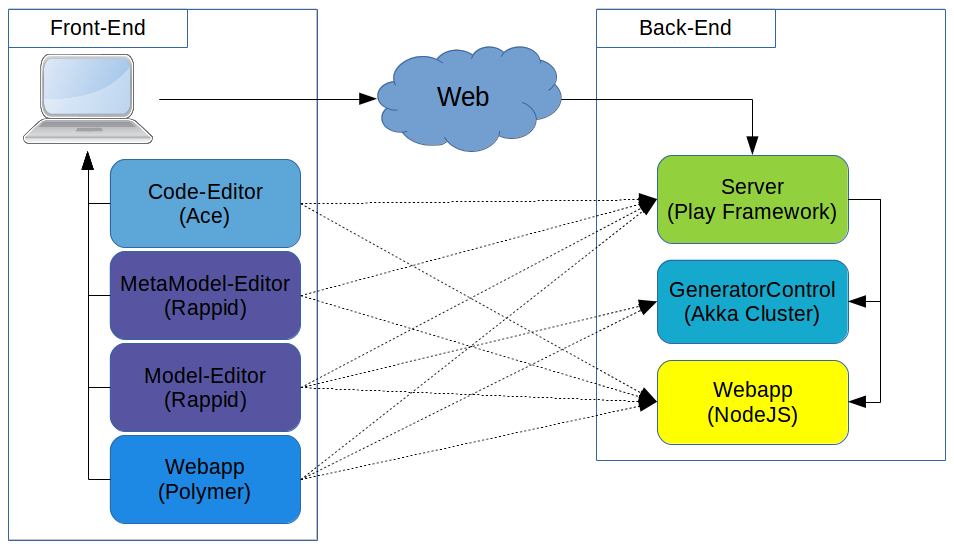
\includegraphics[width=5in]{figures/overview-final.png}
    \caption{Zielzustand - Übersicht}
    \label{fig:ZETA_OVERVIEW_NEW}
\end{figure}

Der Code-Editor ist zur Bearbeitung der Definition über die textuellen \acp{dsl} Style, Shape und Diagram zuständig. Dabei baut der Code-Editor von \textit{Zeta} wie zuvor auf den webbasierten Code Editor \ac{ace} auf. Die Konfiguration und Initialisierung wurde zudem im Rahmen dieser Arbeit und in Zusammenarbeit mit Patrick Leber von \textit{ScalaJS} auf JavaScript portiert und die Hauptdatei ist \textit{webapp/src/code-editor.js} \cite{zeta_code_editor,zeta_commit_code_editor}. Aus diesem Grund ist die gesamte \textit{ScalaJS} Umgebung überflüssig geworden und im Scala Projekt konnten die Unterprojekte \textit{Client} und \textit{Shared} entfernt werden \cite{zeta_commit_remove_sbt_client,zeta_commit_remove_sbt_shared}. Eine direkte Nutzung des \ac{ace} Editor ist nicht möglich, da das JavaScript Module System von \ac{ace} nicht mit \textit{Webpack} kompatibel ist. Aus diesem Grund wird bei \textit{Zeta} der Umweg über die Browserify kompatible und somit auch \textit{Webpack} kompatible Variante namens \textit{brace} gegangen. Bei der Portierung zu JavaScript sind zudem erstmal die Kollaboration und Autospeichern Funktion des Code-Editors entfernt worden, da der gewählte Ansatz unter anderem auf der Datenbank eine erhöhte Last verursacht hat und eine zukünftige Lösung ohne Persistierung arbeiten soll.

Die graphischen Editoren umfassen den Concept- und den Model-Editor. Beide Editoren basieren auf dem properitären \textit{Rappid} Editor. Der ehemalige MetaModel-Editor wurde aufgrund einer Umbenennung der grundlegenden Datenstruktur zum Concept-Editor umbenannt. Die Konfiguration für den Concept-Editor ist statisch definiert und die ist im Rahmen dieser Arbeit vom \textit{Play Server} zu \textit{Webpack} migriert worden \cite{zeta_commit_resolve_via_webpack}. Eintrittspunkt für den Concept-Editor ist die \textit{webapp/src/graphical-meta-model-editor.js} Datei und von hier aus werden die für den Concept-Editor relevanten Dateien über das \ac{es6} Module System geladen. Der Model-Editor ist auch im Rahmen dieser Arbeit in weiten Teilen zu \textit{Webpack} migriert worden. Die Konfiguration ist aber anders als beim Concept-Editor spezifisch für jedes Projekt und muss deswegen dynamisch erzeugt werden. Aktuell basiert das Ganze noch darauf, dass die Definitionen der textuellen \acp{dsl} aus dem Code-Editor mit den Definitionen aus dem Concept-Editor über einen Parser namens \textit{SprayParser} in ein Model unter \textit{de.htwg.zeta.server.generator.model} überführt wird. Auf Basis dieses Models werden über Generatoren im \textit{Play Server} JavaScript-Dateien erzeugt und in der Datenbank persistiert. Beim Aufruf des Model-Editors im Browser werden diese JavaScript Dateien zur Konfiguration des \textit{Rappid} Editors neben der JavaScript Datei von \textit{Webpack} geladen. Langfristig soll dieser proprietäre Ansatz durch Daten aus der \ac{rest} \ac{api} ersetzt werden. Anhand der Daten aus der \ac{rest} \ac{api} wird im Browser dann die spezifische Konfiguration für den \textit{Rappid} Editor erzeugt. Im Rahmen dieser Arbeit und in Zusammenarbeit mit Jan Bodendorf wurde die Generierung der Konfiguration auf Basis der \ac{rest} \ac{api} implementiert, aber noch nicht in den Model-Editor eingebunden \cite{zeta_milestone_2}. Eine Dokumentation über das Schema der \ac{rest} \ac{api} für die Erzeugung der Konfiguration des Model-Editors existiert auch, aber die Implementierung wurde innerhalb des aktuellen Teamprojekts zeitlich nach hinter verlagert \cite{zeta_wiki_rest_api}.

Die Webapp ist eine \ac{spa} und basiert auf der \textit{Polymer} Bibliothek. Die Implementierung der Webapp befindet sich im Verzeichnis \textit{webapp/src/app/} und bietet die Oberfläche zur Verwaltung der Generatoren. Dies umfasst das Erstellen, Löschen und Ausführen von Generatoren. Des Weiteren können die Transformationsregeln für die Generatoren definiert werden. Zusätzlich können noch in Scala geschriebene Filter für das genutzte Meta Modell eines Generators definiert werden. Aufbauend auf den Generatoren können noch verschiedenartige Task wie z.B. ein \textit{Timed Task} definiert werden. Im Gegensatz zum Ausgangszustand ist die Webapp nicht mehr direkt an eine Datenbank angebunden, sondern nutzt zum Großteil eigens für die Webapp erstellte \ac{rest} \ac{api} Endpoints. Um dies zu ermöglichen wurde im Rahmen dieser Arbeit die Implementierung zur Interaktion mit dem Backend gänzlich ausgetauscht \cite{zeta_commit_webapp_persist}.

\section{Back-End}

Bei der Beschreibung des Backends wird auf eine die verschiedenen Teilbereiche und ihre Dienste eingegangen. Zunächst wird die auf Laufzeitumgebung per \textit{Docker Compose} eingegangen. Danach folgt die Aufteilung der primär in Scala geschriebenen Implementierung von \textit{Zeta} für das Back-End und der neu eingeführten Qualitätssicherung per statische Code Analyse und der Testabdeckung per Unittests. Als nächstes wird auf die Teilkomponenten des \textit{Play Server} eingegangen, wie den Webservices und Websocket \acp{api}. Abschließend wird \textit{Akka Cluster} zur Verwaltung der Generatoren und die Ausführung der Generatoren über eigene \textit{Docker Container} beschrieben.

\subsection{Docker Compose}

Die Laufzeitumgebung ist für \textit{Zeta} weiterhin per \textit{Docker Compose} definiert und ist im Vergleich zur Ausgangsarchitektur im Rahmen dieser Arbeit in wesentlichen Bereichen vereinfacht worden. Der \textit{Play Server} nimmt nun, wie in Abbildung~\ref{fig:ZETA_ARCH_NEW} auf Seite~\pageref{fig:ZETA_ARCH_NEW} zu sehen, sämtliche externen Anfragen stellvertretend für alle Dienst an und leitet diese gegebenenfalls an den \textit{GeneratorControl} oder den \textit{Webapp} Dienst weiter. Die meisten der Anfragen werden jedoch schon innerhalb des \textit{Play Servers} verarbeitet, da der \textit{Play Server} z.B. für sämtliche \ac{rest} \acp{api} zuständig ist. Für den \textit{Akka Cluster} wird nun minimal nur noch ein einziger Dienst benötigt. Dies wird durch die Trennung der Startparameter ermöglicht und somit kann jeweils der \textit{Master}, der \textit{Developer} oder der \textit{Worker} konfiguriert werden. Der \textit{GeneratorControl} benötigt weiterhin Zugriff auf die \textit{Docker} \ac{api} um die Generatoren über externe \textit{Docker Container} auszuführen. Die Generatoren benötigen weiterhin Zugriff auf die \textit{Mongodb} zur Persistierung und auf den \textit{Play Server} zum Starten von weiteren Generatoren. Inzwischen wird nur noch die eine MongoDB als zentrale Datenbank genutzt und der Zugriff ist nur innerhalb des Backend möglich.

\begin{figure}
    \centering
    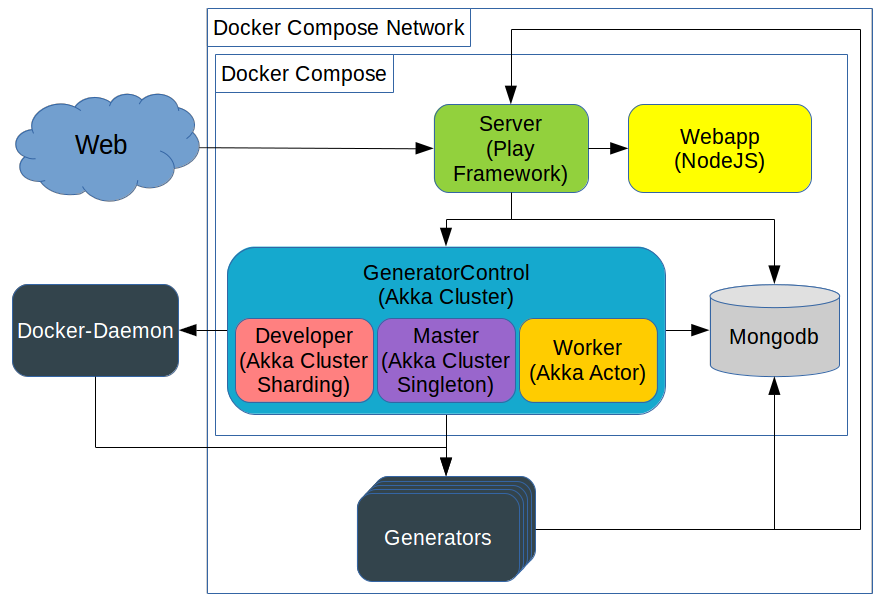
\includegraphics[width=5in]{figures/docker-compose-final.png}
    \caption{Zielzustand - Dienste}
    \label{fig:ZETA_ARCH_NEW}
\end{figure}

Zum Starten von \textit{Zeta} ist nun nur noch der Befehl \textit{docker-compose up} notwendig. Dies ist möglich indem nun für die Dienste nicht mehr über das Build Tool \ac{sbt} zuvor \textit{Docker Images} erzeugt werden müssen, sondern die Dienste wie der \textit{Play Server} und \textit{generatorControl} werden nun direkt über \ac{sbt} ausgeführt. Der Vorteil besteht darin, dass nun die verschiedensten \ac{sbt} Plugins für Entwicklersysteme genutzt werden können. Zuvor liefen die Dienste ohne \ac{sbt} und wurden direkt über gepackte JARs ausgeführt. Zum jetzigen Zeitpunkt wird aber kein offizielles \textit{Docker Image} für \ac{sbt} angeboten und die \textit{Docker Images} aus der Community sind entweder veraltet, bieten keine Auswahl einer spezifischen Java Version an oder haben nur eine Variante der offiziellen Java Images. Aus diesem Grund wurde ein eigenes \textit{Docker Image} für \ac{sbt} definiert und die genaue Definition kann im Programmcode~\ref{lst:ZETA_DOCKERFILE_SBT} auf Seite~\pageref{lst:ZETA_DOCKERFILE_SBT} nachvollzogen werden. Zuvor basierten die erzeugten \textit{Docker Images} für die Dienste auf \textit{openjdk:latest} mit einer unkomprimierten Gesamtgröße von 738 MB. Das eigene \textit{Docker Image} für \ac{sbt} basiert jedoch auf \textit{openjdk:8u151-jdk-alpine3.7} und ist mit einer unkomprimierten Gesamtgröße von 102 MB nur etwa 14\% der Größe des zuvor genutzten Images. Mit der Nutzung eines spezifischen \textit{Docker Image} ist nun auch die genutzte Java Version schon über den Namen des Image nachvollziehbar und die Kompatibilität zwischen den Entwicklersystem wird gewährleistet. Allgemein wurde nun bei allen Diensten auf die Nutzung eines spezifischen Images anstelle eines Bereichs verschiedener Versionen eines Images umgestellt.

\bigskip
\lstinputlisting[language=dockerfile, breaklines=true, caption={[SBT Dockerfile] SBT Dockerfile \cite{zeta_new_dockerfile}},label={lst:ZETA_DOCKERFILE_SBT}]{listings/Dockerfile.new}
\smallskip

Das \ac{sbt} Image wird nun wie im Programmcode~\ref{lst:ZETA_COMPOSE_GENERATOR} auf Seite~\pageref{lst:ZETA_COMPOSE_GENERATOR} genutzt um z.B. den \textit{generatorControl} Dienst zu definieren. Dabei ist zu sehen, dass das gesamte Scala Projekte aus dem Verzeichnis \textit{api} in den \textit{Docker Container} gemapped wird. Damit ist es nun möglich z.B. bei einen Neustart des Dienstes Änderungen zu kompilieren. Zusätzlich wird jeweils ein eigenes Verzeichnis für die \ac{sbt} Dateien wie dem Cache in das \textit{root} Verzeichnis gemapped. Des Weiteren werden die \textit{Docker} spezifischen Einstellungen nun über Umgebungsvariablen an den \textit{Docker Container} übergeben. Diese Erweiterung ist auch beim Dienst für den \textit{Play Server} durchgeführt worden. 

\bigskip
\lstinputlisting[language=docker-compose, breaklines=true, caption={[GeneratorControl Dienst - docker-compose.yml] GeneratorControl Dienst - docker-compose.yml \cite{zeta_new_docker_compose}},label={lst:ZETA_COMPOSE_GENERATOR}, firstline=3, lastline=14]{listings/docker-compose.new.yml}
\smallskip

Der \textit{webapp} Dienst basiert nun, wie in Programmcode~\ref{lst:ZETA_COMPOSE_WEBAPP} auf Seite~\pageref{lst:ZETA_COMPOSE_WEBAPP} zu sehen,  direkt auf dem offiziellen Image für \textit{Node.js} und nicht mehr wie zuvor auf einem eigens definierten Image \cite{zeta_webapp_image}. Ein Wechsel auf die minimale Alpine Variante ist nicht möglich gewesen, da dieser einige Abhängigkeiten wie z.B. die \textit{ace-grammer} Bibliothek nicht auf \ac{npm} zur Verfügung stehen und muss deshalb direkt von Github bezogen werden \cite{zeta_new_package_json}. Die Entscheidung zu Gunsten der um ein vielfaches größeren Standard Variante des \textit{Node.js} Image gegenüber eines eigenen Images mit Git auf Basis der Alpine Variante ist aufgrund der einfacheren Konfiguration des \textit{webapp} Dienstes gefallen. Ein eigens für die Webapp definiertes \textit{Docker Image} erhöht die Komplexität der \textit{Docker Compose} Konfiguration. Des Weiteren wird für den \textit{webapp} Dienst \textit{Yarn} als alternativer \ac{npm} Package Manager für eine schnellere Auflösung der Abhängigkeiten genutzt. Die Nutzung von \textit{Bower} als weiteren Package Manager ist nun direkt in den Installationsprozess der Abhängigkeiten von \textit{Yarn} integriert.

\bigskip
\lstinputlisting[language=docker-compose, breaklines=true, caption={[Webapp Dienst - docker-compose.yml] Webapp Dienst - docker-compose.yml \cite{zeta_new_docker_compose}},label={lst:ZETA_COMPOSE_WEBAPP}, firstline=42, lastline=47]{listings/docker-compose.new.yml}
\smallskip

Zur Laufzeit von \textit{Zeta} werden weiterhin mehrere \textit{Docker Images} zur Ausführung der Generatoren mit den Transformationsregeln benötigt. Diese Images können aber nun über den in \textit{Docker Compose} definierten \textit{images} Dienst erzeugt werden. Der Dienst kann per \textit{docker-compose up images} gestartet werden und beendet sich automatisch nach der Erzeugung der \textit{Docker Images}. Somit wird für den Betrieb von \textit{Zeta} nur noch \textit{Docker} mit \textit{Docker Compose} benötigt. Java oder auch \ac{sbt} muss auf dem Hostsystem nicht installiert werden, da dies über \textit{Docker Composer} abgefangen wird.  

\subsection{Scala Projekt}

Im Backend werden mehrere eigens für \textit{Zeta} entwickelte Dienste verwendet. Diese Dienste umfassen den \textit{Play Server}, den \textit{generatorControl} und die Generatoren. Dabei sind alle diese Dienste mit Scala implementiert und sind in einem gemeinsamen Scala Projekte im Verzeichnis \textit{api} zusammengefasst. Als Build Tool wird hierbei auf \ac{sbt} gesetzt. \textit{Zeta} nutzt einige Plugins für \ac{sbt} um z.B. eine Qualitätssicherung über Linter zu ermöglichen oder die verschiedenen Abhängigkeiten der Unterprojekte zu visualisieren. Eine Übersicht kann in der Tabelle~\ref{tab:ZETA_SBT_NEW} auf Seite~\pageref{tab:ZETA_SBT_NEW} gefunden werden. Im Gegensatz zur Ausgangsarchitektur aus dem Unterabschnitt~\ref{sec:INITIAL_BUILD} ab Seite~\pageref{sec:INITIAL_BUILD} wurden alle \ac{sbt} Plugins für \textit{SbtWeb} entfernt, da diese nicht länger benötigt werden.

\begin{table}[ht]
    \smallskip
    \centering
    \begin{tabular}{| l | l | l |}
    \hline
    \bf GroupID & \bf ArtifactID & \bf Beschreibung \\ \hline
    com.timushev.sbt & sbt-updates & Prüft auf neuere Versionen \\ \hline
    com.typesafe.play & sbt-plugin & Play Framework Dev Features \\ \hline
    com.typesafe.sbt & sbt-native-packager & Generiert Docker Images \\ \hline
    net.virtual-void & sbt-dependency-graph & Visualisiert Abhängigkeiten \\ \hline
    org.scalastyle & scalastyle-sbt-plugin & Scala Linter\\ \hline
    org.wartremover & sbt-wartremover & Scala Linter \\ \hline
    \end{tabular}
    \caption{Zielzustand - sbt Plugins \cite{zeta_new_sbt_plugins}}
    \label{tab:ZETA_SBT_NEW}
\end{table}

Die Implementierung innerhalb des \ac{sbt} Projekts ist in mehrere Unterprojekte aufgeteilt. Eine Übersicht der verschiedene Unterprojekte kann in Abbildung~\ref{fig:ZETA_SBT_NEW} auf Seite~\pageref{fig:ZETA_SBT_NEW} eingesehen werden. Dabei sind die genutzten Package Präfixe bei den verschiedenen Unterprojekten mit angegeben und enthalten untereinander keine zyklischen Abhängigkeiten. Der Umfang der verschiedenen Unterprojekte kann in der Tabelle~\ref{tab:ZETA_METRICS_LOC_NEW} auf Seite~\pageref{tab:ZETA_METRICS_LOC_NEW} eingesehen werden. Anders als z.B. ein Maven Projekt mit mehreren Modulen hat ein \ac{sbt} Projekt mit mehreren Unterprojekten nur eine gemeinsame Konfiguration für alle Unterprojekte. Von Nicolas Wehrle wurde jedoch die zentrale \textit{build.sbt} in eine \textit{built.sbt} pro Unterprojekt aufgeteilt.

Das \textit{Common} Projekt ist eines der zentralen Unterprojekte von dem alle anderen Unterprojekte abhängig sind und enthält unter anderem die Klassen für die Datenbank Entities. Aber auch einige hilfreiche Klassen für die \textit{Akka Actoren} und die Formatter für die Transformationen innerhalb der \ac{rest} \ac{api} und MongoDb Persistierung von \ac{json} zu einem Objekt und zurück. Auf dem \textit{Common} Unterprojekt baut wiederum mit dem \textit{Persistence} Projekt das zweite zentrale Unterprojekt auf. Das \textit{Persistence} Unterprojekt ist unter Patrick Leber neu zu \textit{Zeta} hinzugefügt worden und enthält die Implementierung für die Interaktion mit der MongoDB. Das umfasst die gängigen Aktionen wie z.B. Auslesen, Modifizieren, Löschen und Erstellen von Einträgen in der Datenbank. Die genutzte Implementierung für MongoDB wird über ein Module des \ac{di} Frameworks Guice konfiguriert und ersetzt die zuvor vorhandene Implementierung für Persistierung \cite{zeta_new_persistence_module}.

\begin{figure}
    \centering
    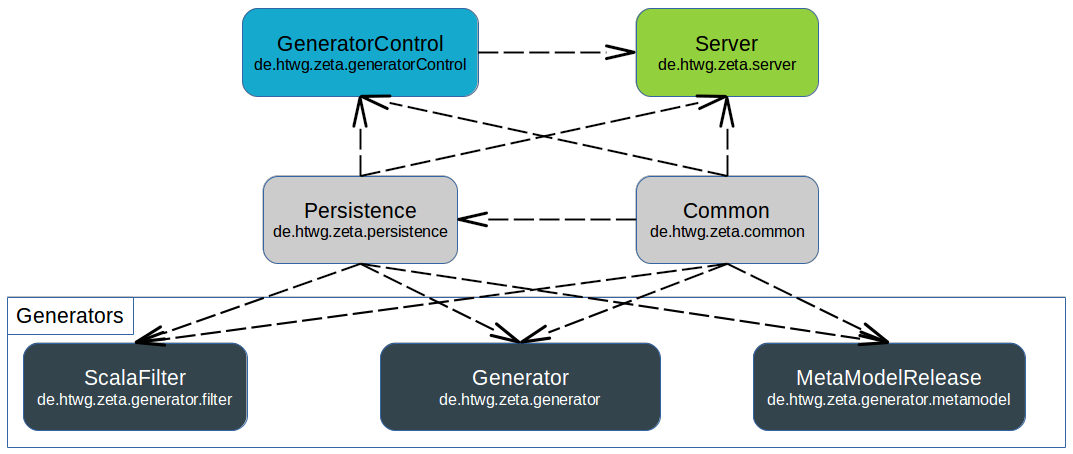
\includegraphics[width=5in]{figures/sbt-modules-final.png}
    \caption{Zielzustand - Abhängigkeiten der \ac{sbt} Unterprojekte}
    \label{fig:ZETA_SBT_NEW}
\end{figure}

\begin{table}[ht]
    \smallskip
    \centering
    \begin{tabular}{| l | r | r | r |}
    \hline
    \bf Projekt & \bf Gesamt & \bf SLOC & \bf CLOC \\ \hline
    common & 3937 (+570) & 2868 (+710) & 363 (-335) \\ \hline
    generatorControl & 2828 (+571) & 2183 (+471) & 167 (-28) \\ \hline
    scalaFilter & 144 (+19) & 119 (+105) & 3 (+3) \\ \hline
    generator & 528 (+528) & 377 (+377) & 92 (+92) \\ \hline
    metaModelRelease & 76 (+11) & 57 (+5) & 7 (+7) \\ \hline
    persistence & 3153 (+3153) & 2123 (+2123) & 520 (+520) \\ \hline
    server & 13657 (+3117) & 9650 (+2273) & 1731 (-107) \\ \hline
    \bf Gesamt & \bf 24323 (+5634) & \bf 17377 (+4118) & \bf 2883 (-83) \\ \hline
    \end{tabular}
    \caption{Zielzustand - \ac{loc} der Scala Dateien \cite{analys_new_directory}}
    \label{tab:ZETA_METRICS_LOC_NEW}
\end{table}

Der \textit{Play Server} befindet sich im \textit{Server} Unterprojekt und ist die öffentliche \ac{api} von \textit{Zeta}. Der \textit{Play Server} ist auf Basis des \textit{Play Frameworks} implementiert und hat nicht die Standard Maven Ordnerstruktur \cite{play_framework_anatomy}. Die Implementierung befindet sich im \textit{app} Verzeichnis, die Konfigurationsdateien wie z.B. die \textit{application.conf} oder \textit{routes} sind im \textit{conf} Verzeichnis und die Tests sind im \textit{test} Verzeichnis. Mit der Einführung von Package Präfixen unter Nicolas Wehrle sind die meisten Klassen des \textit{Play Server} in das Verzeichnis \textit{app/de/htwg/zeta/server} gewandert und entspricht somit nicht mehr der Standard Verzeichnisstruktur des \textit{Play Frameworks}. Der Aufbau des \textit{de.htwg.zeta.server} Paket kann in der Tabelle~\ref{tab:ZETA_NEW_PLAY_PACKAGES} auf Seite~\pageref{tab:ZETA_NEW_PLAY_PACKAGES} betrachtet werden. Im \text{app} Verzeichnis sind zusätzlich noch die Ordner \textit{controllers} mit der Konfiguration, ob eine Route nur für angemeldete Benutzer verfügbar ist, und das \textit{views} Verzeichnis mit den \ac{html} Templates. 

\begin{table}[ht]
    \smallskip
    \centering
    \begin{tabular}{| l | r | r | r | r | r |}
    \hline
    \bf Projekt & \bf Dateien & \bf Ordner & \bf Klassen & \bf Methoden & \bf Traits \\ \hline
    common & 65 (+29) & 13 (-3) & 167 (+0) & 194 (-33) & 28 (+12) \\ \hline
    generatorControl & 33 (+6) & 10 (+2) & 117 (+12) & 191 (+40) & 12 (-23) \\ \hline
    scalaFilter & 2 (+0) & 1 (-1) & 2 (+0) & 6 (+1) & 1 (+0) \\ \hline
    generator & 5 (+5) & 1 (+1) & 13 (+13) & 24 (+24) & 0 (+0) \\ \hline
    metaModelRelease & 1 (+0) & 1 (+0) & 2 (+0) & 0 (-1) & 0 (+0) \\ \hline
    persistence & 30 (+30) & 7 (+7) & 109 (+109) & 189 (+189) & 19 (+19) \\ \hline
    server & 232 (+78) & 49 (+2) & 407 (+138) & 1115 (+357) & 42 (+12)  \\ \hline
    \bf Gesamt & \bf 368 (+121) & \bf 82 (-3) & \bf 817 (+185) & \bf 1719 (+9) & \bf 102 (+6) \\ \hline
    \end{tabular}
    \caption{Zielzustand - Metriken über Scala Typen \cite{analys_new_directory}}
    \label{tab:ZETA_METRICS_NEW}
\end{table}

Das \textit{GeneratorControl} Unterprojekte basiert auf einem \textit{Akka Cluster} und ist für die Verwaltung der Generatoren zuständig \cite{akka_cluster}. Dabei werden die Anfragen von der Webapp aus dem Frontend verarbeitet und ein entsprechender Generator mit den Transformationsregeln über einen neuen \textit{Docker Container} ausgeführt. Die Generatoren umfassen die Unterprojekte \textit{ScalaFilter}, \textit{Generator} und \textit{MetaModelRelease}. Im Rahmen dieser Arbeit wurden die Unterprojekte \textit{BasicGenerator}, \textit{FileGenerator}, \textit{SpecificGenerator}, \textit{RemoteGenerator} und \textit{Template} aus der Abbildung~\ref{fig:ZETA_SBT_OLD} auf Seite~\pageref{fig:ZETA_SBT_OLD} zu dem Unterprojekte \textit{Generator} zusammengefasst. Diese Änderung wurde aufgrund der Bewertung der Generatoren aus dem Unterabschnitt~\ref{subsec:REVIEW_MODULES} ab Seite~\pageref{subsec:REVIEW_MODULES} durchgeführt und soll eine zu starke Modularisierung der Unterprojekte beheben.

\begin{table}[ht]
    \smallskip
    \centering
    \begin{tabular}{| l | l |}
    \hline
    \bf Paket & \bf Beschreibung \\ \hline
    actor & Akka Actoren \\ \hline
    controllers & Siehe \ac{mvc} Entwurfsmuster \\ \hline
    forms & Play Formular Definitionen \\ \hline
    generator & SprayParser und Models mit JavaScript Generatoren \\ \hline
    model & Meta Modell Actoren und Validator  \\ \hline
    module & Google Guice \ac{di} Module  \\ \hline
    routing & Mapper für Route auf Controller\\ \hline
    silhouette & Silhoutte Abhängige Authentifizierung \\ \hline
    start & Play Framework Bootstrap \\ \hline
    util & Allgemeine Hilfsklassen \\ \hline
    \end{tabular}
    \caption{Ausgangszustand - Play Server Pakete (de.htwg.zeta.server)}
    \label{tab:ZETA_NEW_PLAY_PACKAGES}
\end{table}

\subsection{Linter und Testabdeckung}

\textit{Zeta} verwendet in seinem Ausgangszustand nur die Linter des Scala Compilers zur längerfristigen Qualitätssicherung und die vorhandenen Unittests sind in einem nicht verwendbaren Zustand. Eine tiefere Beschreibung der Gesamtsituation kann im Unterabschnitt~\ref{subsec:REVIEW_QA} ab Seite~\pageref{subsec:REVIEW_QA} eingesehen werden. Wie in der Tabelle~\ref{tab:ZETA_SBT_NEW} auf Seite~\pageref{tab:ZETA_SBT_NEW} zusehen, verwendet \textit{Zeta} nun zusätzliche Linter. Die beiden Linter \textit{Wartremover} und \textit{Scalastyle} sind im Rahmen dieser Arbeit bei \textit{Zeta} ergänzt worden \cite{zeta_commit_linter,wartremover,scalastyle}. Der \textit{Wartremover} ist ein Plugin für den Scala Compiler und führt die Prüfungen beim Kompilieren der geänderten Scala Dateien aus. Die Konfiguration des \textit{Wartremover} für \textit{Zeta} meldet alle Probleme als Warnugen und bis auf den \textit{NonUnitStatements} sind alle Prüfungen aktiviert. \textit{Scalastyle} wiederrum kann z.B. über den \textit{scalastyle} Task per \ac{sbt} ausgeführt werden und ist zusätzlich an den \textit{Compile} Task von \ac{sbt} angehängt um ähnlich wie der \textit{Wartremover} beim Kompilierungsvorgang ausgeführt zu werden \cite{zeta_new_build}. Für \textit{Scalastyle} wird eine auf \textit{Zeta} angepasste Konfiguration verwendet und viele der gemeldeten Probleme wie z.B. vom \textit{UnderscoreImportChecker} sind im Rahmen dieser Arbeit behoben worden \cite{zeta_new_scalastyle,zeta_commit_UnderscoreImport}. Eine Übersicht der aktuell gemeldeten Probleme im Vergleich zum Ausgangszustand pro Unterprojekt befindet sich in der Tabelle~\ref{tab:ZETA_METRICS_LINT_NEW} auf Seite~\pageref{tab:ZETA_METRICS_LINT_NEW}.

\begin{table}[ht]
    \smallskip
    \centering
    \begin{tabular}{| l | r | r |}
    \hline
    \bf Projekt & \bf Compile with & \bf Scalastyle \\ 
    ~ & \bf Wartremover & (Err./War.) \\ 
    ~ & (Err./War.) & ~ \\ \hline
    common & 0 / 37 (0 / -50) & 0 / 82 (-67 / -151) \\ \hline
    generatorControl & 0 / 77 (+0 / -2) & 0 / 109 (-69 / -130) \\ \hline
    scalaFilter & 0 / 1 (+0 / -10) & 0 / 1 (-2 / -7) \\ \hline
    generator & 0 / 2 (+0 / +2) & 0 / 2 (+0 / +2) \\ \hline
    metaModelRelease & 0 / 0 (+0 / -2) & 0 / 0 (-1 / -4) \\ \hline
    persistence & 0 / 33 (+0 / +33) & 0 / 19 (+0 / +19) \\ \hline
    server & 0 / 563 (+0 / -267) & 0 / 922 (-264 / -1822) \\ \hline
    \bf Gesamt & \bf 0 / 713 (+0 / -411) & \bf 0 / 1135 (-437 / -2375) \\ \hline
    \end{tabular}
    \caption{Zielzustand - Ergebnisse der Linter Prüfungen \cite[Scalastyle]{analys_new}}
    \label{tab:ZETA_METRICS_LINT_NEW}
\end{table}

Für die Unittests wird einheitlich für alle Unterprojekt das Unittest Framework \textit{ScalaTest} verwendet und zur Prüfung der Testabdeckung wird zusätzlich \textit{scoverage} verwendet \cite{scalatest_project,scoverage}. Der aktuelle Stand der Unittests hat sich im Vergleich zum Ausgangszustand aus dem Unterabschnitt~\ref{subsec:REVIEW_QA} ab Seite~\pageref{subsec:REVIEW_QA} deutlich verändert. Der aktuelle Stand der Unittests und ihre Testabdeckung pro Unterprojekte befindet sich in der Tabelle~\ref{tab:ZETA_METRICS_TESTS_NEW} auf Seite~\pageref{tab:ZETA_METRICS_TESTS_NEW}. Sind im Ausgangszustand nur ingesamt drei Unittests vorhanden gewesenen, sind es nun über 800 verschiedene Unittests. Im Ausgangszustand konnte keiner der Unittests ausgeführt werden und nun können alle Unittests ausgeführt werden. Aktuell schlagen mit rund 3 \% aller Unittests einige der Unittests im \textit{Play Server} fehl. Die ermittelte Testabdeckung für Statements und Verzweigungen im Programmcode über alle Scala Dateien befindet sich nun im niedrigen zweistelligen Prozentbereich und ist im Vergleich zum Ausgangszustand ein ausreichender Zustand. Von einer minimalen Testabdeckung von z.B. 70 - 80 \% ist dies aber noch weit entfernt.

\begin{table}[ht]
    \smallskip
    \centering
    \begin{tabular}{| l | r | r | r | r |}
    \hline
    \bf Projekt & \bf Erfolgreich & \bf Fehlgeschlagen & \bf Statement & \bf Branch \\ \hline
    common & 1 & 0 & 5,57 \% & 0,00 \% \\ \hline
    generatorControl & 0 & 0 & 0,00 \% & 0,00 \% \\ \hline
    scalaFilter & 0 & 0 & 0,00 \% & 0,00 \% \\ \hline
    generator & 0 & 0 & 0,00 \% & 0,00 \% \\ \hline
    metaModelRelease & 0 & 0 & 0,00 \% & 0,00 \% \\ \hline
    persistence & 666 & 0 & 77,74 \% & 63,89 \% \\ \hline
    server & 134 & 21 & 10,03 \% & 16,54 \% \\ \hline
    \bf Gesamt & \bf 801 & \bf 21 & \bf 13,41 \% & \bf 16,24 \% \\ \hline
    \end{tabular}
    \caption{Zielzustand - Metriken über Unittests und Testabdeckung \cite[Scoverage]{analys_new_coverage,analys_new}}
    \label{tab:ZETA_METRICS_TESTS_NEW}
\end{table}

\subsection{Web \acp{api}}

Der \textit{Play Server} ist die öffentliche \ac{api} von \textit{Zeta} und stellt aus diesem Grund eine Reihe von Websockets und \ac{rest} Endpoints zur Verfügung. Eine Übersicht der verschiedenen Websockets kann in der Abbildung~\ref{fig:ZETA_WS_NEW} auf Seite~\pageref{fig:ZETA_WS_NEW} gefunden werden. Dabei ist der \textit{MetaModelWsActor} zusammen mit dem \textit{MetaModelWsMediatorActor} für den Abgleich zwischen mehreren Concept-Editor Instanzen für ein und dasselbe Projekt verantwortlich.

\begin{figure}
    \centering
    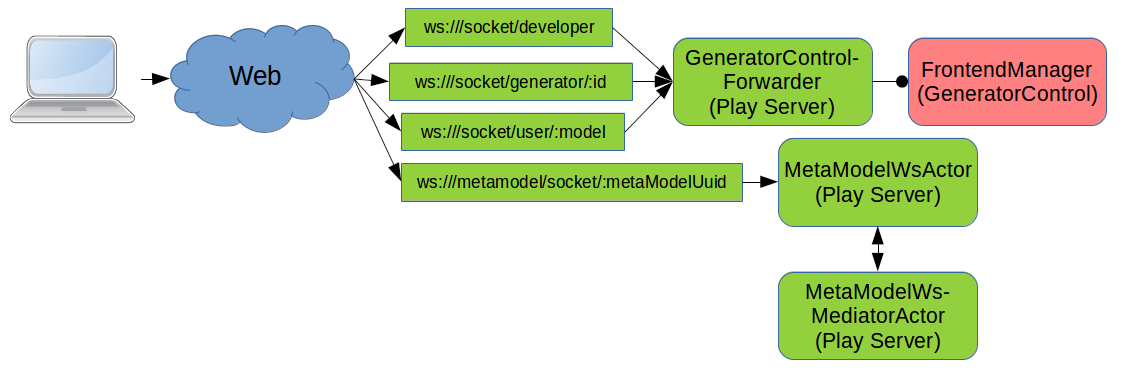
\includegraphics[width=5in]{figures/actor_play_final.png}
    \caption{Zielzustand - Websockets}
    \label{fig:ZETA_WS_NEW}
\end{figure}

Der \textit{Play Server} ist nun nicht mehr Teil des \textit{Akka Clusters} des {generatorControl} Dienst, sondern ist extern über einen Cluster Client an den \textit{generatorControl} Dienst angebunden. Die Anfragen von z.B. der Webapp werden über den \textit{GeneratorControlForwarder} Actor im \textit{Play Server} an den \textit{FrontendManager} Actor im \textit{generatorControl} Dienst \cite{akka_cluster_client} gesendet. Der \textit{FrontendManager} Actor gehört zur \textit{Developer} Node und sendet die Anfrage an den entsprechenden Actor innerhalb des \textit{Akka Clusters}.

\begin{table}[ht]
    \smallskip
    \centering
    \begin{tabular}{| l | l |}
    \hline
    \bf Method & \bf Route \\ \hline
    \colorbox{LimeGreen}{GET},\colorbox{LimeGreen}{POST} & /rest/v1/meta-models \\ \hline
    \colorbox{LimeGreen}{GET},\colorbox{red}{PUT} & /rest/v1/meta-models/:id \\ \hline
    \colorbox{LimeGreen}{DELETE} & /rest/v1/meta-models/:id \\ \hline
    \colorbox{red}{GET},\colorbox{LimeGreen}{PUT} & /rest/v1/meta-models/:id/definition \\ \hline
    \colorbox{red}{GET} & /rest/v1/meta-models/:id/definition/mclasses \\ \hline
    \colorbox{red}{GET} & /rest/v1/meta-models/:id/definition/mreferences \\ \hline
    \colorbox{red}{GET} & /rest/v1/meta-models/:id/definition/mclasses/:name \\ \hline
    \colorbox{red}{GET} & /rest/v1/meta-models/:id/definition/mreferences/:name \\ \hline
    \colorbox{red}{GET},\colorbox{LimeGreen}{PUT} & /rest/v1/meta-models/:id/shape \\ \hline
    \colorbox{red}{GET},\colorbox{LimeGreen}{PUT} & /rest/v1/meta-models/:id/style \\ \hline
    \colorbox{red}{GET},\colorbox{LimeGreen}{PUT} & /rest/v1/meta-models/:id/diagram \\ \hline
    \colorbox{LimeGreen}{GET} & /rest/v1/meta-models/:id/validator \\ \hline
    \colorbox{red}{PUT} & /rest/vl/meta-models/:id/classMethod/:method/:class \\ \hline
    \colorbox{red}{PUT} & /rest/vl/meta-models/:id/referenceMethod/:method/:ref \\ \hline
    \colorbox{red}{GET} & /rest/vl/meta-models/:id/commonMethod/:method \\ \hline
    \end{tabular}
    \caption{Zielzustand - Rest Endpoints MetaModel}
    \label{tab:ZETA_REST_META_NEW}
\end{table}

Auf Seiten der \ac{rest} \ac{api} Endpoints hat sich strukturell einiges verändert. Im Rahmen dieser Arbeit wurde der Prefix \textit{/rest/v1} zu allen \ac{rest} Endpoints hinzugefügt. Dies soll eine einfachere Unterscheidung zwischen einer Route zu einem \ac{html} Dokument und eines \ac{rest} Endpoints ermöglichen. Zusätzlich sollte durch das \textit{v1} eine Versionierung der \ac{rest} \ac{api} direkt erkennbar sein \cite{webservice_versioning}. Somit soll bei den Entwicklern für \textit{Zeta} ein stärkeres Bewusstsein für Breaking Changes hervorgerufen werden. Falls die Route eines \ac{rest} Endpoints geändert wird oder Umbenennungen im Schema stattfinden, kann dies zu Fehlern im Frontend führen. Eine Übersicht der \ac{rest} Endpoints für das Meta Modell und das Modell kann in der Tabelle~\ref{tab:ZETA_REST_META_NEW} auf Seite~\pageref{tab:ZETA_REST_META_NEW} und in der Tabelle~\ref{tab:ZETA_REST_MODEL_NEW} auf Seite~\pageref{tab:ZETA_REST_MODEL_NEW} gefunden werden. In den Tabellen ist die Hintergrundfarbe bei der \ac{http} Methode ein Indikator für die Nutzung des Endpoints. Grün als Hintergrundfarbe bedeutet, dass der Endpoint innerhalb von \textit{Zeta} im Frontend genutzt wird. Rot als Hintergrundfarbe wiederum zeigt, dass der Endpoint nirgends in \textit{Zeta} genutzt wird. In den Tabellen sind viele ungenutzte \ac{rest} Endpoints für die \ac{http} \textit{GET} Methode zusehen, die in der Route \textit{/:id/definition} enthalten. Diese Routen werden immer spezifischer und dabei werden die Rückgaben aus dem Endpoint immer weiter gefiltert. Diese spezifischeren Endpoints bieten im Vergleich zu den allgemeineren \ac{rest} Endpoints aber nicht detailliertere Informationen an. Der aktuelle Ansatz nutzt die allgemeinen \ac{rest} Endpoints wie z.B. \textit{/rest/v1/meta-models/:id} und filtert die Rückgabe im Browser entsprechend der gegebenen Anforderungen.   

\begin{table}[ht]
    \smallskip
    \centering
    \begin{tabular}{| l | l |}
    \hline
    \bf Method & \bf Route \\ \hline
    \colorbox{red}{GET},\colorbox{LimeGreen}{POST} & /rest/v1/models \\ \hline
    \colorbox{red}{GET},\colorbox{red}{PUT},\colorbox{LimeGreen}{DELETE} & /rest/v1/models/:id \\ \hline
    \colorbox{red}{GET},\colorbox{LimeGreen}{PUT} & /rest/v1/models/:id/definition \\ \hline
    \colorbox{red}{GET} & /rest/v1/models/:id/definition/nodes \\ \hline
    \colorbox{red}{GET} & /rest/v1/models/:id/definition/nodes/:name \\ \hline
    \colorbox{red}{GET} & /rest/v1/models/:id/definition/edges \\ \hline
    \colorbox{red}{GET} & /rest/v1/models/:id/definition/edges/:name \\ \hline
    \colorbox{LimeGreen}{GET} & /rest/v1/models/:id/validation \\ \hline
    \end{tabular}
    \caption{Zielzustand - Rest Endpoints Model}
    \label{tab:ZETA_REST_MODEL_NEW}
\end{table}

Neben den \ac{rest} Endpoints für das Meta Modell und Modell sind durch die Entfernung des Zugriffs auf die Datenbank im Frontend der Webapp einige neue Endpoints hinzugekommen. Eine List der neuen \ac{rest} Endpoints befindet sich in der Tabelle~\ref{tab:ZETA_REST_APP_OLD} auf Seite~\pageref{tab:ZETA_REST_APP_OLD}. Die Hintergrundfarbe ist derselbe Indikator wie bei den beiden vorherigen Tabellen über die \ac{rest} Endoints für das Meta Modell und Modell. 

\begin{table}[ht]
    \smallskip
    \centering
    \begin{tabular}{| l | l |}
    \hline
    \bf Method & \bf Route \\ \hline
    \colorbox{LimeGreen}{GET} & /rest/v1/generator-images \\ \hline
    \colorbox{LimeGreen}{GET} & /rest/v1/generators \\ \hline
    \colorbox{red}{GET},\colorbox{LimeGreen}{DELETE} & /rest/v1/generators/:id \\ \hline
    \colorbox{LimeGreen}{GET},\colorbox{LimeGreen}{POST} & /rest/v1/filters \\ \hline
    \colorbox{red}{GET},\colorbox{LimeGreen}{DELETE} & /rest/v1/filters/:id \\ \hline
    \colorbox{LimeGreen}{GET} & /rest/v1/meta-model-releases \\ \hline
    \colorbox{LimeGreen}{GET},\colorbox{LimeGreen}{POST} & /rest/v1/bonded-tasks \\ \hline
    \colorbox{LimeGreen}{DELETE} & /rest/v1/bonded-tasks/:id  \\ \hline
    \colorbox{LimeGreen}{GET},\colorbox{LimeGreen}{POST} & /rest/v1/event-driven-tasks \\ \hline
    \colorbox{LimeGreen}{DELETE} & /rest/v1/event-driven-tasks/:id \\ \hline
    \colorbox{LimeGreen}{GET},\colorbox{LimeGreen}{POST} & /rest/v1/timed-tasks \\ \hline
    \colorbox{LimeGreen}{DELETE} & /rest/v1/timed-tasks/:id \\ \hline
    \colorbox{LimeGreen}{GET},\colorbox{LimeGreen}{PUT} & /rest/v1/files/:id/*name \\ \hline
    \end{tabular}
    \caption{Zielzustand - Rest Endpoints Webapp}
    \label{tab:ZETA_REST_APP_OLD}
\end{table}

\subsection{Generator Verwaltung}

Die Verwaltung der Generatoren findet innerhalb des \textit{generatorControl} Dienstes statt und basiert auf einem \textit{Akka Cluster}. Dabei besteht der \textit{Akka Cluster} aus den drei Cluster Nodes \textit{Developer}, \textit{Master} und \textit{Worker}. Eine Übersicht der Kommunikationswege der Actoren des Akka Clusters befindet sich in der Abbildung~\ref{fig:ZETA_ACTOR_NEW} auf Seite~\pageref{fig:ZETA_ACTOR_NEW} und eine Übersicht der Hierachie der verschiedenen Actoren ist in Abbildung~\ref{fig:ZETA_HIERACHY_NEW} auf Seite~\pageref{fig:ZETA_HIERACHY_NEW}. Anfragen des \textit{Play Servers} werden vom \textit{FrontendManager} Actor als Teil der \textit{Developer} Node angenommen. Dabei wird bei den Anfragen zwischen einem \textit{DeveloperRequest}, \textit{GeneratorRequest} oder \textit{UserRequest} unterschieden. Innerhalb des \textit{Developer} Node findet die Kommunikation direkt über Actor Referenzen statt \cite{akka_actor}. Die Anfragen werden als nächstes vom \textit{Mediator} Actor an einen der entsprechenden Manager Actor weitergeleitet. Diese Manager Actoren wandeln die Anfrage in einen \textit{Job} Nachricht um und senden diesen weiterhin innerhalb der \textit{Developer} Node an den \textit{WorkQueue} Actor.

\begin{figure}
    \centering
    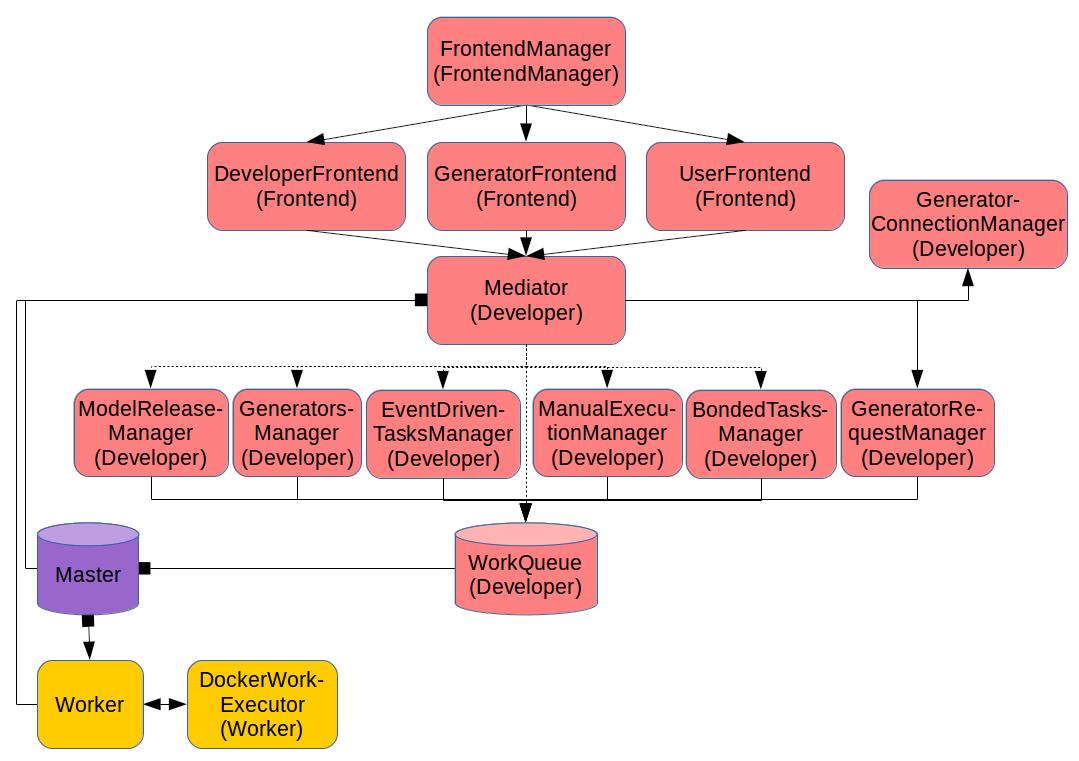
\includegraphics[width=5in]{figures/actor_backend_final.png}
    \caption{Zielzustand - Backend Actor System}
    \label{fig:ZETA_ACTOR_NEW}
\end{figure}

Der \textit{WorkQueue} Actor ist im Gegensatz zu den restlichen Actoren in der \textit{Developer} Node ein Persistent Actor mit einem internen Zustand der z.B. nach einem Absturz automatisch wiederhergestellt wird. Innerhalb des \textit{WorkQueue} Actor werden die \textit{Job} Nachrichten mit Zusatzinformation zu neuen Instanzen einer \textit{Work} Nachricht hinzugefügt und über den verteilten Publish Subscribe Mechanismus von Akka an den \textit{Master} Actoren der \textit{Master} Node gesendet \cite{akka_distributed_pub_sub}. Der \textit{Master} Node hat gegenüber der \textit{Developer} und \textit{Worker} Node die Sonderrolle als Seed Node innerhalb des \textit{Akka Clusters} und ist somit der Eintrittspunkt für alle Nodes, die dem \textit{Akka Cluster} beitreten wollen \cite{akka_cluster}. Der \textit{Master} Actor ist wie der \textit{WorkQueue} Actor ein Persistent Actor. Desweiteren enthält der \textit{Master} Actor eine interne List aller \textit{Worker} Actoren und den aktuellen Stand der abgearbeiteten \textit{Work} Objekte. Ein Rückkanal zur \textit{Developer} Node findet über den verteilten Publish Subscribe Mechanismus an den \textit{Mediator} Actor statt, der wiederrum die Nachricht an den \textit{WorkQueue} Actor weiterleitet.

Beim Empfang einer neuen \textit{Work} Nachricht im \textit{Master} Actor werden einige \textit{Worker} Actoren direkt per Actor Referenz über dieses Ereignis informiert. Die \textit{Worker} Actoren, die zu diesem Zeitpunkt Idle sind, versuchen diese neue \textit{Work} Nachricht zu übernehmen. Einer der \textit{Worker} Actoren bekommt dann vom \textit{Master} Actor den Zuschlag. Diese Koordination zwischen dem \textit{Master} und \textit{Worker} Actoren basiert auf einem Ansatz für verteilte Worker \cite{akka_worker_pull}. Ein Rückkanal zum \textit{Master} Actor der \textit{Master} Node und zum \textit{Mediator} Actor der \textit{Developer} Node findet wieder über den verteilten Publish Subscribe Mechanismus statt.

Der \textit{Worker} Actor überträgt das \textit{Work} Objekt an den eigenen \textit{DockerWorkExecutor} Actor über Actor Referenz innerhalb \textit{Worker} Node. Als nächstes übernimmt der \textit{DockerWorkExecutor} Actor die eigentliche Kommunikation mit dem \textit{Docker Daemon} zur Ausführung der \textit{Docker Container} für die Generatoren mit den Transformationsregeln. Während der Laufzeit werden die Ausgaben des \textit{Docker Containers} über den \textit{Worker} Actor an den \textit{Mediator} Actor gesendet und der \textit{Mediator} Actor sendet die Ausgaben wiederrum über den Websocket an den Browser. Wenn die Ausführung des \textit{Docker Containers} abgeschlossen ist, wird eine \textit{WorkComplete} Nachricht an den \textit{Worker} Actor gesendet. Der \textit{Worker} sendet wiederrum eine \textit{WorkIsDone} Nachricht an den \textit{Master} Actor. Der \textit{Master} Actor versendet schlussendlich eine \textit{MasterCompletedWork} Nachricht über den \textit{Mediator} Actor weitergeleitet an den \textit{WorkQueue} Actor zur Aktualisierung des internen Stands.

\begin{figure}
    \centering
    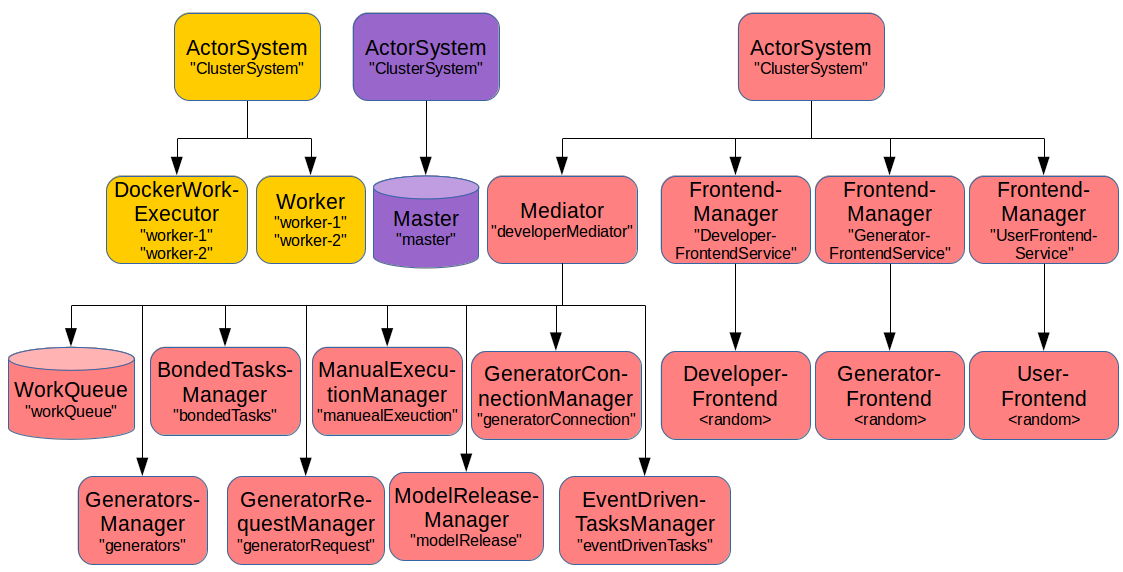
\includegraphics[width=5in]{figures/actor_hierachy_final.png}
    \caption{Zielzustand - Actor Hierachie}
    \label{fig:ZETA_HIERACHY_NEW}
\end{figure}



\chapter{Resümee}
\label{sec:SUMMARY}

\section{Schlussfolgerungen}
\label{sec:SUMMARY_CONCLUSION}

\section{Ausblick}
\label{sec:SUMMARY_OUTLOOK}



\renewcommand\thesection{A.\arabic{section}}
\renewcommand\thesubsection{\thesection.\arabic{subsection}}

\chapter*{Anhänge}
\label{chap:APPENDIX}
\addcontentsline{toc}{chapter}{Anhänge}

\pagenumbering{arabic}
\setcounter{page}{1}
\renewcommand{\thepage}{A-\arabic{page}}


\section{Abbildungen}
\label{sec:APPENDIX_FIGURES}

\section{Quelltexte}
\label{sec:APPENDIX_LISTINGS}

\renewcommand{\baselinestretch}{1}

\clearpage


\phantomsection
\renewcommand{\bibname}{Quellenverzeichnis}
\bibliography{references}
\bibliographystyle{apalike}
\newpage


\end{document}
